
%% bare_jrnl.tex
%% V1.4b
%% 2015/08/26
%% by Michael Shell
%% see http://www.michaelshell.org/
%% for current contact information.
%%
%% This is a skeleton file demonstrating the use of IEEEtran.cls
%% (requires IEEEtran.cls version 1.8b or later) with an IEEE
%% journal paper.
%%
%% Support sites:
%% http://www.michaelshell.org/tex/ieeetran/
%% http://www.ctan.org/pkg/ieeetran
%% and
%% http://www.ieee.org/

%%*************************************************************************
%% Legal Notice:
%% This code is offered as-is without any warranty either expressed or
%% implied; without even the implied warranty of MERCHANTABILITY or
%% FITNESS FOR A PARTICULAR PURPOSE! 
%% User assumes all risk.
%% In no event shall the IEEE or any contributor to this code be liable for
%% any damages or losses, including, but not limited to, incidental,
%% consequential, or any other damages, resulting from the use or misuse
%% of any information contained here.
%%
%% All comments are the opinions of their respective authors and are not
%% necessarily endorsed by the IEEE.
%%
%% This work is distributed under the LaTeX Project Public License (LPPL)
%% ( http://www.latex-project.org/ ) version 1.3, and may be freely used,
%% distributed and modified. A copy of the LPPL, version 1.3, is included
%% in the base LaTeX documentation of all distributions of LaTeX released
%% 2003/12/01 or later.
%% Retain all contribution notices and credits.
%% ** Modified files should be clearly indicated as such, including  **
%% ** renaming them and changing author support contact information. **
%%*************************************************************************


% *** Authors should verify (and, if needed, correct) their LaTeX system  ***
% *** with the testflow diagnostic prior to trusting their LaTeX platform ***
% *** with production work. The IEEE's font choices and paper sizes can   ***
% *** trigger bugs that do not appear when using other class files.       ***                          ***
% The testflow support page is at:
% http://www.michaelshell.org/tex/testflow/



\documentclass[journal]{IEEEtran}
%
% If IEEEtran.cls has not been installed into the LaTeX system files,
% manually specify the path to it like:
% \documentclass[journal]{../sty/IEEEtran}





% Some very useful LaTeX packages include:
% (uncomment the ones you want to load)


% *** MISC UTILITY PACKAGES ***
%
%\usepackage{ifpdf}
% Heiko Oberdiek's ifpdf.sty is very useful if you need conditional
% compilation based on whether the output is pdf or dvi.
% usage:
% \ifpdf
%   % pdf code
% \else
%   % dvi code
% \fi
% The latest version of ifpdf.sty can be obtained from:
% http://www.ctan.org/pkg/ifpdf
% Also, note that IEEEtran.cls V1.7 and later provides a builtin
% \ifCLASSINFOpdf conditional that works the same way.
% When switching from latex to pdflatex and vice-versa, the compiler may
% have to be run twice to clear warning/error messages.





% *** CITATION PACKAGES ***
%
\usepackage{cite}
% cite.sty was written by Donald Arseneau
% V1.6 and later of IEEEtran pre-defines the format of the cite.sty package
% \cite{} output to follow that of the IEEE. Loading the cite package will
% result in citation numbers being automatically sorted and properly
% "compressed/ranged". e.g., [1], [9], [2], [7], [5], [6] without using
% cite.sty will become [1], [2], [5]--[7], [9] using cite.sty. cite.sty's
% \cite will automatically add leading space, if needed. Use cite.sty's
% noadjust option (cite.sty V3.8 and later) if you want to turn this off
% such as if a citation ever needs to be enclosed in parenthesis.
% cite.sty is already installed on most LaTeX systems. Be sure and use
% version 5.0 (2009-03-20) and later if using hyperref.sty.
% The latest version can be obtained at:
% http://www.ctan.org/pkg/cite
% The documentation is contained in the cite.sty file itself.



% \usepackage{graphicx}
% \usepackage{subfigure}
% \usepackage{threeparttable}
% \usepackage{enumitem}
% \usepackage{bigstrut,multirow}
% \usepackage{algorithm}  
% \usepackage{algorithmicx}  
% \usepackage{algpseudocode}  
% \usepackage{amsmath} 
% \usepackage{lipsum}
% \usepackage{cleveref}



% *** GRAPHICS RELATED PACKAGES ***
%
% \ifCLASSINFOpdf
\usepackage[pdftex]{graphicx}
  % declare the path(s) where your graphic files are
  % \graphicspath{{../pdf/}{../jpeg/}}
  % and their extensions so you won't have to specify these with
  % every instance of \includegraphics
  % \DeclareGraphicsExtensions{.pdf,.jpeg,.png}
% \else
  % or other class option (dvipsone, dvipdf, if not using dvips). graphicx
  % will default to the driver specified in the system graphics.cfg if no
  % driver is specified.
  % \usepackage[dvips]{graphicx}
  % declare the path(s) where your graphic files are
  % \graphicspath{{../eps/}}
  % and their extensions so you won't have to specify these with
  % every instance of \includegraphics
  % \DeclareGraphicsExtensions{.eps}
% \fi
% graphicx was written by David Carlisle and Sebastian Rahtz. It is
% required if you want graphics, photos, etc. graphicx.sty is already
% installed on most LaTeX systems. The latest version and documentation
% can be obtained at: 
% http://www.ctan.org/pkg/graphicx
% Another good source of documentation is "Using Imported Graphics in
% LaTeX2e" by Keith Reckdahl which can be found at:
% http://www.ctan.org/pkg/epslatex
%
% latex, and pdflatex in dvi mode, support graphics in encapsulated
% postscript (.eps) format. pdflatex in pdf mode supports graphics
% in .pdf, .jpeg, .png and .mps (metapost) formats. Users should ensure
% that all non-photo figures use a vector format (.eps, .pdf, .mps) and
% not a bitmapped formats (.jpeg, .png). The IEEE frowns on bitmapped formats
% which can result in "jaggedy"/blurry rendering of lines and letters as
% well as large increases in file sizes.
%
% You can find documentation about the pdfTeX application at:
% http://www.tug.org/applications/pdftex





% *** MATH PACKAGES ***
%
\usepackage{amsmath}
% A popular package from the American Mathematical Society that provides
% many useful and powerful commands for dealing with mathematics.
%
% Note that the amsmath package sets \interdisplaylinepenalty to 10000
% thus preventing page breaks from occurring within multiline equations. Use:
%\interdisplaylinepenalty=2500
% after loading amsmath to restore such page breaks as IEEEtran.cls normally
% does. amsmath.sty is already installed on most LaTeX systems. The latest
% version and documentation can be obtained at:
% http://www.ctan.org/pkg/amsmath





% *** SPECIALIZED LIST PACKAGES ***
%
\usepackage{algorithmic}
% algorithmic.sty was written by Peter Williams and Rogerio Brito.
% This package provides an algorithmic environment fo describing algorithms.
% You can use the algorithmic environment in-text or within a figure
% environment to provide for a floating algorithm. Do NOT use the algorithm
% floating environment provided by algorithm.sty (by the same authors) or
% algorithm2e.sty (by Christophe Fiorio) as the IEEE does not use dedicated
% algorithm float types and packages that provide these will not provide
% correct IEEE style captions. The latest version and documentation of
% algorithmic.sty can be obtained at:
% http://www.ctan.org/pkg/algorithms
% Also of interest may be the (relatively newer and more customizable)
% algorithmicx.sty package by Szasz Janos:
% http://www.ctan.org/pkg/algorithmicx




% *** ALIGNMENT PACKAGES ***
%
\usepackage{array}
% Frank Mittelbach's and David Carlisle's array.sty patches and improves
% the standard LaTeX2e array and tabular environments to provide better
% appearance and additional user controls. As the default LaTeX2e table
% generation code is lacking to the point of almost being broken with
% respect to the quality of the end results, all users are strongly
% advised to use an enhanced (at the very least that provided by array.sty)
% set of table tools. array.sty is already installed on most systems. The
% latest version and documentation can be obtained at:
% http://www.ctan.org/pkg/array


% IEEEtran contains the IEEEeqnarray family of commands that can be used to
% generate multiline equations as well as matrices, tables, etc., of high
% quality.




% *** SUBFIGURE PACKAGES ***
%\ifCLASSOPTIONcompsoc
% \usepackage[caption=false,font=normalsize,labelfont=sf,textfont=sf]{subfig}
%\else
\usepackage[caption=false,font=footnotesize]{subfig}
%\fi
% subfig.sty, written by Steven Douglas Cochran, is the modern replacement
% for subfigure.sty, the latter of which is no longer maintained and is
% incompatible with some LaTeX packages including fixltx2e. However,
% subfig.sty requires and automatically loads Axel Sommerfeldt's caption.sty
% which will override IEEEtran.cls' handling of captions and this will result
% in non-IEEE style figure/table captions. To prevent this problem, be sure
% and invoke subfig.sty's "caption=false" package option (available since
% subfig.sty version 1.3, 2005/06/28) as this is will preserve IEEEtran.cls
% handling of captions.
% Note that the Computer Society format requires a larger sans serif font
% than the serif footnote size font used in traditional IEEE formatting
% and thus the need to invoke different subfig.sty package options depending
% on whether compsoc mode has been enabled.
%
% The latest version and documentation of subfig.sty can be obtained at:
% http://www.ctan.org/pkg/subfig




% *** FLOAT PACKAGES ***
%
\usepackage{fixltx2e}
% fixltx2e, the successor to the earlier fix2col.sty, was written by
% Frank Mittelbach and David Carlisle. This package corrects a few problems
% in the LaTeX2e kernel, the most notable of which is that in current
% LaTeX2e releases, the ordering of single and double column floats is not
% guaranteed to be preserved. Thus, an unpatched LaTeX2e can allow a
% single column figure to be placed prior to an earlier double column
% figure.
% Be aware that LaTeX2e kernels dated 2015 and later have fixltx2e.sty's
% corrections already built into the system in which case a warning will
% be issued if an attempt is made to load fixltx2e.sty as it is no longer
% needed.
% The latest version and documentation can be found at:
% http://www.ctan.org/pkg/fixltx2e


\usepackage{stfloats}
% stfloats.sty was written by Sigitas Tolusis. This package gives LaTeX2e
% the ability to do double column floats at the bottom of the page as well
% as the top. (e.g., "\begin{figure*}[!b]" is not normally possible in
% LaTeX2e). It also provides a command:
%\fnbelowfloat
% to enable the placement of footnotes below bottom floats (the standard
% LaTeX2e kernel puts them above bottom floats). This is an invasive package
% which rewrites many portions of the LaTeX2e float routines. It may not work
% with other packages that modify the LaTeX2e float routines. The latest
% version and documentation can be obtained at:
% http://www.ctan.org/pkg/stfloats
% Do not use the stfloats baselinefloat ability as the IEEE does not allow
% \baselineskip to stretch. Authors submitting work to the IEEE should note
% that the IEEE rarely uses double column equations and that authors should try
% to avoid such use. Do not be tempted to use the cuted.sty or midfloat.sty
% packages (also by Sigitas Tolusis) as the IEEE does not format its papers in
% such ways.
% Do not attempt to use stfloats with fixltx2e as they are incompatible.
% Instead, use Morten Hogholm'a dblfloatfix which combines the features
% of both fixltx2e and stfloats:
%
% \usepackage{dblfloatfix}
% The latest version can be found at:
% http://www.ctan.org/pkg/dblfloatfix

\usepackage{cleveref}
\crefname{figure}{fig.}{fig.}

%\ifCLASSOPTIONcaptionsoff
%  \usepackage[nomarkers]{endfloat}
% \let\MYoriglatexcaption\caption
% \renewcommand{\caption}[2][\relax]{\MYoriglatexcaption[#2]{#2}}
%\fi
% endfloat.sty was written by James Darrell McCauley, Jeff Goldberg and 
% Axel Sommerfeldt. This package may be useful when used in conjunction with 
% IEEEtran.cls'  captionsoff option. Some IEEE journals/societies require that
% submissions have lists of figures/tables at the end of the paper and that
% figures/tables without any captions are placed on a page by themselves at
% the end of the document. If needed, the draftcls IEEEtran class option or
% \CLASSINPUTbaselinestretch interface can be used to increase the line
% spacing as well. Be sure and use the nomarkers option of endfloat to
% prevent endfloat from "marking" where the figures would have been placed
% in the text. The two hack lines of code above are a slight modification of
% that suggested by in the endfloat docs (section 8.4.1) to ensure that
% the full captions always appear in the list of figures/tables - even if
% the user used the short optional argument of \caption[]{}.
% IEEE papers do not typically make use of \caption[]'s optional argument,
% so this should not be an issue. A similar trick can be used to disable
% captions of packages such as subfig.sty that lack options to turn off
% the subcaptions:
% For subfig.sty:
% \let\MYorigsubfloat\subfloat
% \renewcommand{\subfloat}[2][\relax]{\MYorigsubfloat[]{#2}}
% However, the above trick will not work if both optional arguments of
% the \subfloat command are used. Furthermore, there needs to be a
% description of each subfigure *somewhere* and endfloat does not add
% subfigure captions to its list of figures. Thus, the best approach is to
% avoid the use of subfigure captions (many IEEE journals avoid them anyway)
% and instead reference/explain all the subfigures within the main caption.
% The latest version of endfloat.sty and its documentation can obtained at:
% http://www.ctan.org/pkg/endfloat
%
% The IEEEtran \ifCLASSOPTIONcaptionsoff conditional can also be used
% later in the document, say, to conditionally put the References on a 
% page by themselves.




% *** PDF, URL AND HYPERLINK PACKAGES ***
%
\usepackage{url}
% url.sty was written by Donald Arseneau. It provides better support for
% handling and breaking URLs. url.sty is already installed on most LaTeX
% systems. The latest version and documentation can be obtained at:
% http://www.ctan.org/pkg/url
% Basically, \url{my_url_here}.


\usepackage{color}
\usepackage{multirow}
\usepackage{amsfonts}
\usepackage{threeparttable}
\usepackage{bigstrut}
% *** Do not adjust lengths that control margins, column widths, etc. ***
% *** Do not use packages that alter fonts (such as pslatex).         ***
% There should be no need to do such things with IEEEtran.cls V1.6 and later.
% (Unless specifically asked to do so by the journal or conference you plan
% to submit to, of course. )


% correct bad hyphenation here
\hyphenation{op-tical net-works semi-conduc-tor}


\begin{document}
%
% paper title
% Titles are generally capitalized except for words such as a, an, and, as,
% at, but, by, for, in, nor, of, on, or, the, to and up, which are usually
% not capitalized unless they are the first or last word of the title.
% Linebreaks \\ can be used within to get better formatting as desired.
% Do not put math or special symbols in the title.
\title{INCAME : Interruptible CNN Accelerator for Multi-robot Exploration}
%
%
% author names and IEEE memberships
% note positions of commas and nonbreaking spaces ( ~ ) LaTeX will not break
% a structure at a ~ so this keeps an author's name from being broken across
% two lines.
% use \thanks{} to gain access to the first footnote area
% a separate \thanks must be used for each paragraph as LaTeX2e's \thanks
% was not built to handle multiple paragraphs
%

% \author{Michael~Shell,~\IEEEmembership{Member,~IEEE,}
%         John~Doe,~\IEEEmembership{Fellow,~OSA,}
%         and~Jane~Doe,~\IEEEmembership{Life~Fellow,~IEEE}% <-this % stops a space
% \thanks{M. Shell was with the Department
% of Electrical and Computer Engineering, Georgia Institute of Technology, Atlanta,
% GA, 30332 USA e-mail: (see http://www.michaelshell.org/contact.html).}% <-this % stops a space
% \thanks{J. Doe and J. Doe are with Anonymous University.}% <-this % stops a space
% \thanks{Manuscript received April 19, 2005; revised August 26, 2015.}}


\author{Jincheng Yu,
        Zhilin Xu,
        Shulin Zeng,
        Chao Yu,
        Jiantao Qiu,
        Chaoyang Shen,
        Yuanfan Xu, \\
        Guohao Dai,
        Yu Wang,
        and Huazhong Yang % <-this % stops a space
\thanks{This work is supported by National Key Research and Development Program of China (No. 2017YFA0207600 ), National Natural Science Foundation of China (No. U19B2019, 61832007 ), Tsinghua EE Xilinx AI Research Fund, Beijing National Research Center for Information Science and Technology (BNRist), and Beijing Innovation Center for Future Chips.
}% <-this % stops a space
\thanks{All authors are from Department of Electronic Engineering, Tsinghua University, Beijing, China.}% <-this % stops a space
\thanks{Email: yjc16@mails.tsinghua.edu.cn; yu-wang@mail.tsinghua.edu.cn} }

% note the % following the last \IEEEmembership and also \thanks - 
% these prevent an unwanted space from occurring between the last author name
% and the end of the author line. i.e., if you had this:
% 
% \author{....lastname \thanks{...} \thanks{...} }
%                     ^------------^------------^----Do not want these spaces!
%
% a space would be appended to the last name and could cause every name on that
% line to be shifted left slightly. This is one of those "LaTeX things". For
% instance, "\textbf{A} \textbf{B}" will typeset as "A B" not "AB". To get
% "AB" then you have to do: "\textbf{A}\textbf{B}"
% \thanks is no different in this regard, so shield the last } of each \thanks
% that ends a line with a % and do not let a space in before the next \thanks.
% Spaces after \IEEEmembership other than the last one are OK (and needed) as
% you are supposed to have spaces between the names. For what it is worth,
% this is a minor point as most people would not even notice if the said evil
% space somehow managed to creep in.



% The paper headers
% \markboth{Journal of \LaTeX\ Class Files,~Vol.~14, No.~8, August~2015}%
% {Shell \MakeLowercase{\textit{et al.}}: Bare Demo of IEEEtran.cls for IEEE Journals}
% The only time the second header will appear is for the odd numbered pages
% after the title page when using the twoside option.
% 
% *** Note that you probably will NOT want to include the author's ***
% *** name in the headers of peer review papers.                   ***
% You can use \ifCLASSOPTIONpeerreview for conditional compilation here if
% you desire.




% If you want to put a publisher's ID mark on the page you can do it like
% this:
%\IEEEpubid{0000--0000/00\$00.00~\copyright~2015 IEEE}
% Remember, if you use this you must call \IEEEpubidadjcol in the second
% column for its text to clear the IEEEpubid mark.



% use for special paper notices
%\IEEEspecialpapernotice{(Invited Paper)}


% make the title area
\maketitle

% As a general rule, do not put math, special symbols or citations
% in the abstract or keywords.
\begin{abstract}
% Multi-Robot Exploration (MR-Exploration) that provides the location and map is the basic task for many multi-robot applications. 
% With the development of Convolutional Neural Network (CNN), the accuracy of some critical components in MR-Exploration, such as Feature-point Extraction (FE) and Place Recognition (PR), can significantly benefit from CNN. 
% To deploy CNN on the embedded real-time system, previous works design CNN accelerators on FPGA. 
% However, these accelerators mainly focus on improving the performance of a single network, lacking support for multi-task. 
% Since researchers in robotic usually run different CNN tasks simultaneously, the inability of accelerators to support multi-task makes it difficult for researchers in robotic to use embedded FPGA. 
% Furthermore, the post-processing of  CNN-based components (such as FE and PR), which is also computation consuming, becomes the bottleneck of the system, after accelerating the CNN backbones.

Multi-Robot Exploration (MR-Exploration) that provides the location and map is a primary task for many multi-robot applications. Recent researches introduce Convolutional Neural Network (CNN) into critical components in MR-Exploration, such as Feature-point Extraction (FE) and Place Recognition (PR), to improve the system performance. This CNN-based MR-Exploration needs to run multiple CNN models and complex post-processing algorithms simultaneously, which significantly challenges the hardware platforms of embedded systems.
Previous researches have shown that FPGA is ideal for CNN processing on embedded platforms. However, such accelerators usually process different models in sequence and cannot schedule multiple tasks at runtime. Furthermore, the post-processing of CNNs is also computationally intensive and becomes the bottleneck of the whole system.

To handle such problems, we propose an INterruptible CNN Accelerator for Multi-Robot Exploration (INCAME) framework for the rapid deployment of robot applications on FPGA. In INCAME, we propose an interrupt method based on virtual instructions to support multi-task on CNN accelerators. INCAME also includes hardware modules to accelerate the post-processing of the CNN-based components, organically integrates the post-processing and CNN backbone by sharing memory.
Experimental results show that INCAME enables multi-task scheduling on the CNN accelerator with negligible performance degradation (0.3\%). With the help of multi-task supporting and post-processing acceleration, INCAME enables embedded FPGA to perform MR-Exploration in real time (20 fps).

% To handle such problems, we propose an INterruptible CNN Accelerator for Multi-Robot Exploration (INCAME) framework for rapid deployment of MR-Exploration on FPGA.
% In INCAME, we propose a virtual-instruction-based interrupt method to support multi-task on CNN accelerators.
% INCAME also includes hardware modules to accelerate the post-processing of the CNN-based components.
% % We evaluate INCAME on Xilinx ZU9 MPSoC. 
% The experiment results show that INCAME enables multi-task scheduling on the CNN accelerator with negligible performance reduction (0.8\%). With the help of multi-task supporting and post-processing accelerating, INCAME enables embedded FPGA to execute MR-Exploration in real time (20 fps).
% Multi-Robot Exploration (MR-Exploration) that provides the location and maps is the basic task for many multi-robot applications. 
% Feature-point Extraction (FE) and Place Recognition (PR) are two critical modules in MR-Exploration.
% The accuracy of both modules can benefit from Convolutional Neural Network (CNN).
% Previous CNN accelerators on FPGA mainly focus on improving the performance of a single neural network, lacking multi-task support.
% Researchers in robotic usually run several CNN tasks simultaneously, such as FE and PR.
% The inability of CNN accelerators to support multi-task makes it difficult for researchers in robotic to use embedded FPGA.

% We propose a \textit{MU}lti-\textit{RO}bot \textit{EX}ploration \textit{E}ngine (MUROEXE) to deploy MR-Exploration on embedded FPGA. 
% We propose a virtual-instruction-based interrupt method to support multi-task on CNN accelerators.
% Besides the CNN backbone, the post-precessing for CNN-based FE and PR is also computation consuming. 
% MUROEXE introduces RTL/HLS modules to accelerate the post-precessing of CNN-based modules.
% Experiments show that MUROEXE supports multi-thread scheduling with negligible performance reduction (??\%).
% MUROEXE enables embedded FPGA (Xilinx ZU9) executing MR-Exploration in real-time (30 fps).
\end{abstract}

% Note that keywords are not normally used for peerreview papers.
% \begin{IEEEkeywords}
% IEEE, IEEEtran, journal, \LaTeX, paper, template.
% \end{IEEEkeywords}






% For peer review papers, you can put extra information on the cover
% page as needed:
% \ifCLASSOPTIONpeerreview
% \begin{center} \bfseries EDICS Category: 3-BBND \end{center}
% \fi
%
% For peerreview papers, this IEEEtran command inserts a page break and
% creates the second title. It will be ignored for other modes.
\IEEEpeerreviewmaketitle


\section{INTRODUCTION}
\label{sec:intro}

The cooperation of agents can expand the capability of the unmanned system, and the multi-agent intelligent system is a promising research field.
Multi-Robot Exploration (MR-Exploration)  ~\cite{corah2019communication} provides location and map for each robot, and is the basic task for many multi-robot applications, such as multi-robot navigation  ~\cite{tanner2005towards} and multi-robot rescue  ~\cite{baxter2007multi}.


\begin{figure}[t]
    \centering
    % \vspace{-0.1cm} 
    % \setlength{\abovecaptionskip}{0cm} 
    % \setlength{\belowcaptionskip}{-0.4cm} 
	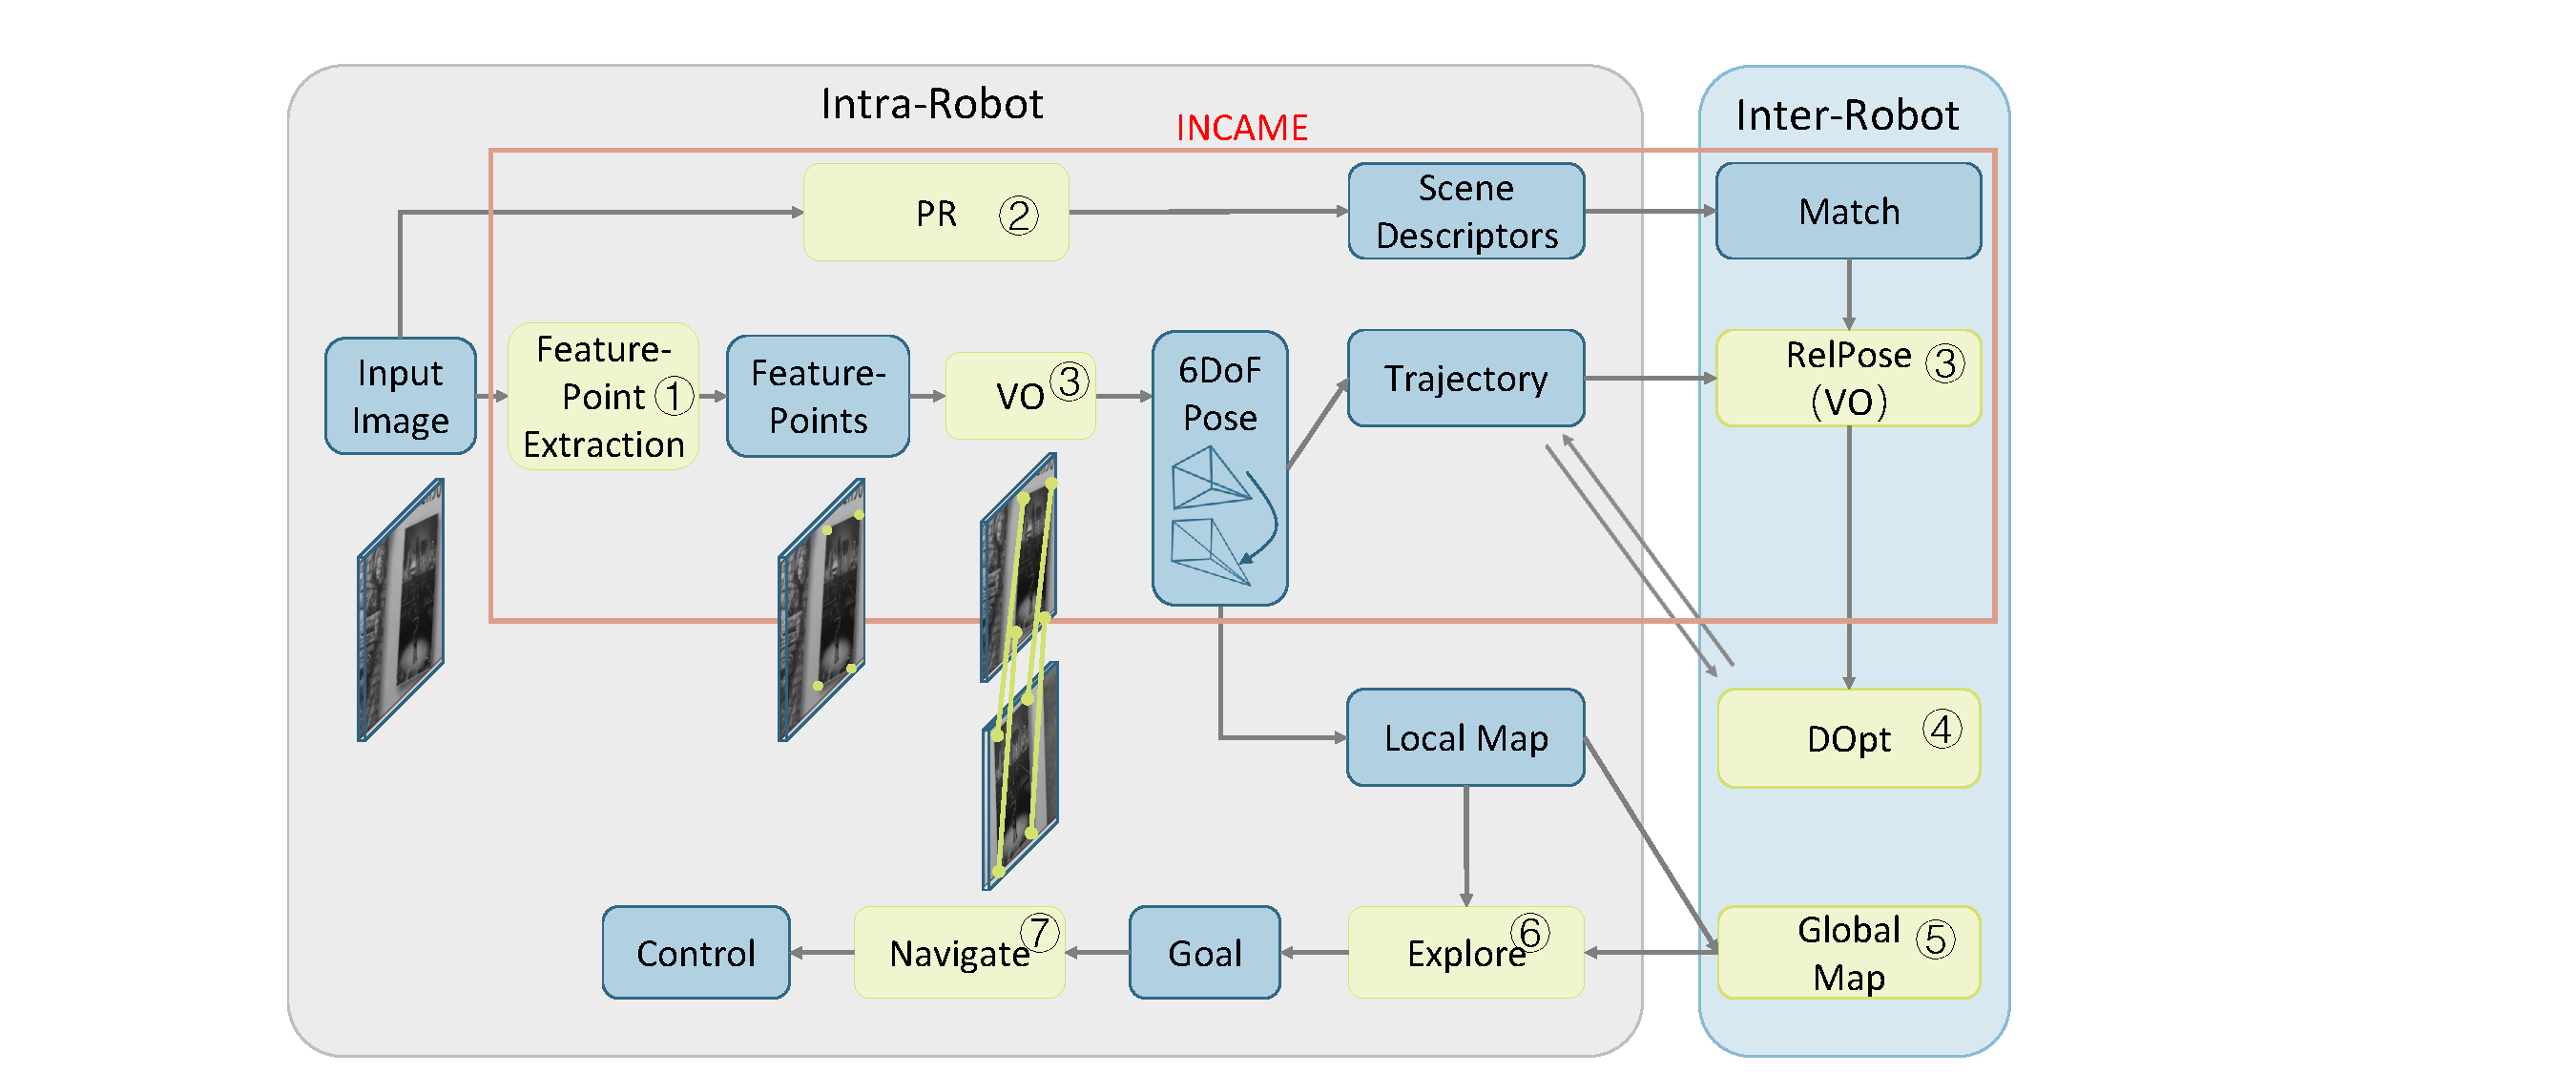
\includegraphics[width=0.99\linewidth]{fig/maexp.pdf}
     \caption{
        The components in MR-Exploration.  Each frame is required to execute \textcircled{1}\textcircled{3} with low latency. \textcircled{2} runs on some keyframes. INCAME implements \textcircled{1} \textcircled{2} on the CNN accelerator, and optimizes the scheduling among \textcircled{1} \textcircled{2} \textcircled{3}.
    }
%     \caption{
%         The components in MR-Exploration. \textcircled{1}\textcircled{3} are basic for a single robot, should be execute every frame. \textcircled{2} generates representation code for some keyframes. \textcircled{4}\textcircled{5} are only executed when representation codes are matched across robots and they are latency tolerant.  \textcircled{6}\textcircled{7} are used for decision and navigation, also latency tolerant.
%     }
	\label{fig:maexp}
\end{figure}

The  MR-Exploration system  ~\cite{corah2019communication, cieslewski2018data} consists of several robots, and each robot executes the system illustrated in \Cref{fig:maexp}. Each input frame is fed to the Feature-point Extraction (FE, \textcircled{1}) module for Visual Odometry (VO). 
Some input frames, called keyframes, are fed to the Place Recognition (PR, \textcircled{2}) module.
PR module generates the compact image representation, which produces the candidate place recognition matches between different robots. 
The Visual Odometry (VO) (\textcircled{3}) matches the feature-points of two adjacent frames to produce the 6 Degrees of Freedom (6-DoF) poses. 
\textcolor{blue}{
Although the VO outputs the 6-DoF poses, which is represents the pose in 3D space, we build the 2D map only using several lines of the camera. 
By projecting the 3D poses into 2D map to navigate the robots, we significantly reduce the computational cost of building maps.
Furthermore, each 2D map is aligned to a key-frame \cite{ho2018virtual,sodhi2019online}.
Through optimizing the keyframe trajectory poses, the map can be synchronously optimized and merged.
}
% Based on the 6-DoF poses,  map and the trajectory can be used for location.
The relative pose (RelPose) module does the same operation as VO(\textcircled{3}) and establishes relative poses between the candidate place matches of different robots. 
The decentralized optimization module (DOpt, \textcircled{4}) optimizes the intra-robot relative pose measurements from VO and the inter-robot relative pose measurements from RelPose. 
\textcolor{blue}{
We use the Pose Graph Optimization (PGO) \cite{Choudhary:2017e66} to do DOpt. 
PGO only optimizes the keyframe trajectory pose without optimizing the keypoints. 
Because the number of keyframe is far less than the number of feature-points, PGO is much faster than Bundle Adjustment (BA) algorithm \cite{wu2011multicore}, which not only optimize the trajectory but also the feature-points.
}
The global map generation module (\textcircled{5}) merges the maps. The exploration module (\textcircled{6}) decides an unexplored goal point for each robot to move based on the merged map and the estimated location. The navigation module (\textcircled{7}) guides each robot to the goal point, including path planning and obstacle avoidance.

\textcolor{blue}{
With the help of 2D maps (\textcircled{5}) and fast PGO (\textcircled{4}), we deploy map merging and optimization on the embedded CPU. 
PR (\textcircled{2}), feature-point extraction (\textcircled{1}), and VO (\textcircled{3}) become the most computational intensive modules. We optimize the scheduling these components across the CPU side (processing system, PS) and FPGA side (programmable logic, PL), on Xilinx MPSoC  ~\cite{MPSoC}.
}



% \Cref{fig:maexp} illustrates the computation modules in MR-Exploration.
% Feature-point extraction (\textcircled{1}) and visual odometry (VO, \textcircled{3}) should be performed for each input frame, and should be completed before the next frame. 
% Place Recognition (PR, \textcircled{2}) generates the representation code for some keyframes, and sends them to other robots. 
% When the  representation codes from different robots are matched, optimization (\textcircled{7}) and map merging ((\textcircled{8})) are performed to merge the trajectories and maps. \textcircled{4}\textcircled{5}\textcircled{6} are for decision-making and navigation based on the merged maps. 




\begin{figure*}[t]
    % \flushleft
    \centering
    % \vspace{-0.3cm} 
    % \setlength{\abovecaptionskip}{0cm} 
    % \setlength{\belowcaptionskip}{-0.2cm} 
    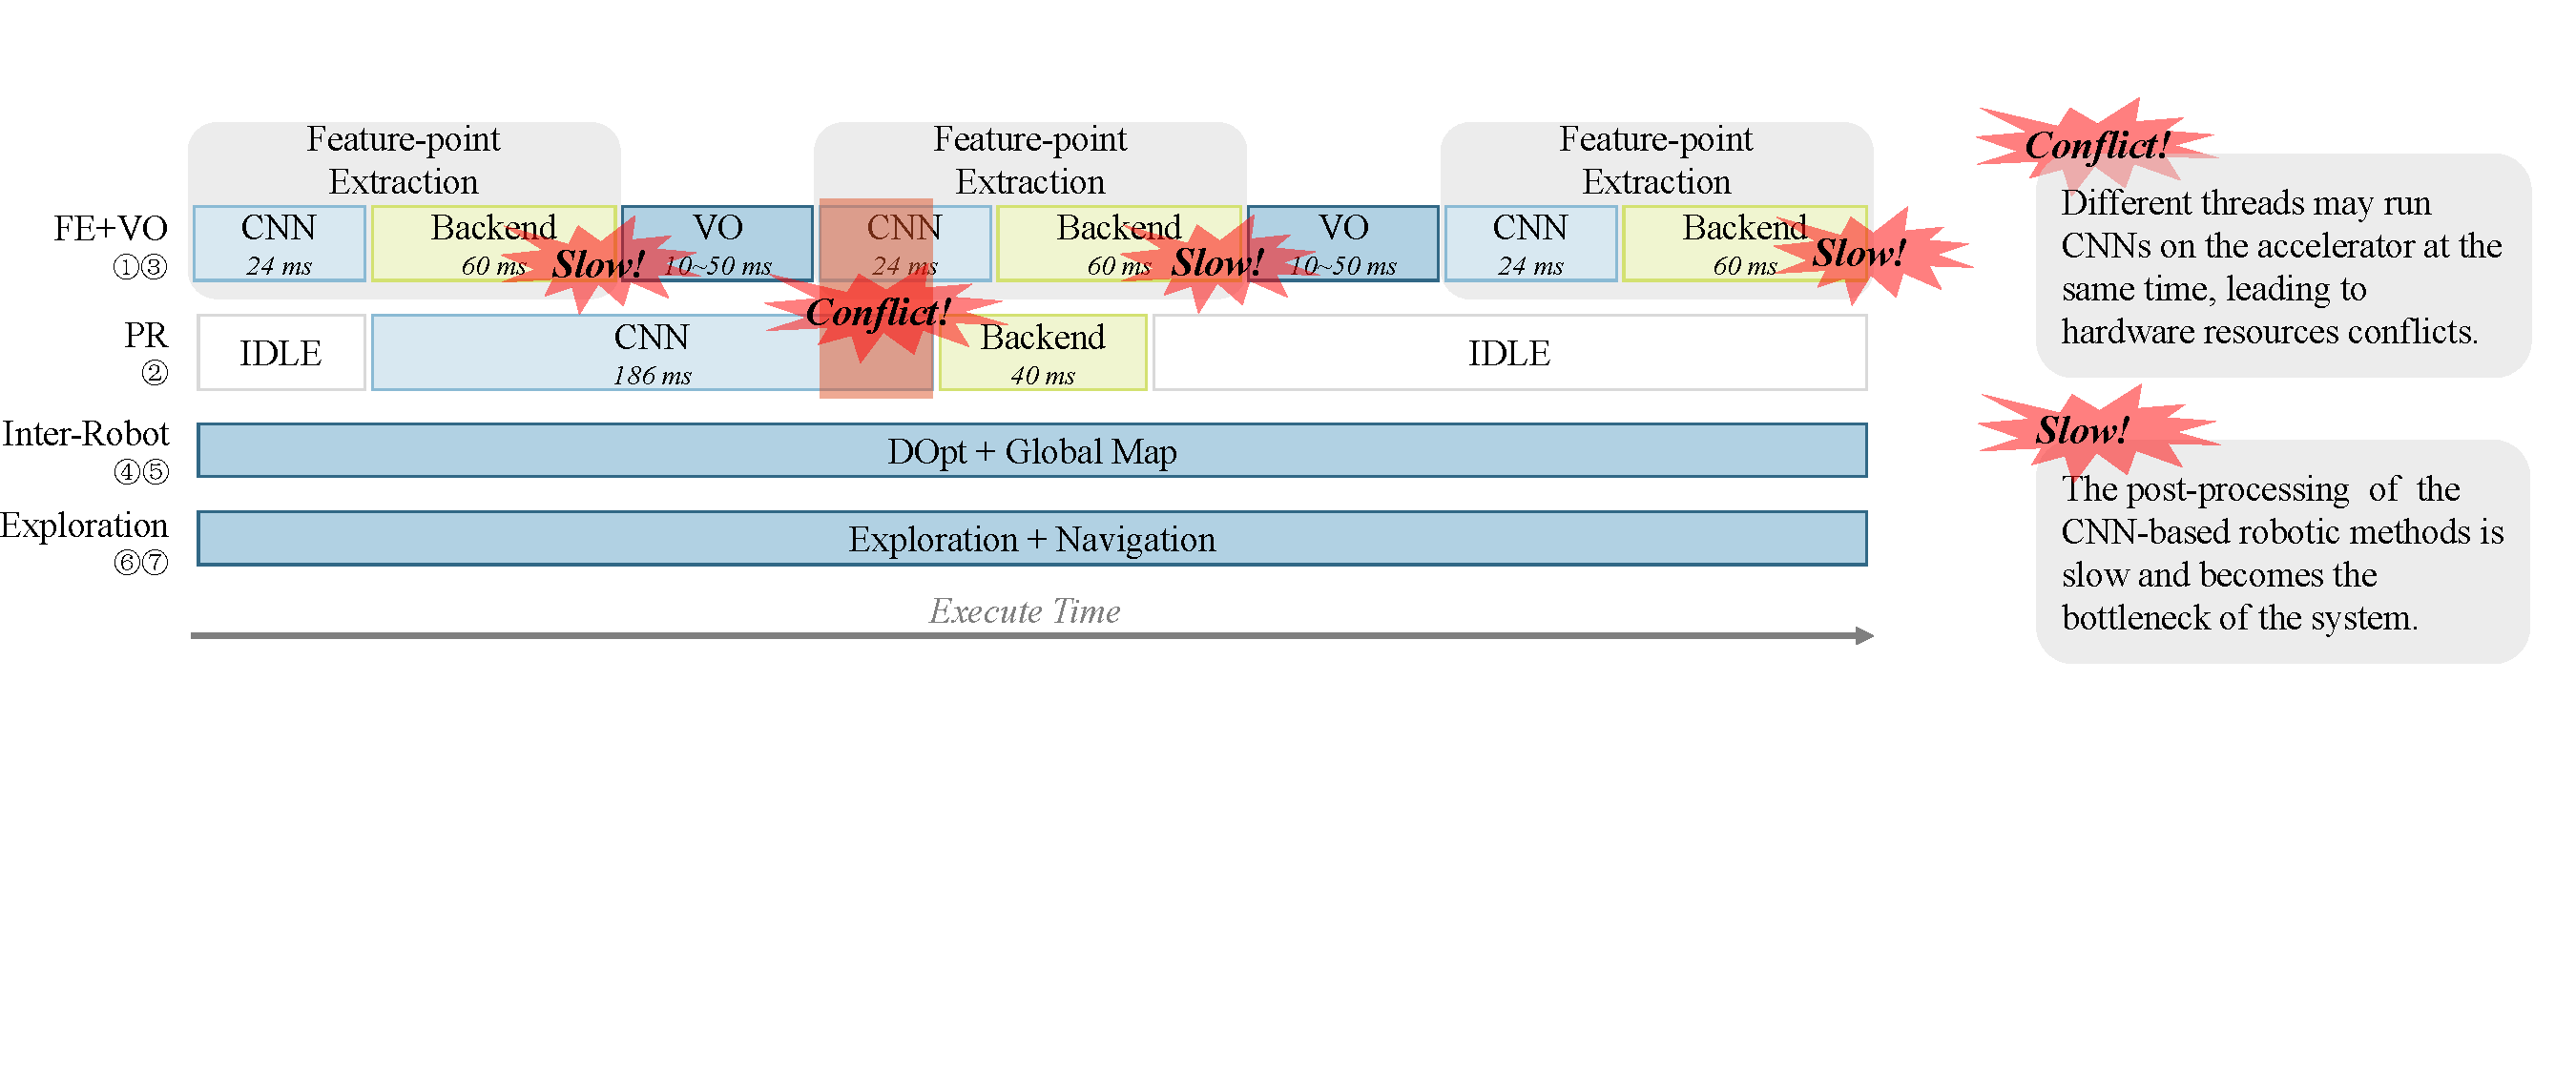
\includegraphics[width=0.99\textwidth]{fig/overalltime.pdf} 	
    \vspace{-2mm}
    \caption{
    The overall timeline of MR-Exploration. The FPGA accelerator is adapted in the feature-point extraction (FE) and place recognition (PR). The simultaneous occupancy of a single FPGA accelerator by these two software threads will lead to hardware resources conflicts. The post-processing of the visual odometry (VO) with feature-points on embedded CPU is time-costing and cannot meet the real-time requirements.
    }
	\label{fig:overalltime}
\end{figure*}

Recent works use CNN to extract feature-points  ~\cite{detone2018superpoint, simo2015discriminative, yi2016lift} and generate the place representation code  ~\cite{arandjelovic2016netvlad, radenovic2018fine}. 
Compared with the popular handcrafted extraction method, ORB ~\cite{Mur-Artal:2017281}, the CNN-based feature-point extraction method, SuperPoint  ~\cite{detone2018superpoint}, achieves 10\%-30\% higher matching accuracy.
The accuracy of the place recognition code based on another CNN-based method, GeM  ~\cite{radenovic2018fine}, is also about 20\% better than the handcrafted method, rootSIFT  ~\cite{jegou2014triang}.

% Thus, we adopt these CNN methods to realize Feature-point Extraction and  Place Recognition. 
Therefore, CNN is increasingly used in robotic systems. 
Besides these two components, more CNN-based methods, such as semantic segmentation  ~\cite{long2015fully} and object detection  ~\cite{ren2015faster}, can be introduced into robots to achieve better performance in the future. 

However, CNN is computation consuming. A single inference of the CNN-based SuperPoint feature-point extraction consumes 39G operations  ~\cite{detone2018superpoint}, while a single inference of the CNN-based GeM  place recognition consumes 192G operations  ~\cite{radenovic2018fine}.
Therefore, specific hardware architectures on FPGA  ~\cite{guo2017angel,yu2018instruction,li_high_2016,qiu2016going,lu_evaluating_2017} are designed to deploy CNN on the embedded system.
With the help of neural network quantization and on-chip data reuse, the speed of CNN accelerators on embedded FPGA achieves 3TOP/s  ~\cite{lu_evaluating_2017}, which can support the real-time execution of CNN-based feature-point extraction  ~\cite{detone2018superpoint}.
However, these CNN accelerators are designed and optimized to accelerate a single CNN. They cannot automatically schedule two or more tasks simultaneously. 
% Even if only FE and PR are implemented in CNN, the computational complexity reaches 1 TOP/s , which poses a challenge to the real-time performance of embedded systems.


% In recent years, FPGA is becoming a promising platform for algorithm acceleration. 

We do a simple profiling of MR-Exploration with the CNN accelerator. The CNN backbones of FE and  PR are executed on the FPGA accelerator (Angel-Eye ~\cite{guo2017angel}).
Other operations, including the post-processing of the CNN-based FE and PR, run on the PS side of Xilinx ZCU102 evaluation board ~\cite{zcu102}. The timeline of each component is illustrated in \Cref{fig:overalltime}. 
The threads of FE and PR may need to process CNN at the same time,  and the simultaneous requests of the accelerator will lead to hardware resources conflicts. For CNN accelerators, the inability of multi-task makes it difficult for researchers in robotics to use embedded FPGA.

In order to facilitate robotic researchers to run different CNN tasks simultaneously on the FPGA accelerator, the accelerator should support the following features:

\textbf{Multi-thread:} Different components in a robot are from different developers. Thus, the Robot Operating System (ROS)  ~\cite{quigley2009ros} is proposed as a middleware to fuse these independent components, and is widely used by robotic researchers. Each component is considered as an independent thread in ROS. Different threads should have independent access to the accelerator without knowing the status of others.


% A robot contains many components including perception, decision-making, and control. 
% The Robot Operating System (ROS)  ~\cite{quigley2009ros} is a popular middleware fusing different components from different developers. 
% In ROS, each module is considered as an independent thread on CPU. 
% Different threads should have easy access to the FPGA accelerator.

\textbf{Dynamic Scheduling:} The execution of CNN depends on other operations. For example, CNN-based FE (\textcircled{1} in \Cref{fig:maexp}) needs to be executed after the VO (\textcircled{3}) is completed. 
The VO is running on the CPU, and the execution time varies with the input data  ~\cite{mohanan2018survey} (10ms - 50ms in \Cref{fig:overalltime}). 
The accelerator cannot predict when to start a task. 
Therefore, the FPGA accelerator should be scheduled dynamically to support irregular task requests from the software.

\textbf{Scheduling by priority:} Different components have different priorities. The control and perception tasks usually have higher priorities, while the long-term decision and optimization have lower priorities  ~\cite{RamsauerKLM17}. The critical tasks, which are latency-sensitive,  need to be processed firstly on the accelerator.

The concept of interrupt  ~\cite{jen1974processor} is introduced to CPU in the 1960s. It enables the CPU to support dynamic multi-task scheduling according to priority to satisfy these three functions. Therefore, we introduce the concept of interrupt to the CNN accelerator in this paper to support multi-task on FPGA-based accelerators.

Besides the CNN backbones, the post-processing of the CNN-based methods, including normalization, softmax, rank, etc., are also computationally intensive. As illustrated in \Cref{fig:overalltime}, the execution time of post-processing for FE on embedded CPU (\textasciitilde 60ms) exceeds that of CNN backbone on the accelerator (\textasciitilde  30ms), and becomes the bottleneck of the system. 
As mentioned before, CNN is widely used in a variety of robot tasks.
The post-processing of these different tasks may become the new bottleneck of the system.
It is necessary to use FPGA to speed up post-processing, and a framework is also needed to organically integrate the CNN backbones and post-processing operations.

To address the above challenges, we propose an INterruptible CNN Accelerator for Multi-robot Exploration (INCAME) for rapid deployment of robot application on FPGA, with the following contributions:

\begin{itemize}
    % \begin{itemize}[leftmargin = 10 pt]
% \item We propose a CNN-based MR-Exploration framework based on FPGA. The hardware and software modules in INCAME is designed for ROS  ~\cite{quigley2009ros}, so that the modules can be easily used in other applications.
\item We propose a CNN-based MR-Exploration framework, INCAME. CNN-based methods for feature-point extraction (FE) and place recognition (PR) are accelerated with FPGA on the ROS platform ~\cite{quigley2009ros}. With the help of the unified interface in ROS, these CNN-based methods can be easily used by other developers in different applications.
\item We propose a \textbf{virtual-instruction-based} interrupt method to make the CNN accelerator support dynamic multi-task scheduling by priority. The method solves the hardware resources conflicts when accelerating different CNN tasks on ROS.
% \item We only needs to modify the instruction fetch module of the CNN accelerator in hardware to support interrupt. Thus, it is easy to be extended to different instruction-driven CNN accelerators.
\item We optimize the data flow of the post-processing operations. Hardware modules are also designed for the optimized post-processing. This software-hardware co-optimization assures the real-time performance of MR-Exploration .
\end{itemize}

The rest of this article is organized as follows: \Cref{sec:relate} introduces the related work. \Cref{sec:incame} introduces the INCAME framework with ROS. \Cref{sec:cnninterrupt} details the {virtual-instruction-based} interrupt. \Cref{sec:hardsoftcodesign} details the optimization of post-processing.  Experimental results and analysis are given in \Cref{sec:experiments}. \Cref{sec:conclusion} concludes this paper.

\section{RELATED WORK}

\label{sec:relate}


\begin{figure*}[t]
	\centering
    % \vspace{-0.1cm} 
    % \setlength{\abovecaptionskip}{0cm} 
    % \setlength{\belowcaptionskip}{-0.2cm} 
    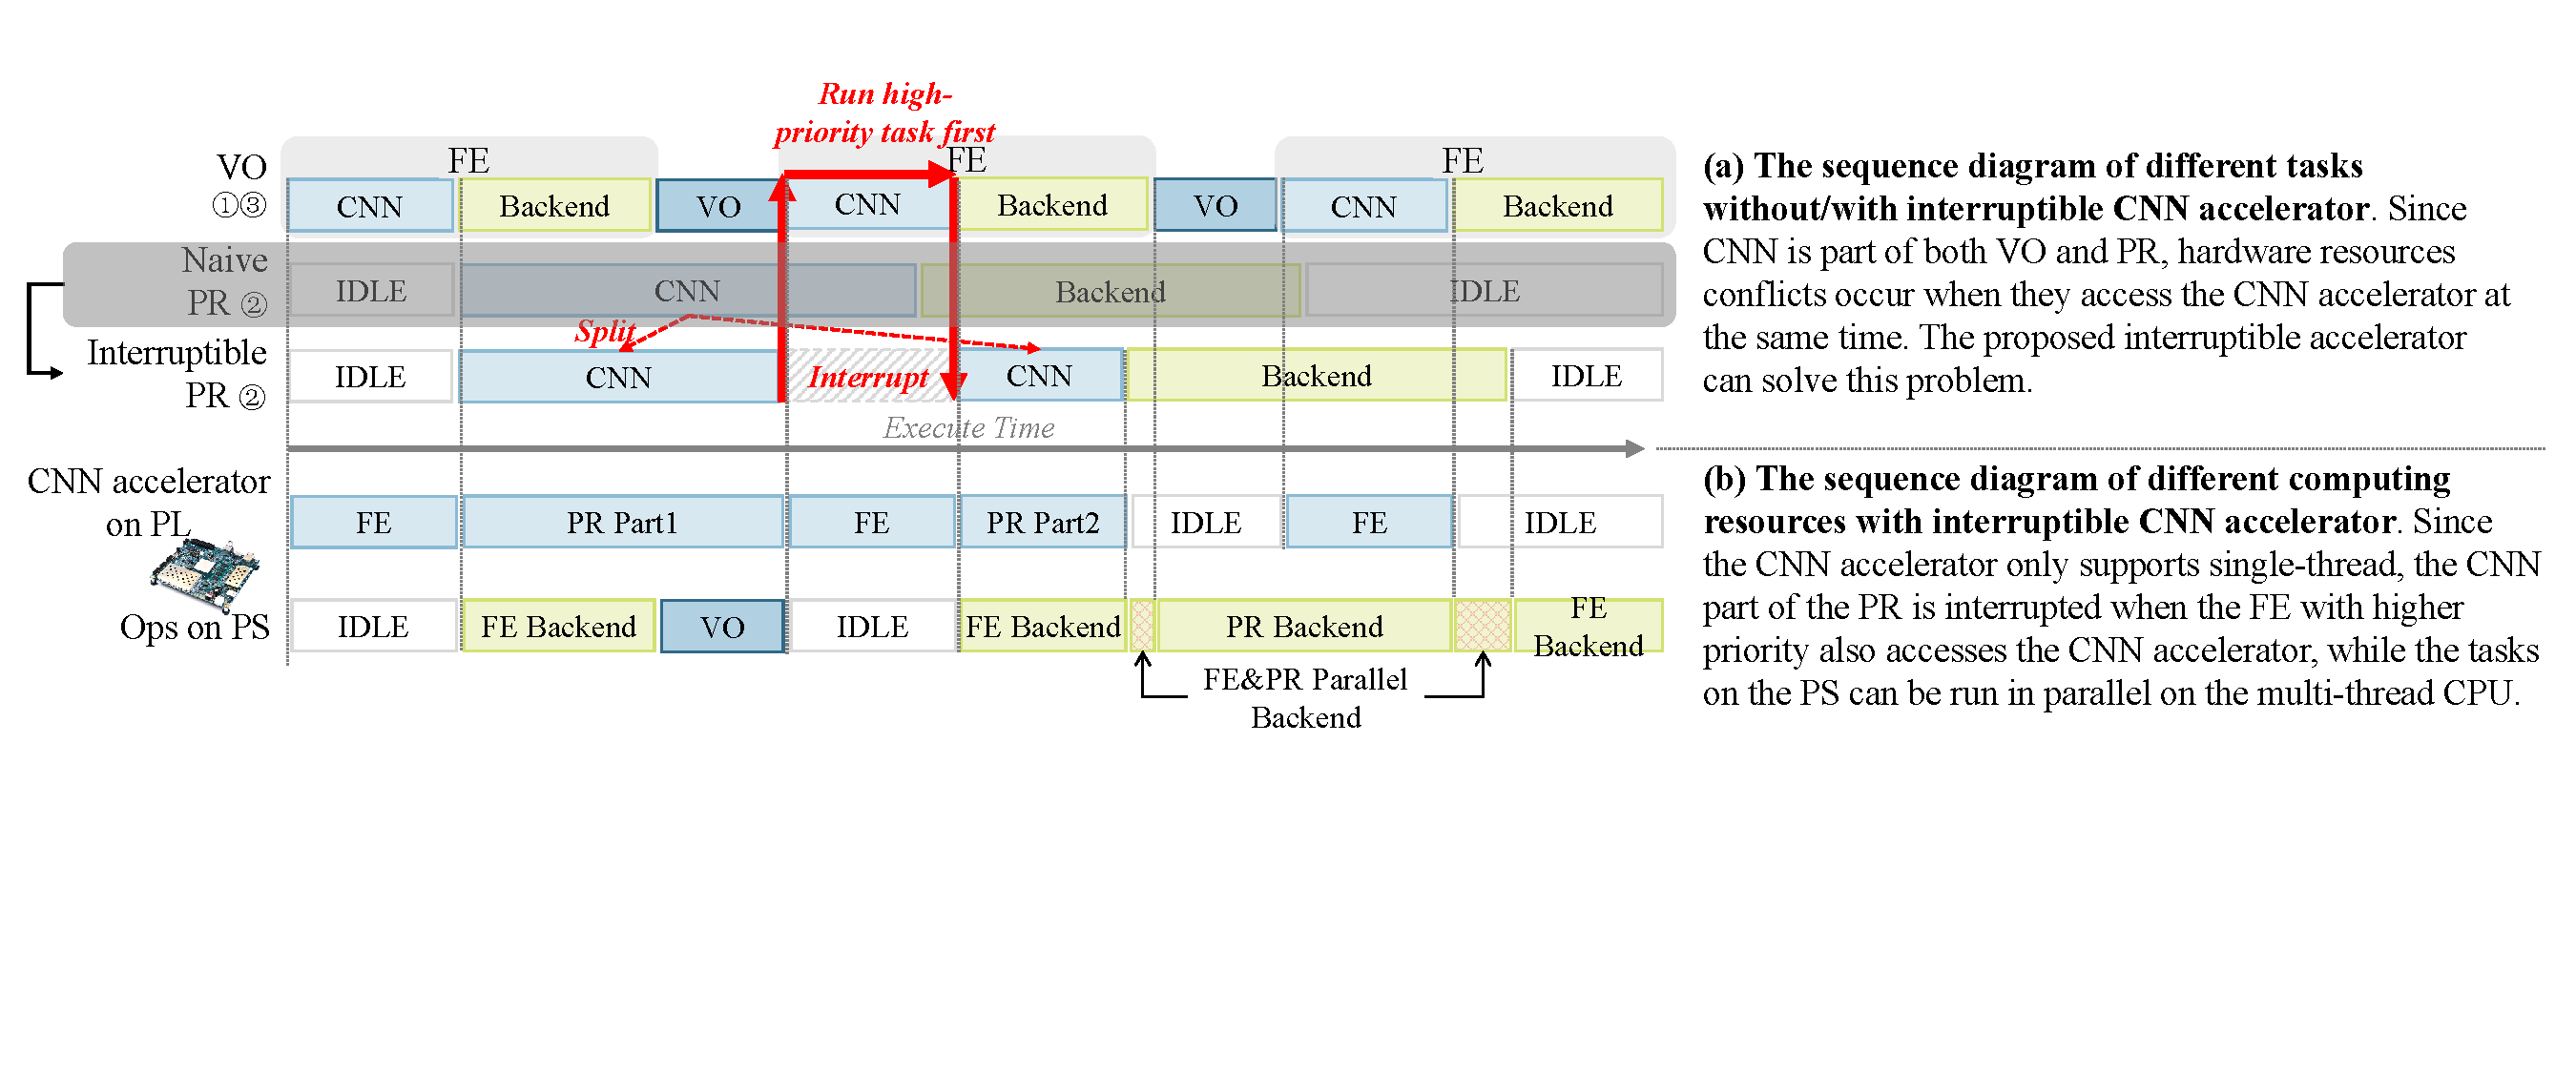
\includegraphics[width=0.95\linewidth]{fig/interDPR.pdf}
    \vspace{-2mm}
    \caption{Illustration of the accelerator interrupt to solve the hardware resources conflicts. When a high-priority task (FE) starts before the low-priority task (PR) completes, the CNN accelerator backs up the status of the low-priority task to the memory, and processes the high-priority task. When the high-priority task finishes, the low-priority task resumes and continues.
    }
	\label{fig:interDPR}
\end{figure*}


\subsection{ CNN-based FE and PR }

\textbf{Feature-point extraction:} Previous feature-point extraction works usually consist of two parts: 1) feature-point detection to find the positions of feature-points and 2) descriptor generation to describe the extracted feature-point with a code.
SIFT  ~\cite{Lowe-478}  detects and describes feature-points. The SIFT descriptor is rotation and scale invariant, so that the relative pose transformation between input images via matching SIFT feature-points is accurate. However, the computation of SIFT is complicated and slow  ~\cite{bay2006surf}. Thus, some other handcrafted methods, such as SURF ~\cite{bay2006surf} and ORB  ~\cite{Mur-Artal:2017281}, are proposed as fast alternatives to SIFT. ORB  ~\cite{Mur-Artal:2017281} method is widely used for its balance between speed and accuracy.
Recently, CNN is used to extract feature-points.  ~\cite{simo2015discriminative} proposes a CNN-based descriptor generator that exceeds ORB in accuracy.
SuperPoint  ~\cite{detone2018superpoint} presents a fully CNN-based feature-point extraction method that implements feature-point detection and descriptor generation using one CNN network. SuperPoint ~\cite{detone2018superpoint} reaches 10\%-30\% higher matching accuracy compared with the ORB-based feature-point extraction  ~\cite{Mur-Artal:2017281}. 
% SuperPoint is used in this work.

\textbf{Place recognition:} Before CNN-based place recognition, Bag of Words (BoW)  ~\cite{small_1} relying on handcrafted features is the most popular method. The accuracy of BoW-based methods is strongly influenced by the codebook size (descriptor length). Larger codebooks (1MB $\sim$ 10MB)  ~\cite{large_1, large_2} can compete with CNN-based methods in accuracy. However, they take up huge storage and communication resources. Smaller codebooks ~\cite{small_1, small_2, jegou2014triang} require less space but get worse accuracy. In contrast to traditional methods, CNN-based methods not only perform well but also generate more compact features, saving storage and communication resources. GeM  ~\cite{radenovic2018fine} and NetVLAD  ~\cite{arandjelovic2016netvlad} are popular CNN-based methods for their accuracy and data efficiency. GeM  ~\cite{radenovic2018fine} is 20\% better than the handcrafted method rootSIFT  ~\cite{jegou2014triang}.

Due to the advantage of CNN in image-based tasks, more and more CNN-based methods are used in the robotic system.


\subsection{ FPGA accelerators for a specific robot task }

The feature-point extraction (FE) operation is the fundamental component of a vision based robot, and is also one of the most time-consuming components  ~\cite{fang2017fpga}.
Some previous works design hardware architectures for FE.
SRI-SURF  ~\cite{jia2016sri} optimizes the memory access to speed up SURF  ~\cite{bay2006surf} feature-point extraction. 
~\cite{fang2017fpga} directly implements ORB on FPGA using HLS. eSLAM ~\cite{liu2019eslam} optimizes the ORB algorithm and designs hardware for better performance.
Some other works design architectures for the entire robot system. Hero  ~\cite{shi2018hero} is a framework for navigation and laser-based robot, which cannot support light-weight and cheap visual robots. 
~\cite{li2019879gops} introduces CNN accelerators for the vision-based robot. 
However, the CNN accelerator in that work ~\cite{li2019879gops} is only used for feature-point extraction, and the accelerator does not support different tasks at the same time. 
Deploying multiple CNNs on the robotic accelerator can expand the functions of robots, without designing hardware for specific functions.



\subsection{ CNN accelerators }
\textcolor{blue}{
FPGA is becoming a promising solution for CNN acceleration. 
Compared with CPU, GPU, and DSP platforms, for which the software and hardware are designed independently, FPGA eliminate the redundancy in general hardware platforms and achieve higher efficiency \cite{guo2019dl}.
Although Application Specific Integrated Circuits (ASICs) for CNN can achieve higher efficiency but require much longer devepoment cycle and higher cost. And once ASICs are taped out, it is difficult to add new hardware components to the produced ASICs.
For example, the hardware back-end for feature-point extraction, such as the hardware in \Cref{sec:hardsoftcodesign} is difficult to be added to a ASIC CNN accelerator.
}

To accelerate CNN on FPGA, some previous works design frameworks to generate a specific hardware architecture for a target CNN, based on  RTL  ~\cite{li_high_2016} or HLS  ~\cite{lu_evaluating_2017}. These works need to reconfigure the FPGA to switch between different CNN models. 
The reconfiguration takes seconds  ~\cite{FPGAPerformance}, which is unacceptable for the real-time system. 
\textcolor{blue}{
Although partially reconfiguration reprograms only part of the FPGA to reduce the reconfiguration time, high-performance design frameworks for FPGA ~\cite{li_high_2016,lu_evaluating_2017} jointly design and schedule the resources on the entire FPGA, which prevents reconfiguring FPGA from reprograming only a small number of hardware resources.
Thus, some work uses the CPU as the controller to dynamically configure and schedule the FPGA accelerator ~\cite{meloni2018neuraghe}.
}
Some other works design instruction-driven accelerators  ~\cite{gokhale2017snowflake,yu2018instruction,qiu2016going,guo2017angel,dpu}, which make rapid switching possible by providing different instruction sequences. 

However, the CNN tasks on previous instruction-driven CNN accelerators are not interruptible, resulting in the latency-sensitive high-priority task waiting for the low-priority task to finish. 
This inability of CNN accelerators to support multi-task makes it difficult for robotic researchers to use embedded FPGA. 
Furthermore, these accelerators are only designed for the uniformed operations of CNN backbones. It is also challenging to perform the post-processing in real time on the embedded CPU. 
Some previous works, such as HeteroCL \cite{lai2019heterocl}, provide programming paradigms and languages for both CNN backbones and post-processing. These hybrid programming platforms cannot support dynamic multi-task scheduling, and the performance is not as good as the specially designed CNN accelerators. 

% However, previous instruction-driven CNN accelerators need to schedule the entire CNN, and can not automatically schedule two or more tasks simultaneously. The inability of CNN accelerators to support multi-task makes it difficult for robotic researchers to use embedded FPGA.

\section{INCAME Framework}
\label{sec:incame}

To solve the hardware resources conflicts when the ROS software accesses the CNN accelerator, we propose the INCAME framework in this section.



\begin{figure}[t]
	\centering
    % \vspace{-0.1cm} 
    % \setlength{\abovecaptionskip}{0.cm} 
    % \setlength{\belowcaptionskip}{-0.25cm} 
    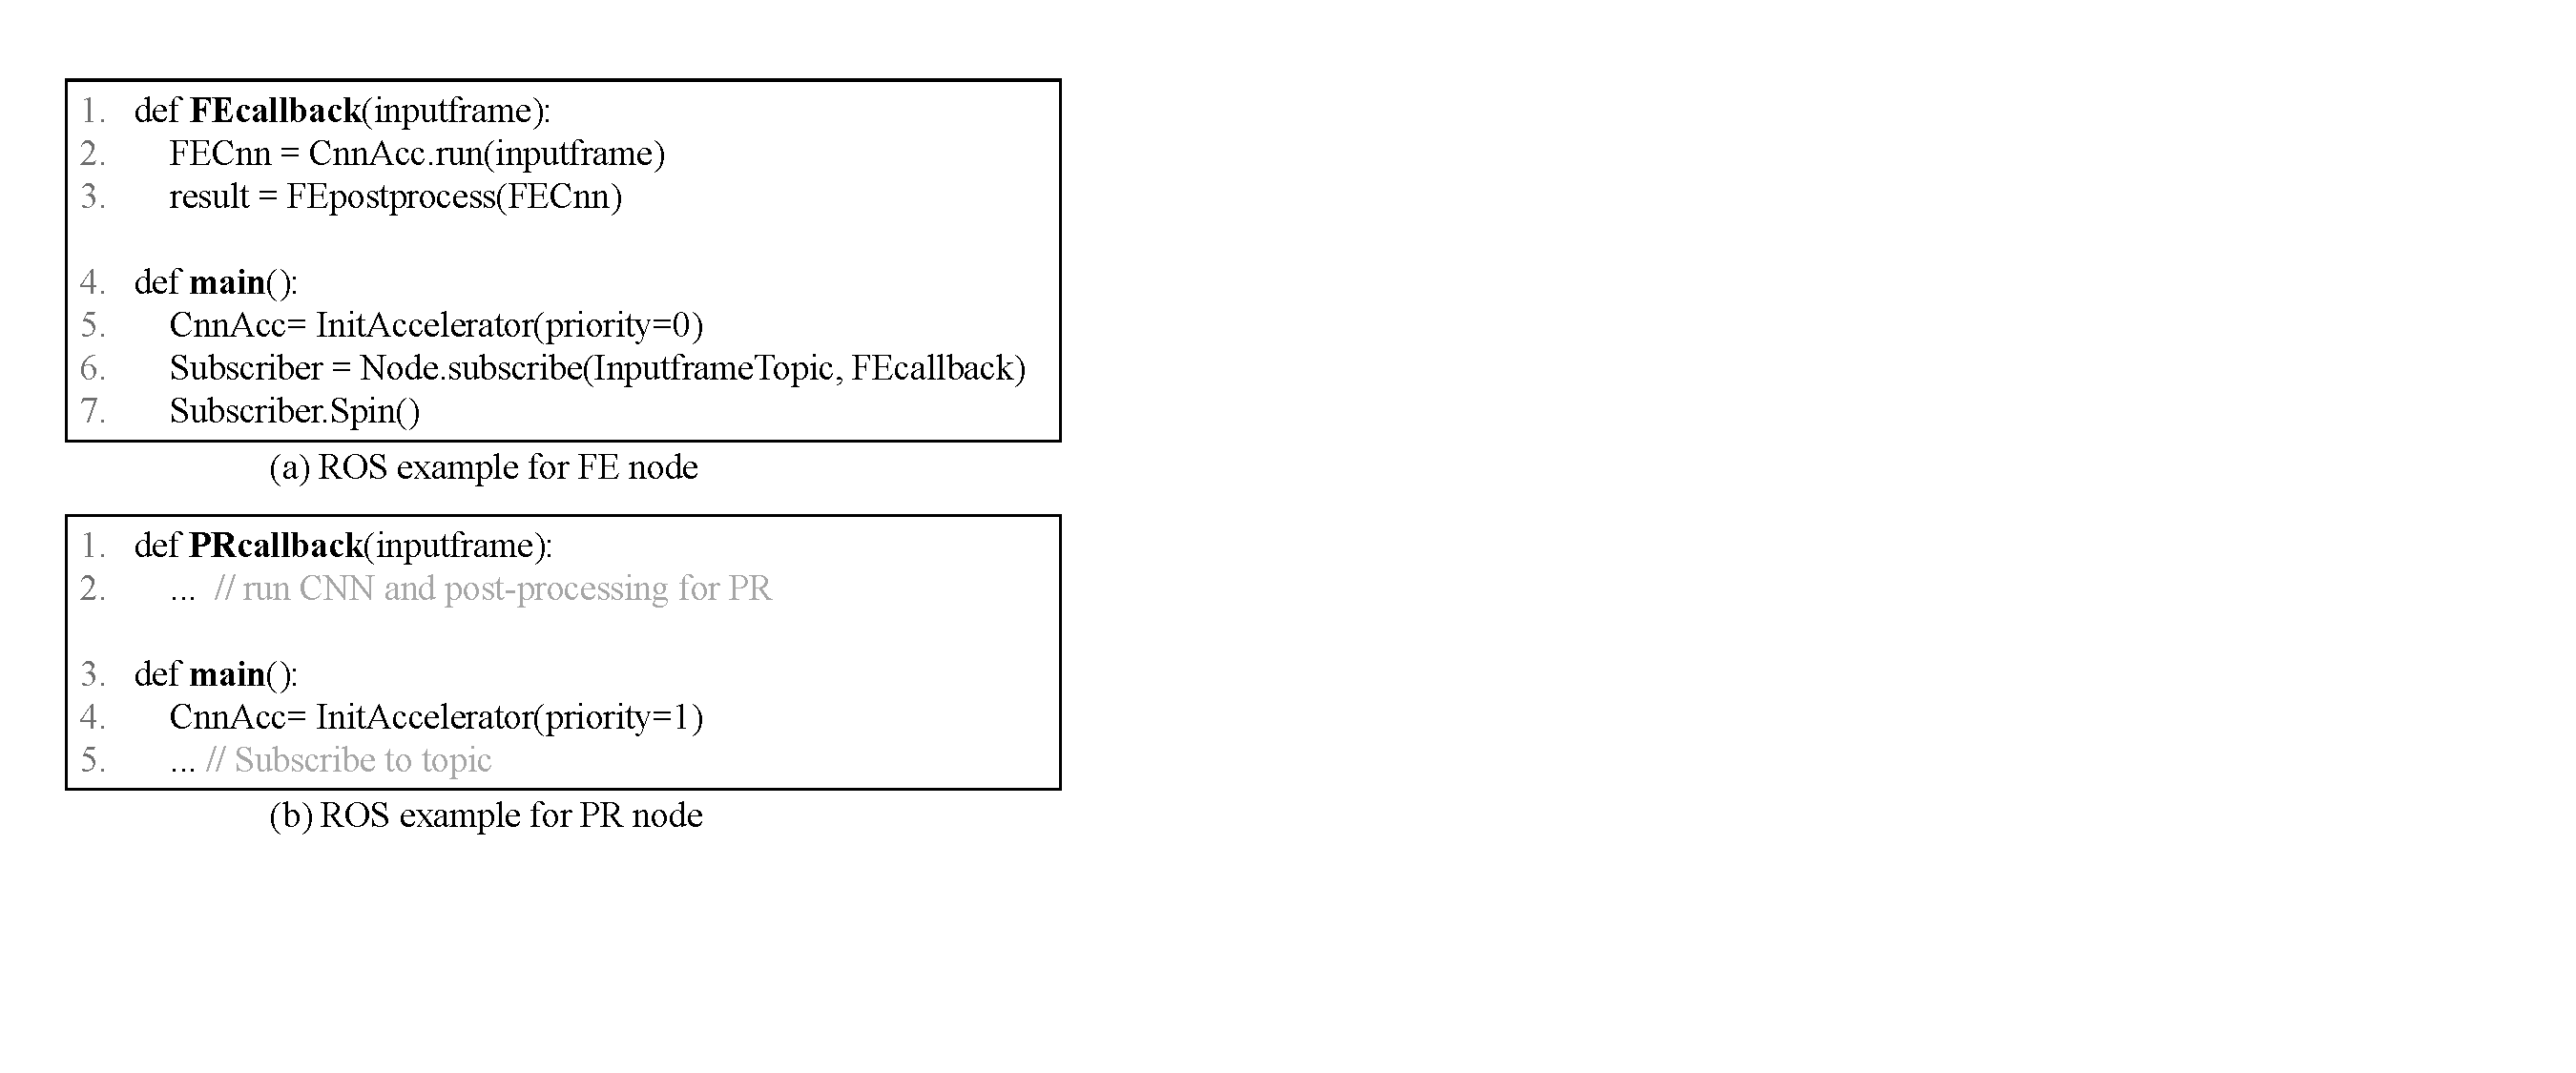
\includegraphics[width=0.9\linewidth]{fig/codeexample.pdf}
    \caption{ ROS code examples.}
	\label{fig:rosexample}
\end{figure}

\begin{figure*}[t]
	\centering
    % \vspace{-0.1cm} 
    % \setlength{\abovecaptionskip}{0cm} 
    % \setlength{\belowcaptionskip}{-0.05cm} 
    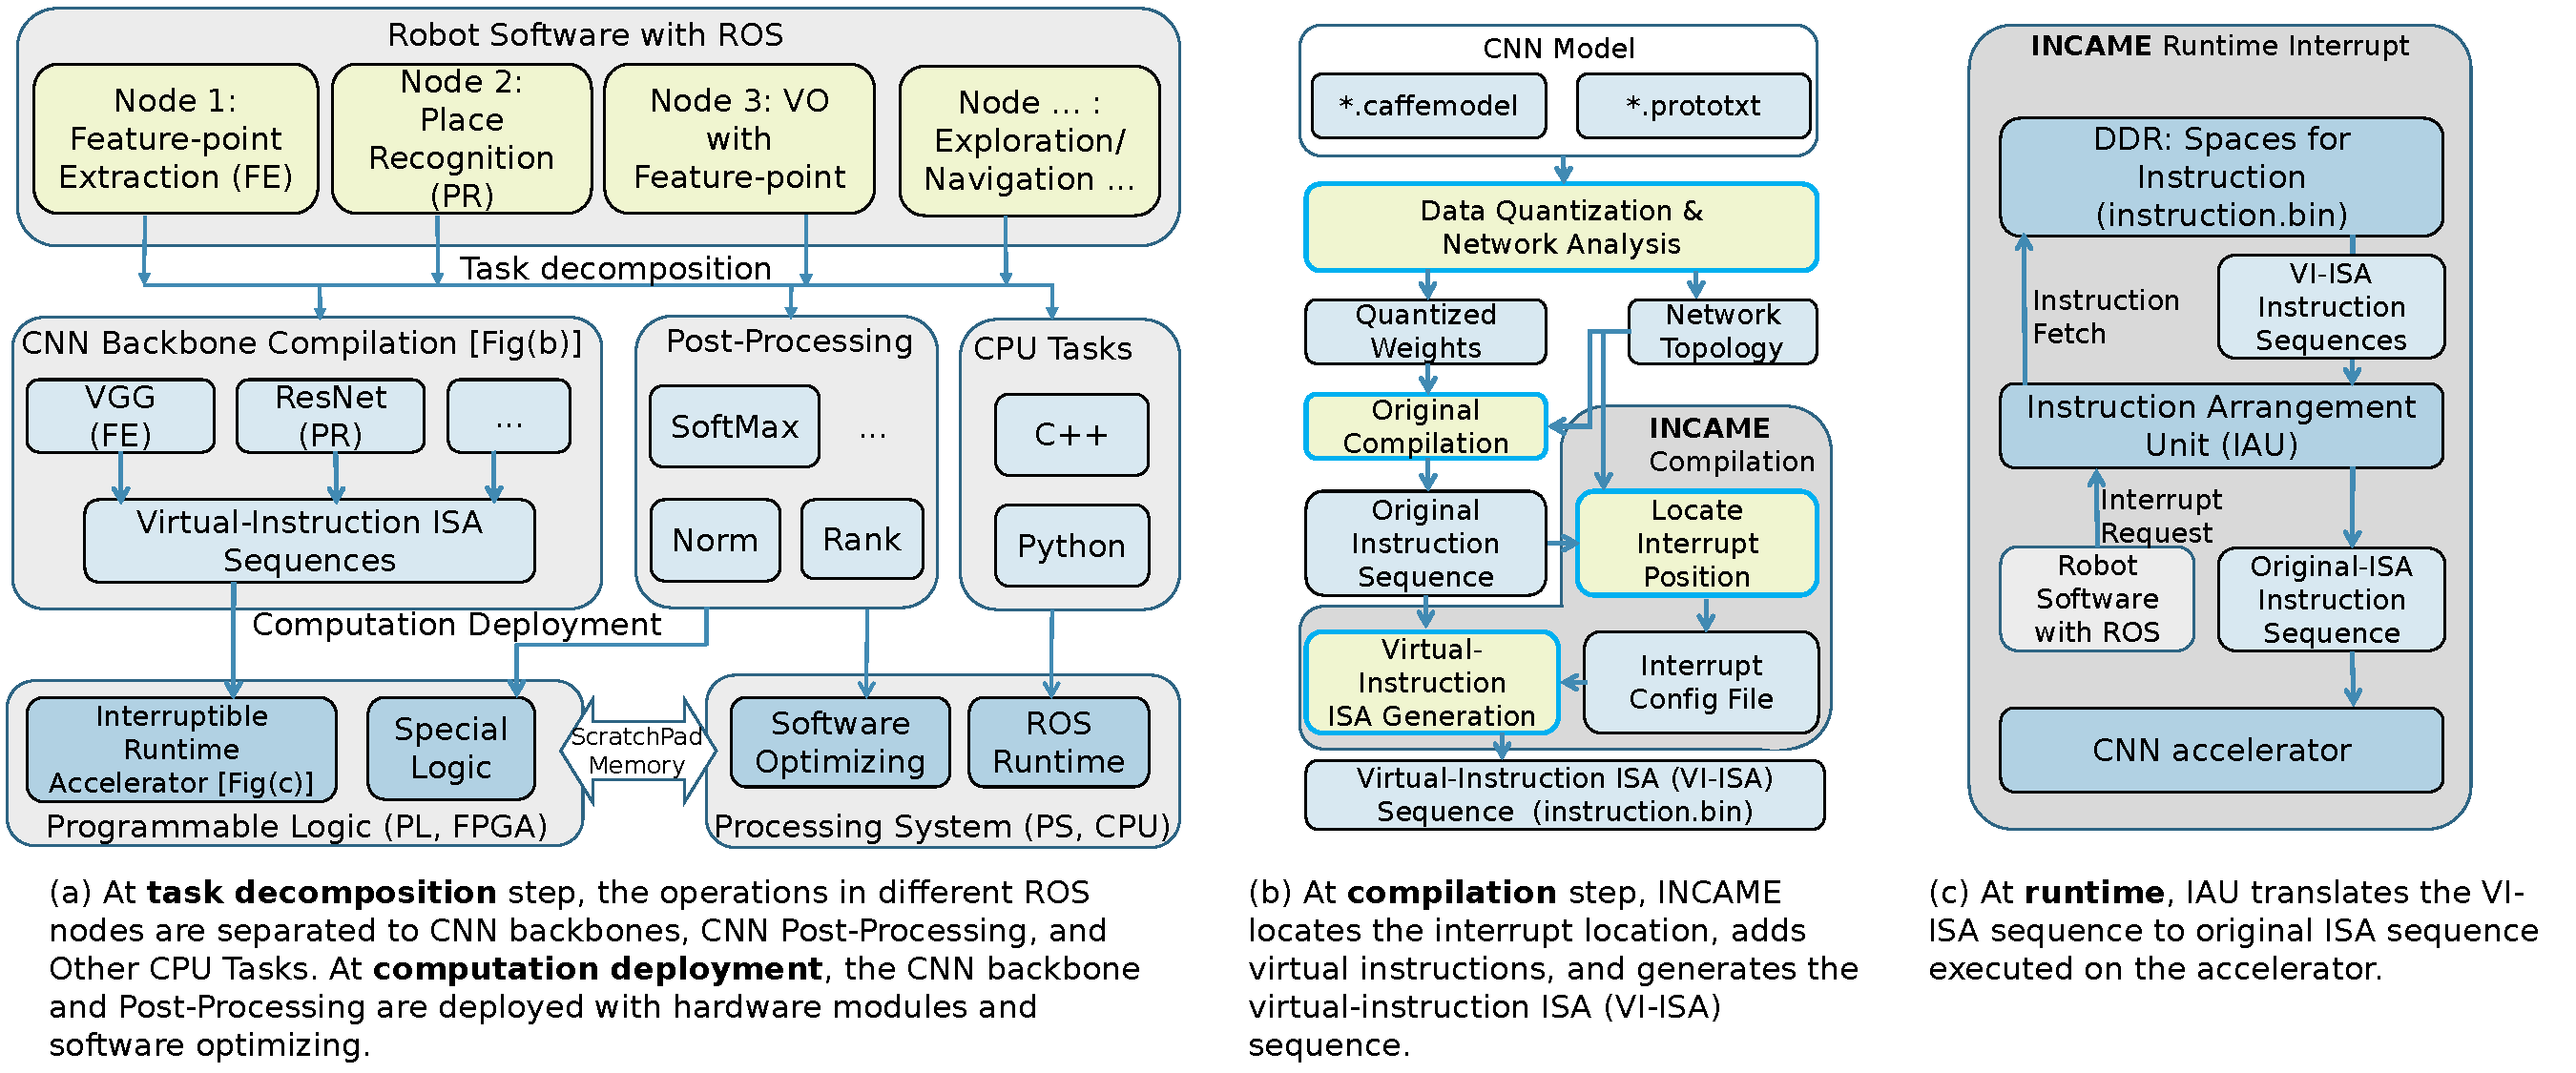
\includegraphics[width=0.99\linewidth]{fig/incame.pdf}
    \caption{ INCAME framework.}
	\label{fig:incame}
\end{figure*}

\subsection{Hardware Resources Conflicts In ROS}
\subsubsection{Introduction to ROS} Building a real robot requires many different components, including sensors, perception algorithms, and control units from different developers. The Robot Operating System (ROS)  ~\cite{quigley2009ros} is proposed to fuse the components from different researchers into a real system.
%  ROS is a popular framework for developing a robot, which provides programming specifications and a communication interface.

Each function module, such as FE, PR, and VO, is called a \textbf{Node} in ROS. Each node is an independent thread running on CPU, and does not know the running status of others. 
% Different nodes communicate with others by \textbf{ROS topics}. 
A node can publish \textbf{ROS topics} and subscribe to topics. The publishing and subscribing nodes connect to the same topic.
% , and neither node needs to know whether the other exists.
The subscribing node processes the received topics with callback functions. Line 6,7 in \Cref{fig:rosexample}(a) bind the topics (InputFrame) with the callback function (FEcallback to extract the feature-points). 


% The publishing node is called publisher, the subscribing node is called subscriber.

% \textbf{Publisher.} When the output of a publisher node is ready, the output data are inmediately packaged to the topic and published. ROS provides some system publisher, such as cv\_camera  ~\cite{cvcamera} to read the camera and publish the input frames to a ROS topic.

% \textbf{Subscriber.} The subscriber processes received topics through \textbf{callback} functions. Each callback function is bound to a topic. When the topic receives data, the callback function executed to process the data. If the callback function cannot complete before receiving the new data, the newly received data will be discarded.


 

% \subsection{Hardware Resources Conflicts in ROS}

\subsubsection{Hardware Resources Conflicts In ROS} Although ROS is becoming the fundamental software platform for robotics, the independence between different ROS nodes brings \textbf{hardware resources conflicts challenge} to access the hardware accelerator. 
% Because developers cannot predict the running state of the CNN accelerator when they write programs, the accelerator may be occupied by other threads when a ROS node needs to call the accelerator. 
\Cref{fig:rosexample}(a) Line 5 and \Cref{fig:rosexample}(b) Line 4 initialize the accelerator for the nodes. Line 2 in \Cref{fig:rosexample}(a) (b) runs the CNN backbone on the accelerator, respectively. Different nodes in ROS initialize and run the CNN accelerator independently, which may result in hardware resources conflicts. To address this problem, we set the priorities of different tasks at the initialization phase (the {\color{red}priority} parameter), and enable the accelerator interrupt to schedule the high-priority task firstly.

% The runtime status of the CNN accelerator is not predictable when developers writing the program. Line 13 in ROSExample1 and line 9 in ROSExample2 initialize the DPU for each task. Line5 in ROSExample1 an d line 3 in ROSExample2 run the tasks on the same CNN accelerator, which may result in hardware conflicts. In INCAME, the priorities of different tasks are configured at initialization phase to address the hardware conflicts problem.


% \begin{algorithm}[t]
%     \caption{ ROS Node for FE }
%     \label{code:FE}
%     \begin{algorithmic}[1]
%         \State {\color{gray} // imagePtr, imageAddr, fmPtr, fmAddr, DPUtask, Bankendtask  is initialized by main and used in FEcallback.}
%         \Function {FEcallback}{$ InputFrame $}
%         \State {\color{gray} // Read and reshape the InputFrame. }
%         \State {\color{blue} *imagePtr  $\gets$ *InputFrame }
%         \State DPUtask.run()
%         \State FEBackend.run()
%         \EndFunction

%         \Function {Main}{$ $}
%         \State {\color{gray} // Init ScratchPad Memory. Ptr is for CPU operations, Addr is for FPGA modules.}
%         \State imagePtr, imageAddr = ScratchPad(FEinputsize)
%         \State fmPtr, fmAddr = ScratchPad(FEfmsize)
%         \State {\color{gray}// Config task0 in IAU of the accelerator (DPU).}
%         \State DPUtask = DPUinit({\color{red}  priority=0},{\color{blue} instraddr=FEinstrAddr, }
%         \State \qquad \qquad \qquad \quad {\color{blue} inoffset=imageAddr,outoffset=fmAddr } ) 
%         \State FEBackend = FEBackendinit({\color{blue}fmAddr, fmPtr});
%         \State {\color{gray}// The node subscribes the inputframe, and use the FEcallback to process each inputframe.}
%         \State Subscriber = Node.subscribe( InputFrameTopic, FEcallback);
%         \State {\color{gray}// Use spin to start the subscriber}
%         \State Subscriber.spin();
%         \EndFunction
%     \end{algorithmic}
% \end{algorithm}

% \begin{algorithm}[t]
%     \caption{ ROS Node for PR }
%     \label{code:PR}
%     \begin{algorithmic}[1]
%         \Function {PRcallback}{$ InputKeyFrame $}
%         \State {\color{blue} *imagePtr  $\gets$ *InputKeyFrame }
%         \State DPUtask.run()
%         \State PRBackend.run()
%         \EndFunction

%         \Function {Main}{$ $}
%         \State imagePtr, imageAddr = ScratchPad(PRinputsize)
%         \State fmPtr, fmAddr = ScratchPad(PRfmsize)
%         \State DPUtask = PR\_DPUinit( {\color{red} priority=1},{\color{blue} instraddr=PRinstrAddr}, 
%         \State \qquad \qquad \qquad \quad {\color{blue} inoffset=imageAddr,outoffset=fmAddr } ) 
%         \State PRBackend = PRBackendinit({\color{blue}fmAddr, fmPtr});
%         \State Subscriber = Node.subscribe( InputKeyFrameTopic, PRcallback);
%         \State Subscriber.spin();
%         \EndFunction
%     \end{algorithmic}
% \end{algorithm}

% \subsection{ Accelerator interrupt to solve Hardware Resources Conflicts }

% In order to support multi-task scheduling and solve the hardware resources conflicts, interrupt is introduced to CPU  ~\cite{jen1974processor}. In this paper, we also use the concept of interrupt to support multi-task on the CNN accelerator.


% If the CNN accelerator supports interrupt, it can run two or more CNN modules at the same time. 
\subsubsection{Accelerator interrupt} \Cref{fig:interDPR} illustrates the idea of interrupt to schedule two CNN tasks. In the process of running a low-priority network (PR), the software may send an execution request for the high-priority task (FE). The interrupt enables the CNN accelerator to backup the running state of the low-priority PR network. Then the accelerator switches to the high-priority FE network. After the high-priority task (FE) completes, the low-priority task (PR) is restored to the accelerator and continues to execute.
% With the help of accelerator interrupt, the execution of the low-priority task (PR) is divided into pieces, and each piece is allocated to the time interval of running different high-priority networks (FE). 
% Accelerator interrupt multiplexes the time division of the accelerator, reduces the idle time of the accelerator, and improves the utilization of hardware resources. 





\subsection{ Interruptible Accelerator with ROS (INCAME) }

% We try to use CNN as much as possible to accomplish various tasks on the robot. Because the CNN not only has advantages over traditional algorithms in accuracy, but also has uniform and regular computing mode. Therefore, a single instruction-driven CNN accelerator can speed up different tasks. The unified accelerator can reduce the use of hardware resources and make it easier to implement the robot computing system on embedded FPGA.

\Cref{fig:incame}(a) illustrates the proposed two-step INCAME framework for mapping ROS based software to embedded FPGA.
The first step is the task decomposition, which decomposes the computation in ROS nodes into different INCAME computation types, including CNN backbones, CNN post-processing, and other CPU tasks. 

The second step is to deploy the computation onto the FPGA. 
The CNN backbones of different tasks, such as the VGG model  ~\cite{kim2016accurate} in SupoerPoint feature-point extraction  ~\cite{detone2018superpoint} and the ResNet101 model  ~\cite{he2016deep} in GeM place recognition  ~\cite{radenovic2018fine}, are compiled to the interruptible Virtual-Instruction Instruction Set Architecture (VI-ISA), which runs on the CNN accelerator. The VI-ISA is a simple extension of the original ISA, in which the extension method is not limited to a specific original ISA. Thus, the virtual-instruction-based interrupt can be easily applied to various instruction-based CNN accelerators  ~\cite{yu2018instruction,qiu2016going}, such as Angel-Eye ~\cite{guo2017angel} and DPU ~\cite{dpu}.
% At runtime, the interruptible CNN accelerator runs these instructions to calculate the CNN backbones.
% To accelerate the post-processing operations of the CNN based methods, 

Hardware modules are implemented for the CPU-intensive Softmax  \cite{Softmax-wiki} and Normalization  \cite{Norm}. Some task-related software optimizations, such as Ranking and Non-Maximum Suppression (NMS)  \cite{NeubeckGool-NMS}, as well as other ROS tasks written in C++/Python, are processed on the CPU side.

To eliminate the memory copy between CPU cores and CNN accelerators, we use low-latency ScratchPad memory  \cite{Banakar2002Scratchpad} to directly feed the results from CNN backbones to the post-processing modules. 

\Cref{fig:incame}(b) details the INCAME compilation step and runtime interrupt. Caffe  ~\cite{jia2014caffe} is a popular software framework for CNN, and the *.caffemodel/*.prototxt files define the network parameters and structure in Caffe. The previous deployment process, such as Angel-Eye  ~\cite{guo2017angel} and DPU ~\cite{dpu}, quantizes the weights, and analyze the network topology. The original compiler translates the network topology and the quantization information into the original ISA sequence. INCAME goes further than previous CNN compilers. It selects the optimized interrupt positions in the original instruction sequence, and adds virtual instructions at these positions to enable accelerator interrupt. After that, the original instruction sequence and the added virtual instructions are wrapped to the new interruptible VI-ISA. The wrapped VI-ISA instructions are dumped into a file (instruction.bin), and can be loaded into the instruction spaces on FPGA's DDR.


As illustrated in \Cref{fig:incame}(c), at runtime, an Instruction Arrangement Unit (IAU) in hardware listens to the interrupt request from ROS software, fetches the corresponding VI-ISA interruptible instructions and translates them to the original ISA executed on the CNN accelerator in Angel-Eye  ~\cite{guo2017angel}. 
The detail of the Virtual-Instruction ISA (VI-ISA) and instruction arrangement unit (IAU) is introduced in \Cref{sec:cnninterrupt}. Although INCAME can be applied to various instruction-based CNN accelerators, we implement and evaluate it based on Angel-Eye  ~\cite{guo2017angel}.



\section{Virtual-instruction-based Accelerator Interrupt}
\label{sec:cnninterrupt}
% The idea of interruption is introduced for dynamic multi-task scheduling. This section details the implementation of our \textbf{Virtual instruction Interruption}. \Cref{fig:interDPR} illustrates the idea of interruption to full utilize the hardware resources.


% \begin{figure*}[t]
% 	\centering
% 	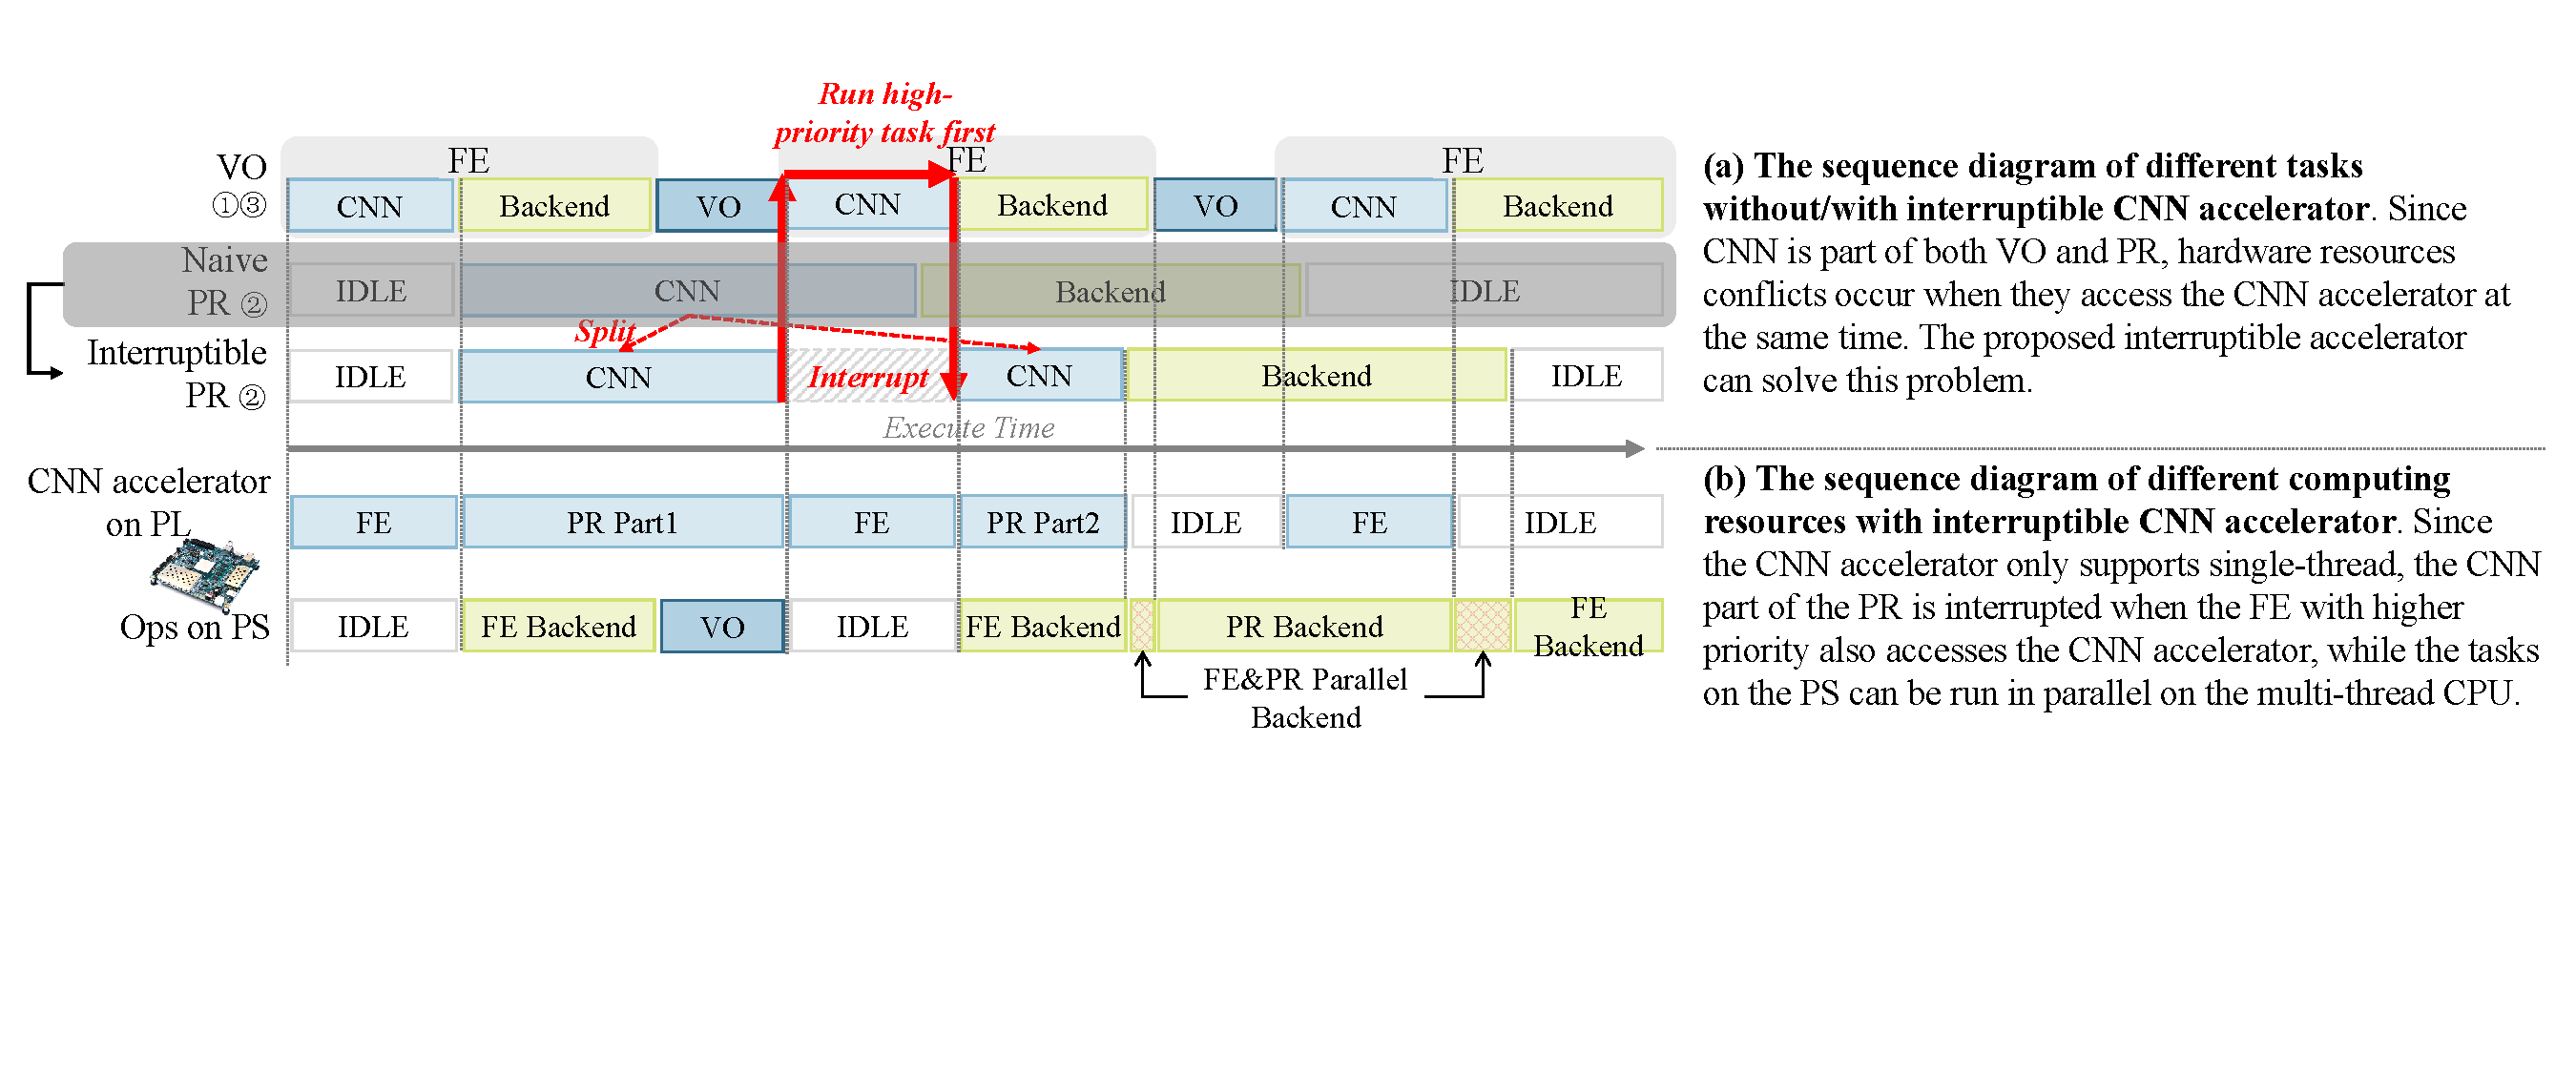
\includegraphics[width=0.99\linewidth]{fig/interDPR.eps}
% 	\caption{Interruption to solve the hardware resources conflicts.  When a high-priority task (FE) is started before the low-priority task (PR) is completed, the CNN accelerator backs up the status of PR to memory, and processes the FE task. When the high-priority task is completed, the low-priority task resumes and continues.
%     }
% 	\label{fig:interDPR}
% \end{figure*}


\begin{table*}[t]
	\caption{Description for the basic instructions.}
	\footnotesize
	\centering
% Table generated by Excel2LaTeX from sheet 'Sheet3'
%\linespread{1.1}\selectfont
\begin{tabular}{|p{2.7em}|m{3.7em}|m{14.2em}|m{4.2em}<{\centering}|m{4.2em}<{\centering}|m{4em}<{\centering}|m{4em}<{\centering}||m{6em}<{\centering}|m{6em}<{\centering}|}
	\hline
	\multicolumn{1}{|c|}{Category} & \multicolumn{1}{c|}{Type} & \multicolumn{1}{c|}{Description} & \multicolumn{1}{c|}{Address 1} & \multicolumn{1}{c|}{Address 2} & \multicolumn{1}{c|}{Address 3} & \multicolumn{1}{c||}{Workload} & \multicolumn{1}{c|}{Backup} & \multicolumn{1}{c|}{Recovery} \\
	\hline
	\multirow{2}[4]{*}{LOAD} & LOAD\_W & Load weights/bias from DDR to on chip weight buffer. & Off-chip Addr & Weights-buffer Addr & -     & Data  Length & -     & Weight / Inputdata \\
	\cline{2-9}\multicolumn{1}{|c|}{} & LOAD\_D & Load input data from DDR to on-chip data buffer. & Off-chip Addr & Data-buffer Addr & -     & Data  Length & -     & Weight / Inputdata \\
	\hline
	\multirow{2}[4]{*}{CALC} & CALC\_I & Calculate intermediate results (from partial input channels) for some output channels from partial  input channels. & Input  Data Addr & Intermediate Data Addr & Weight Addr & Calc Size & Previous final results / Intermediate data  & Weight / Inputdata /  Intermediate data \\
	\cline{2-9}\multicolumn{1}{|c|}{} & CALC\_F & Calculate the results for some output channels from all input channels. The pooling, bias-adding and element-wise operations are operated in this instructions. & Input  Data Addr & Output  Data Addr & Weight Addr & Calc Size & Final results & Inputdata \\
	\hline
	SAVE  & SAVE  & Save the results from on-chip data buffer to DDR. & Off-chip Addr & Data-buffer Addr & -     & Data  Length & -     & Inputdata \\
	\hline
	\end{tabular}%
	
	\label{tab:instr}%
  \end{table*}%


\begin{figure}[t]
	\centering
    % \vspace{-0.1cm} 
    % \setlength{\abovecaptionskip}{0cm} 
    % \setlength{\belowcaptionskip}{-0.6cm} 
	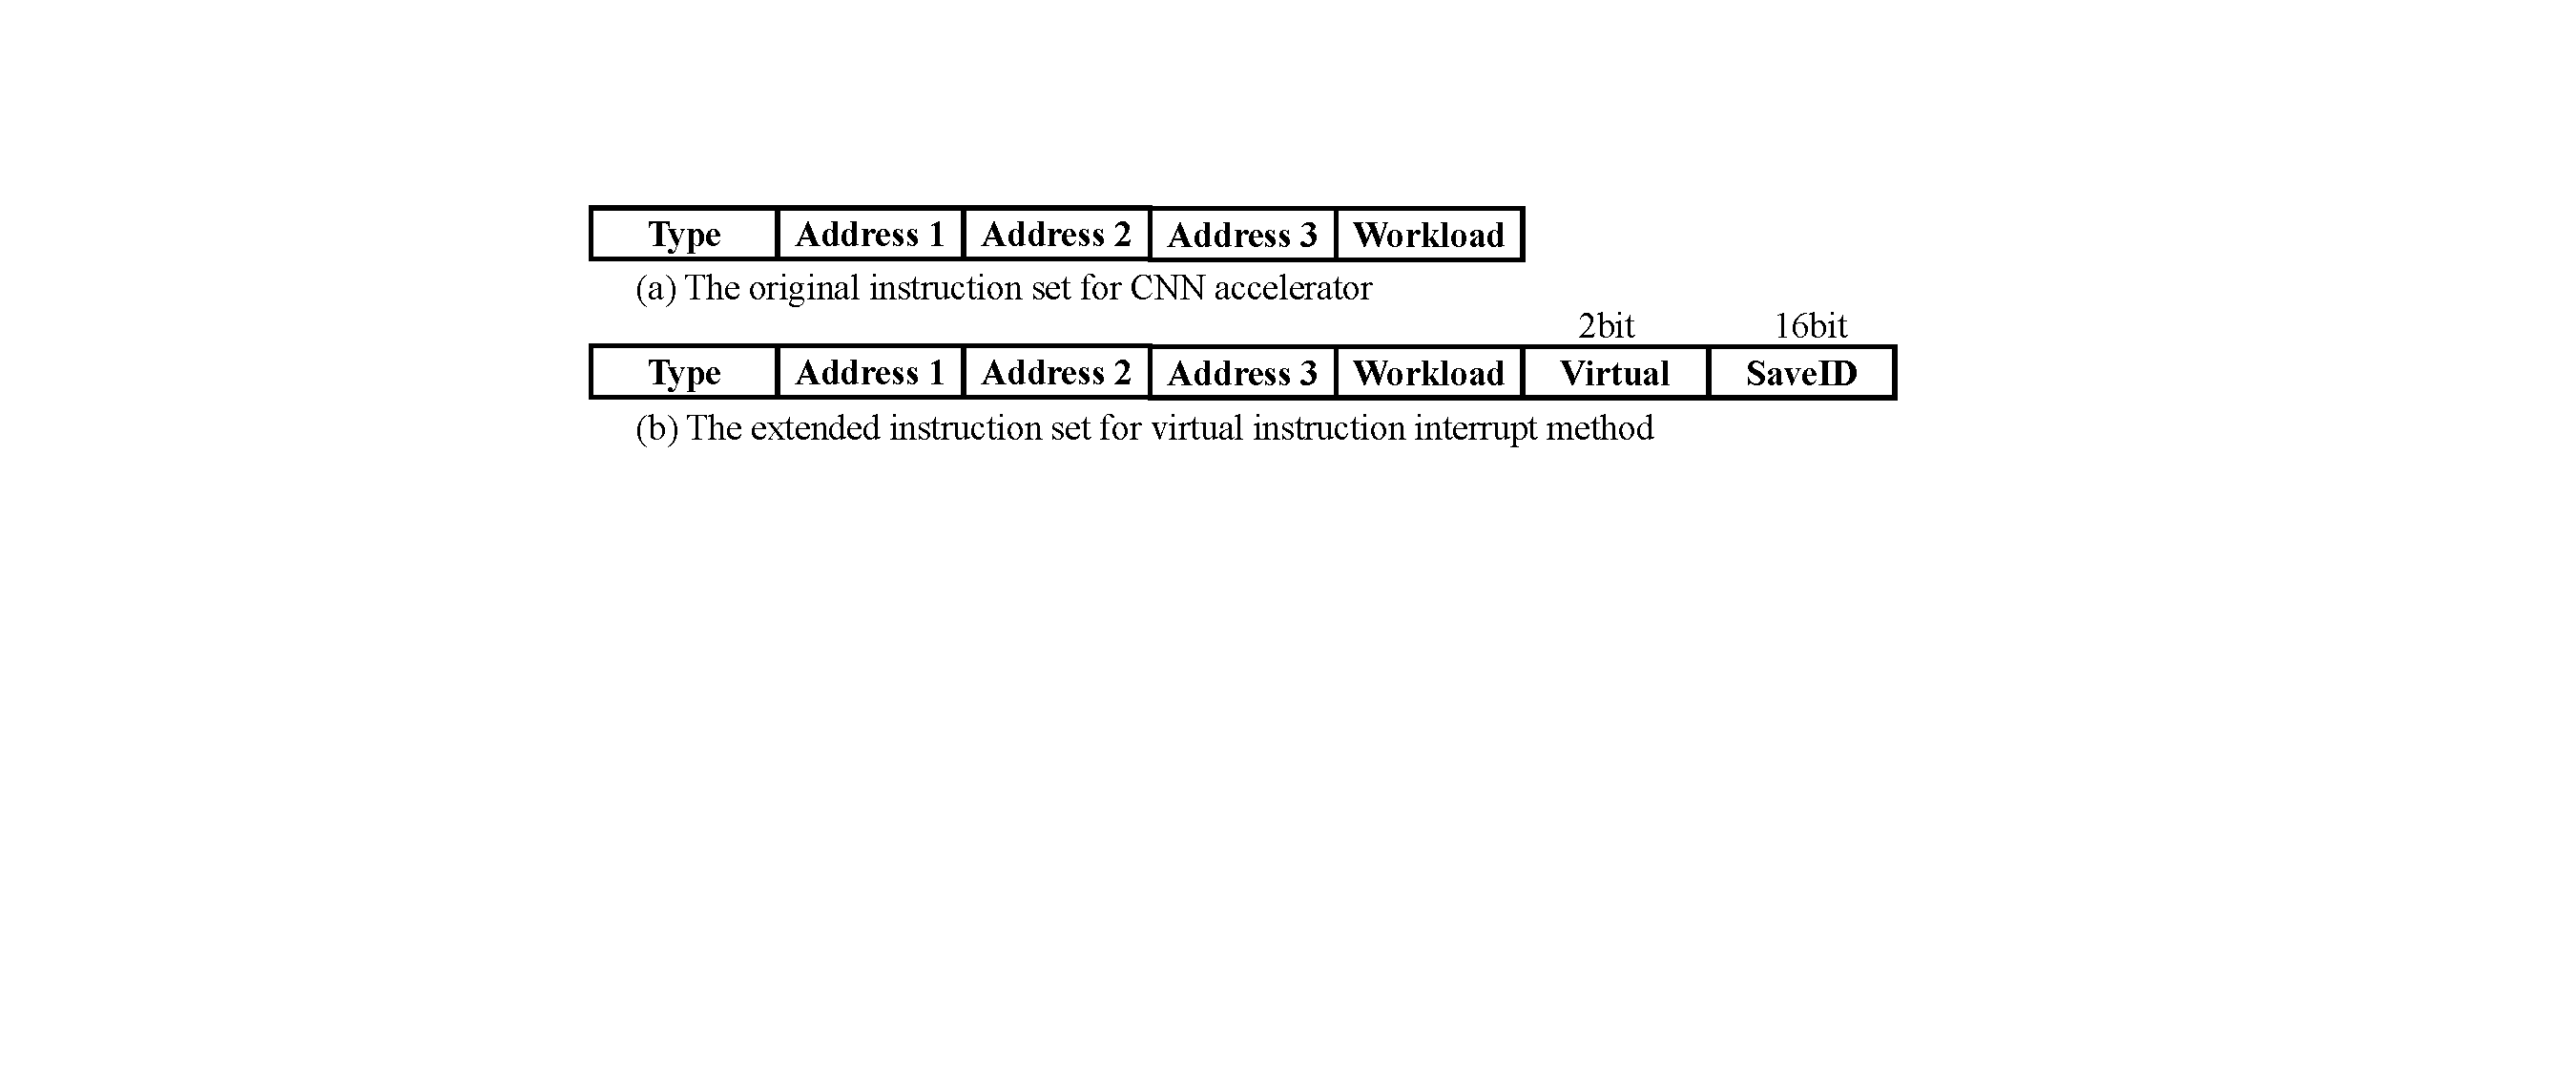
\includegraphics[width=0.99\linewidth]{fig/instructions.pdf}
	\vspace{-6mm}
	\caption{Fig(a), Original ISA. Fig(b), Virtual-Instruction ISA (VI-ISA).}
	\label{fig:instructions}
\end{figure}

In this section, we introduce our \textbf{virtual-instruction-based} method (VI method) to enable accelerator interrupt. Compared with the CPU-Like and Layer-by-Layer interrupt method, virtual-instruction-based method minimizes the interrupt response latency and the extra cost of the interrupt.
% In this section, we introduce our virtual-instruction-based method to enable accelerator interrupt. To minimize the interrupt response latency and extra cost for interrupt, we propose the virtual-instruction-based accelerator interrupt method.

\subsection{ Instruction Driven Accelerator }
\label{sec:instrAcc}
There are three categories of instruction in the instruction-driven accelerator: LOAD, CALC, and SAVE  ~\cite{guo2017angel,qiu2016going,yu2018instruction}. The instruction description of each kind of instruction is listed in \Cref{fig:instructions}(a) and \Cref{tab:instr}.

The LOAD instruction moves input featuremaps and weights from DDR to on-chip memory. The SAVE instruction moves the calculated output features from on-chip memory to DDR. 

Each CALC  instruction,  including CALC\_I and CALC\_F, processes the convolution according to the hardware parallelism with $Para_{height}$ lines from $ Para_{in} $ input channels to $ Para_{out}$ output channels. $Para_{height}$, $ Para_{in} $, and $ Para_{out} $ are the parallelism along the height, input channel and output channel dimensions, which is determined by the hardware and original ISA.

\Cref{fig:singlesave}(a) illustrates the operation of CALC instructions. The convolution of the last $ Para_{in} $ input channels is CALC\_F, and the convolutions for the former input channels are CALC\_I. The CALC\_F and the CALC\_I instructions for the same output channels, as well as the LOAD instructions for corresponding input featuremaps and weights, are considered as a \textbf{CalcBlob}  (\Cref{sec:exampleVirtual}(c) lists an example for CalcBlob). In each CalcBlob, there is a LOAD\_W instruction for the corresponding weights. However, as the input data can be shared across different CalcBlobs, some CalcBlobs do not have  LOAD\_D instruction. 

% Each CALC  instruction,  including CALC\_I and CALC\_F processes the convolution according to the hardware parallelism.
% Each CALC instruction, including CALC\_I and CALC\_F processes the convolution from input feature of the hardware input parallelism ($Para_{in}$) to the output feature of the hardware output parallelism ($ Para_{out}$), as illustrated in \Cref{fig:singlesave}(a). The convolution of the last input channels is CALC\_F, and the convolutions for the former input channels are CALC\_I. The CALC\_F and the CALC\_I instructions to generate the output channels, as well as the LOAD instructions for corresponding input featuremaps and weights are considered as a \textbf{CalcBlob}. Besides the convolution, some other operations like pooling is also represented in the CALC\_F instruction.

% Considerring to the limited on-chip data memory, the on-chip data buffer may not able to store all of the input and output featuremaps. To solve this problem, a CALC instruction is not designed for the entile featuremap, yet servel lines of the featuremap. The parallelism along the height dimension of a CALC instruction is denoted as  





% \subsection{Accelerator Interrupt }

\subsection{How To Interrupt: Virtual Instruction}
\label{sec:howinter}

As illustrated in \Cref{fig:singlesave}(e),there are four stages to handle interrupt, including: (1) Time for finishing the current operation, $t1$. (2) Time to backup, $t2$. (3) Time for the high-priority task, $t3$. (4) Time to restore the low-priority task ,$t4$. 
The latency to respond the interrupt is $t_{latency} = t_1+t_2$. The extra cost for interrupt is $t_{cost}=t_2+t_4$. For the instruction flow illustrated in \Cref{fig:singlesave}(c), the interrupt stages are shown in \Cref{fig:singlesave}(e).
There are different methods to implement interrupt in CNN accelerators.

\textbf{CPU-Like.}
When an interrupt request occurs in CPU, CPU backs up all the on-chip registers to DDR. However, there are only tens of registers in CPU, and the volume of the backed-up data is less than 1 KB  ~\cite{furber2000arm}. In CNN accelerators, there are hundreds of KB $\sim$ several MB on-chip caches  ~\cite{qiu2016going, guo2017angel} to store input featuremaps or weights. 
% If all on-chip caches are backed-up/recovered, the cost of data transfer in the accelerator is much higher than that of CPU. 
Thus, the extra data transfer increases both the interrupt response latency ($t_{latency}$) and the additional cost ($t_{cost}$).

\textbf{Layer-by-layer.}
Most accelerators run the CNN layer by layer  ~\cite{qiu2016going,guo2017angel}. 
There is no extra data transfer for the accelerator to switch between different tasks after each layer, thus, $t_{cost}=0$. 
However, the position of the interrupt request is irregular and unpredictable. When an interrupt occurs inside a CNN layer, the CNN accelerator needs to finish the whole layer before switching, which leads to the high response latency ($t_{latency}$).

% The latency to respond the interrupt and the performance degradation of the CPU-like interrupt and Layer-by-layer method will be evaluated in \Cref{sec:experiments}.



We propose the \textbf{virtual-instruction-based} method (VI method) to enable low-latency interrupt. 
% Different from the CPU-like interrupt, which backup/recovery all the on-chip caches, only the on-chip cache which is still needed in future execution will be backed-up and restored. So that the amount of data transfer is much lower than that of CPU-like interrupt.
To reduce the interrupt response latency, our virtual-instruction-based method is interruptible inside each layer. We add some virtual instructions to the original instruction sequence to enable the interrupt.
The virtual instructions, which contain the backup and recovery instructions, are responsible for backing up and restoring on-chip caches. 

\textbf{Virtual SAVE} instructions back up the intermediate results from partial input channels or the final output results. There is no need to back up the input featuremaps and weights, because these inputs are already stored in DDR. 

\textbf{Virtual LOAD} instructions restore the input featuremaps from DDR to on-chip caches.
% because input featuremaps are loaded by one CalcBlob, and shared across subsequent CalcBlobs, and thus the subsequent CalcBlobs do not read the input featuremaps. 
Virtual LOAD instructions also need to restore the intermediate results from partial input channels backed up by the virtual SAVE instructions.

% By adding the virtual instructions, the CNN can be interrupted anywhere, and the latency to respond interrupt is reduced.


% For backup virtual instructions, the corresponding input data and weights are already stored in DDR. 
% Thus, there is no need to back up the input buffer and weight buffer. Only the intermediate data and the final output results are needed to be backed-up. 

% For recovery virtual instructions, the weights and input data, as well as the backed-up intermediate data, are needed to be restored from DDR to the on-chip cache.
% The accelerator can switch to a different task after the backup virtual instructions, and resume the execution by the recovery virtual instructions.

% By adding the virtual instructions, the CNN can be interrupted anywhere, and the latency to to response the interrupt is reduced. However, there virtual instructions are only valid when interrupt occurs. So we add a field in the origin instruction set, that indicates whether the instruction a virtual instruction. If no interrupt occurs, virtual instructions will be skipped and discarded, which can ensure the efficiency of uninterrupted execution. The modifications to the instruction set will be introduced in \Cref{sec:virtualinstr}. 


% However, the CPU-like interrupt would back up all the on-chip registers to DDR. In CPU, there are tens of registers, and the backed-up data is around 1 KB. In CNN accelerators, there are hundreds of KB ~ several MB on-chip cache  ~\cite{qiu2016going, yu2018instruction}. If all the on-chip cache is backed-up and recovered, the cost of data transfer in the CNN accelerator is much higher than that of CPU.

% We propose the \textbf{virtual-instruction-based} method to enable low-latency interrupt. The low-priority task maintains the executing status itself, rather than the hardware or the interrupt handler used in CPU. Only the cache which is still needed in future execution will be backed-up and restored.

% The virtual instructions, which contain the backup and recovery instructions, are generated in the compilation phase, together with the normal instructions. 
% For backup instructions, the corresponding input data and weights are still stored in DDR. 
% There is no need to back up the input buffer and weight buffer, and only the intermediate data and the final output results are needed to be backed-up. 
% For recovery instructions, the weights and input data for future calculation, as well as the backed-up intermediate data, are needed to be restored from DDR to the on-chip cache.

% There is a field in the instruction set, that indicates whether the instruction a virtual instruction. If no interrupt occurs, virtual instructions will be skipped and discarded, which can ensure the efficiency of uninterrupted execution.







\begin{figure*}[t]
    % \flushleft
    \centering
    % \vspace{-0.1cm} 
    % \setlength{\abovecaptionskip}{0cm} 
    % \setlength{\belowcaptionskip}{-0.05cm} 
	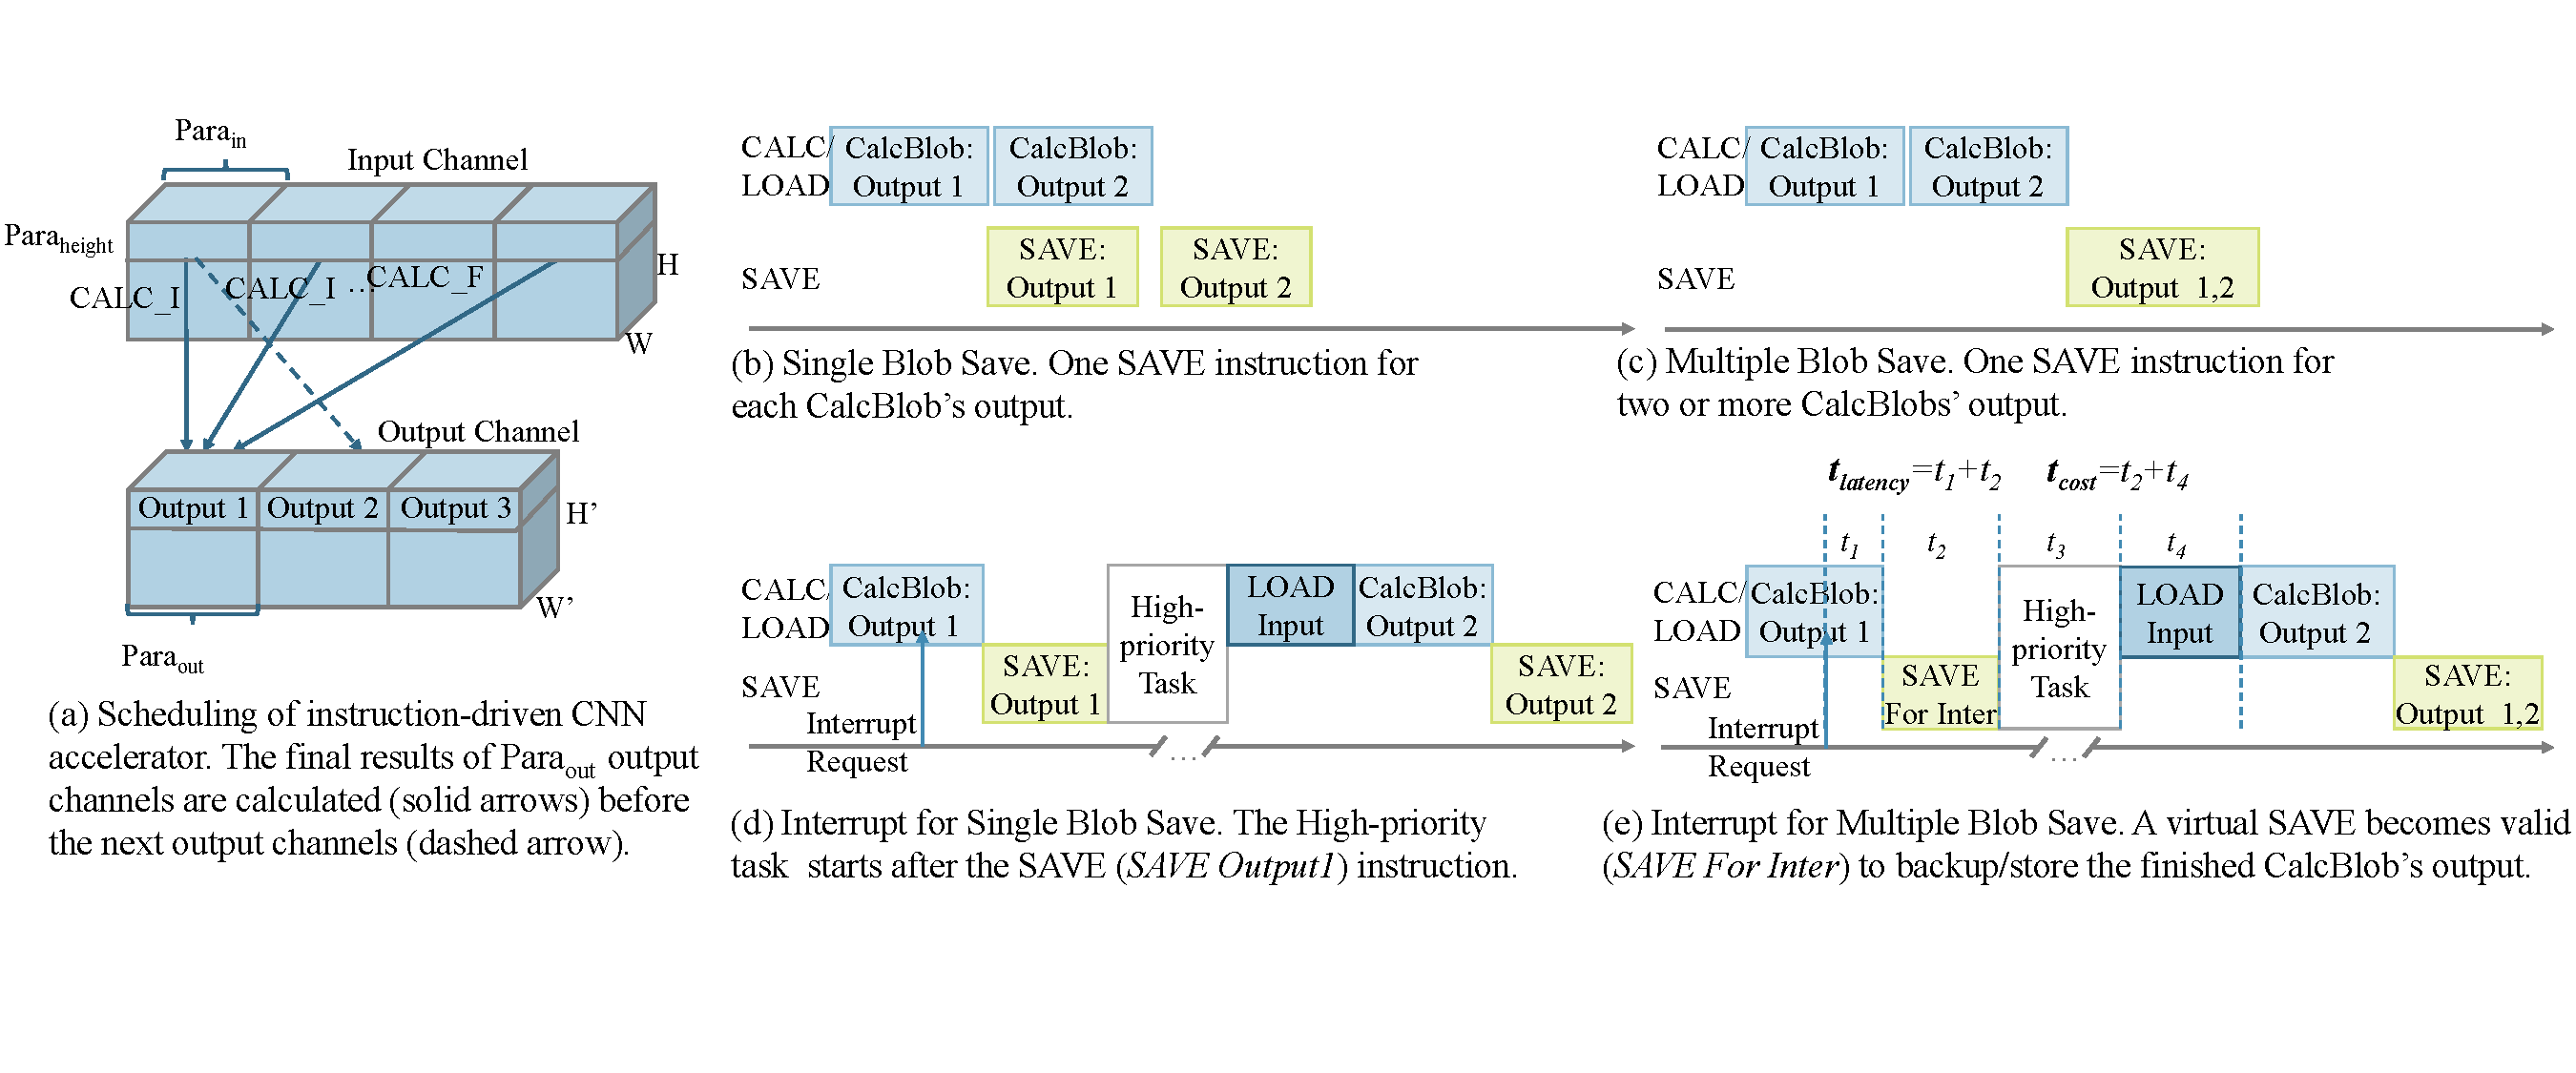
\includegraphics[width=0.99\textwidth]{fig/singlesave.pdf} 	
	\vspace{-1mm} 
    \caption{
		Illustration of scheduling on the CNN accelerator. Fig(a), a CalcBlob is the instructions that calculate the final results of $Para_{out}$ output channels from all input channels (the set of solid arrows). Fig(b), one SAVE instruction is only responsible for saving the results of one CalcBlob. Fig(c), one SAVE instruction is responsible for saving the results of several CalcBlobs. Fig(d) and Fig(e) illustrate the accelerator interrupt of Fig(b) and Fig(c). The latency($t_{latency}$) and extra cost ($t_{cost}$) are labelled in Fig(e).
    }
	\label{fig:singlesave}
\end{figure*}



\subsection{ Where To Interrupt: After SAVE/CALC\_F }
\label{sec:whereinter}
The virtual-instruction-based method has two potential factors that may lead to system performance degradation: 1) The extra data transfer to backup/restore running status takes up additional bandwidth resources. 2) The instruction fetching for the virtual instructions also uses bandwidth resources.
%  Even they are skipped and discarded.
To address the above problems of virtual-instruction-based method, we analyze the interrupt cost and select the positions of adding the virtual instructions.
The backup/recovery data for different interrupt positions at each kind of instruction are listed in the Backup/Recovery columns of \Cref{tab:instr}. The backup/recovery data transfer for each instruction is analyzed as follows:

\textbf{LOAD\_W / LOAD\_D. }
When an interruption occurs at LOAD, the newly loaded data are immediately flushed when running the high-level CNN, leading to bandwidth waste.

\textbf{CALC\_I.} 
When an interrupt occurs at CALC\_I, the unsaved final results (generated by previous CALC\_F) should be saved to DDR. The intermediate data from current CALC\_I should also be sent to DDR for further use. At the Recovery stage, the intermediate data should be fetched from DDR. The data movement of intermediate results leads to additional bandwidth requirements.


\textbf{CALC\_F.}
When an interrupt occurs at CALC\_F, there are no intermediate results. 
Although it is necessary to back up the unsaved final results which are generated by previous CALC\_F, these results will be stored in DDR through the subsequent original SAVE instruction.
If the accelerator can record the interrupt status, we can modify the address and workload when executing subsequent original not-virtual save instruction.
In this way, we can avoid the repetitive transmission of the final output results.
% The state records and modifications to normal SAVE instruction will be introduced in the following subsections.
The input data are shared across the CalcBlobs. Thus, the recovery virtual instruction needs to restore the shared input featuremaps.



\textbf{SAVE.}
The overhead of interrupt is only to transfer input data from DDR to the on-chip caches. 

In order to minimize the cost of interrupt, we make the CNN interruptible after the SAVE or CALC\_F. This method only introduces extra data transfer to recovery input data without any extra backup data ($t_2 = 0$). Thus, $t_{cost} = t_4$, in our virtual-instruction-based interrupt.

% Additional virtual instructions also take up bandwidth at instruction fetching phase, even if they are not executed. The instruction number of CALC\_I is tens of times of that of SAVE/CALC\_F. If the network can be interrupted after each CALC\_I, the rapidly increasing virtual instructions reduce the system performance.


\begin{figure*}[t]
	\centering
	\subfloat[$t_1$ for Layer-By-Layer method.]{
		\begin{minipage}[t]{0.45\linewidth}
			\centering
	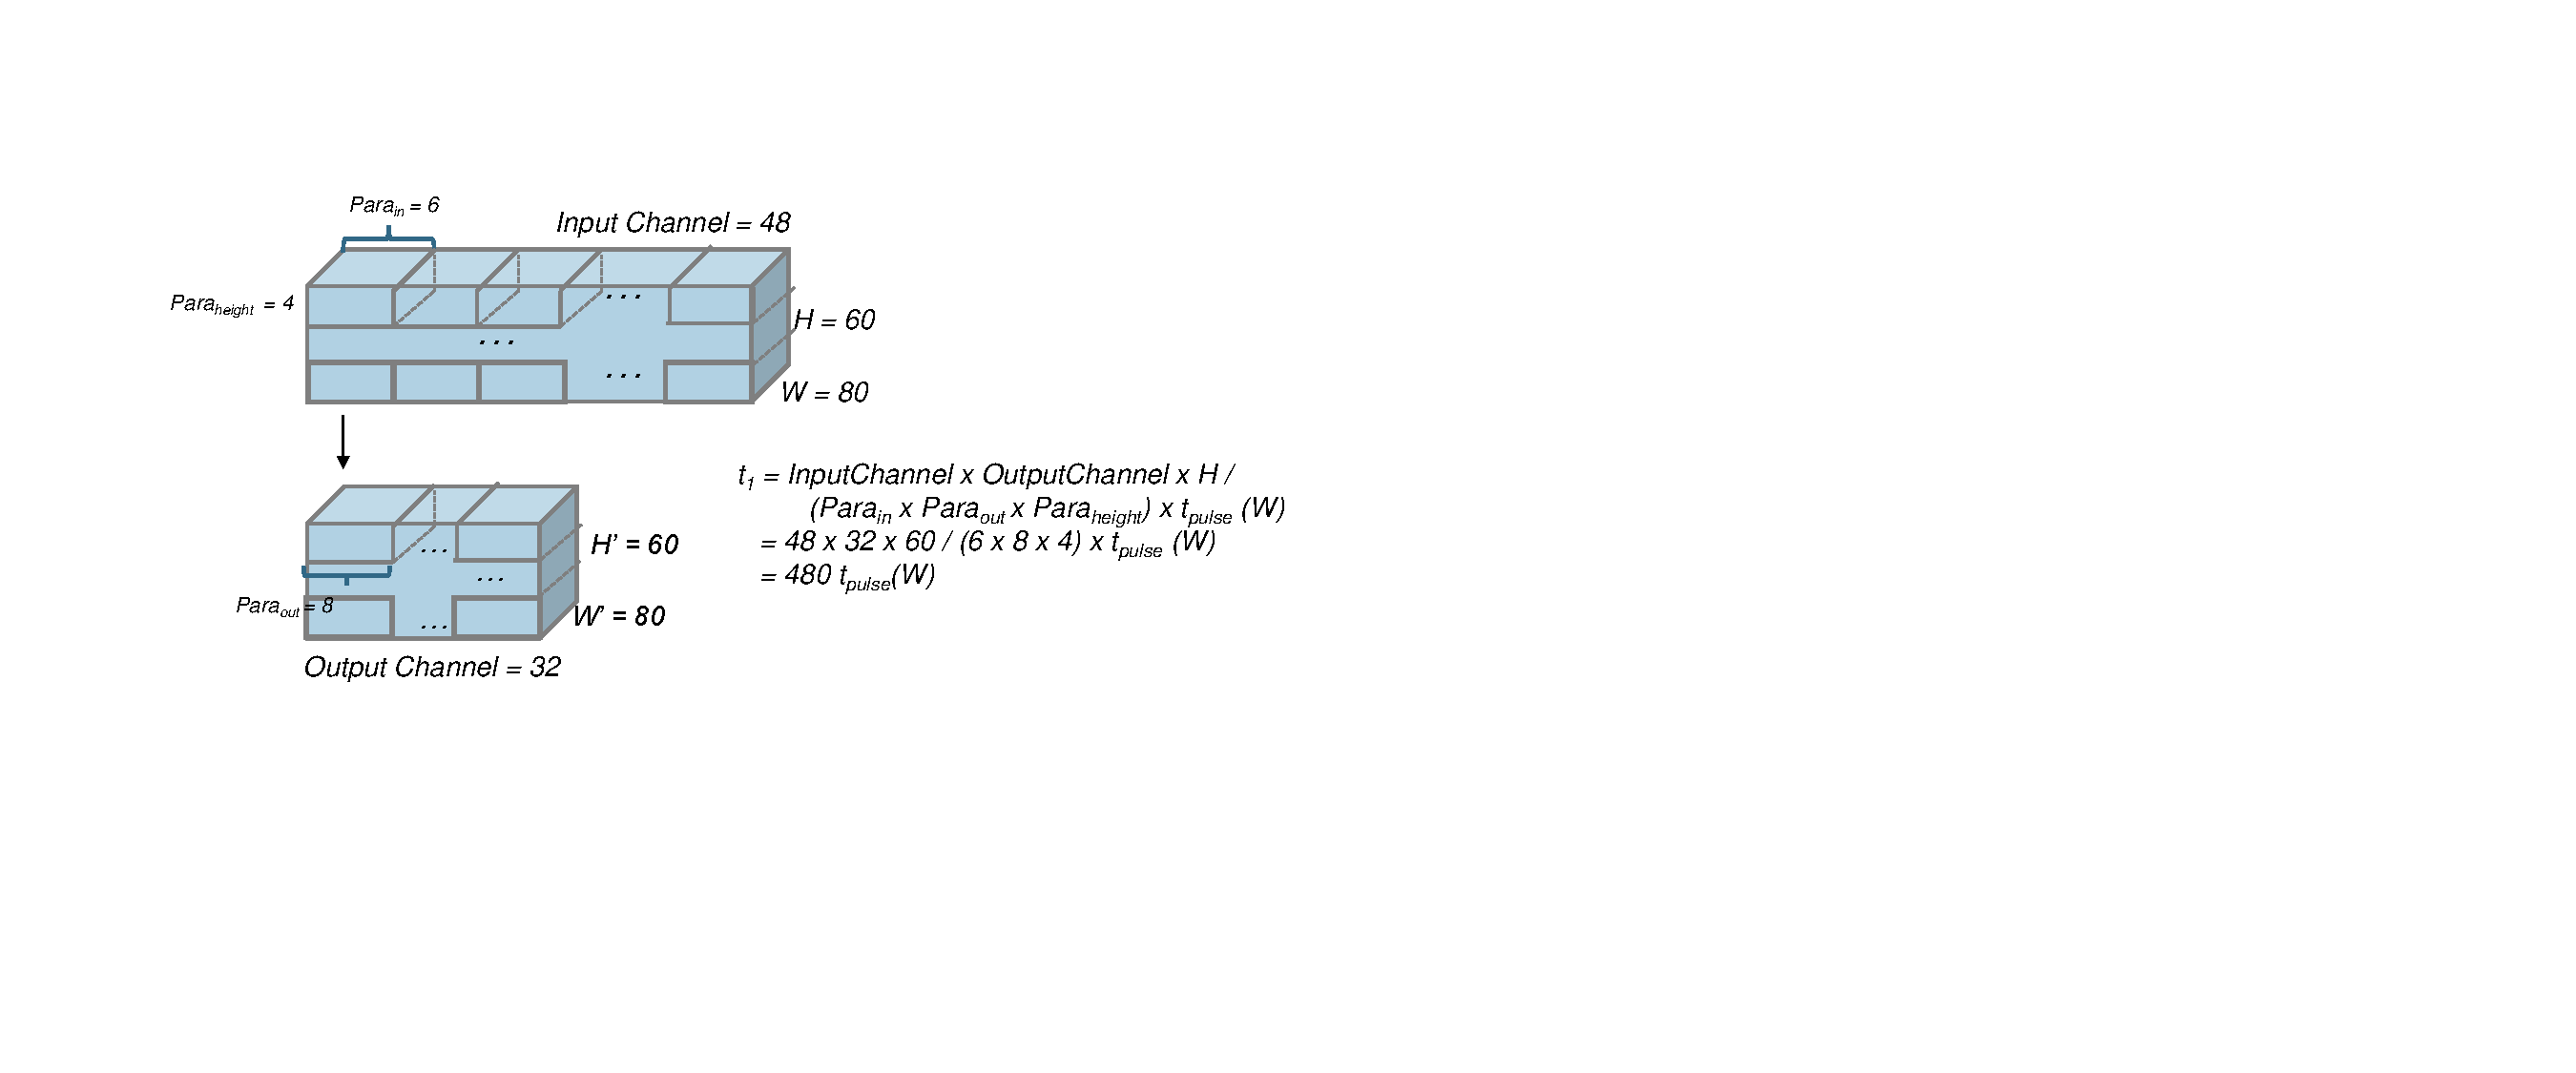
\includegraphics[width=0.99\linewidth]{fig/t1all.pdf}
		\end{minipage}%
	}
	\subfloat[$t_1$ for Virtual-Instruction method]{
		\begin{minipage}[t]{0.45\linewidth}
			\centering
	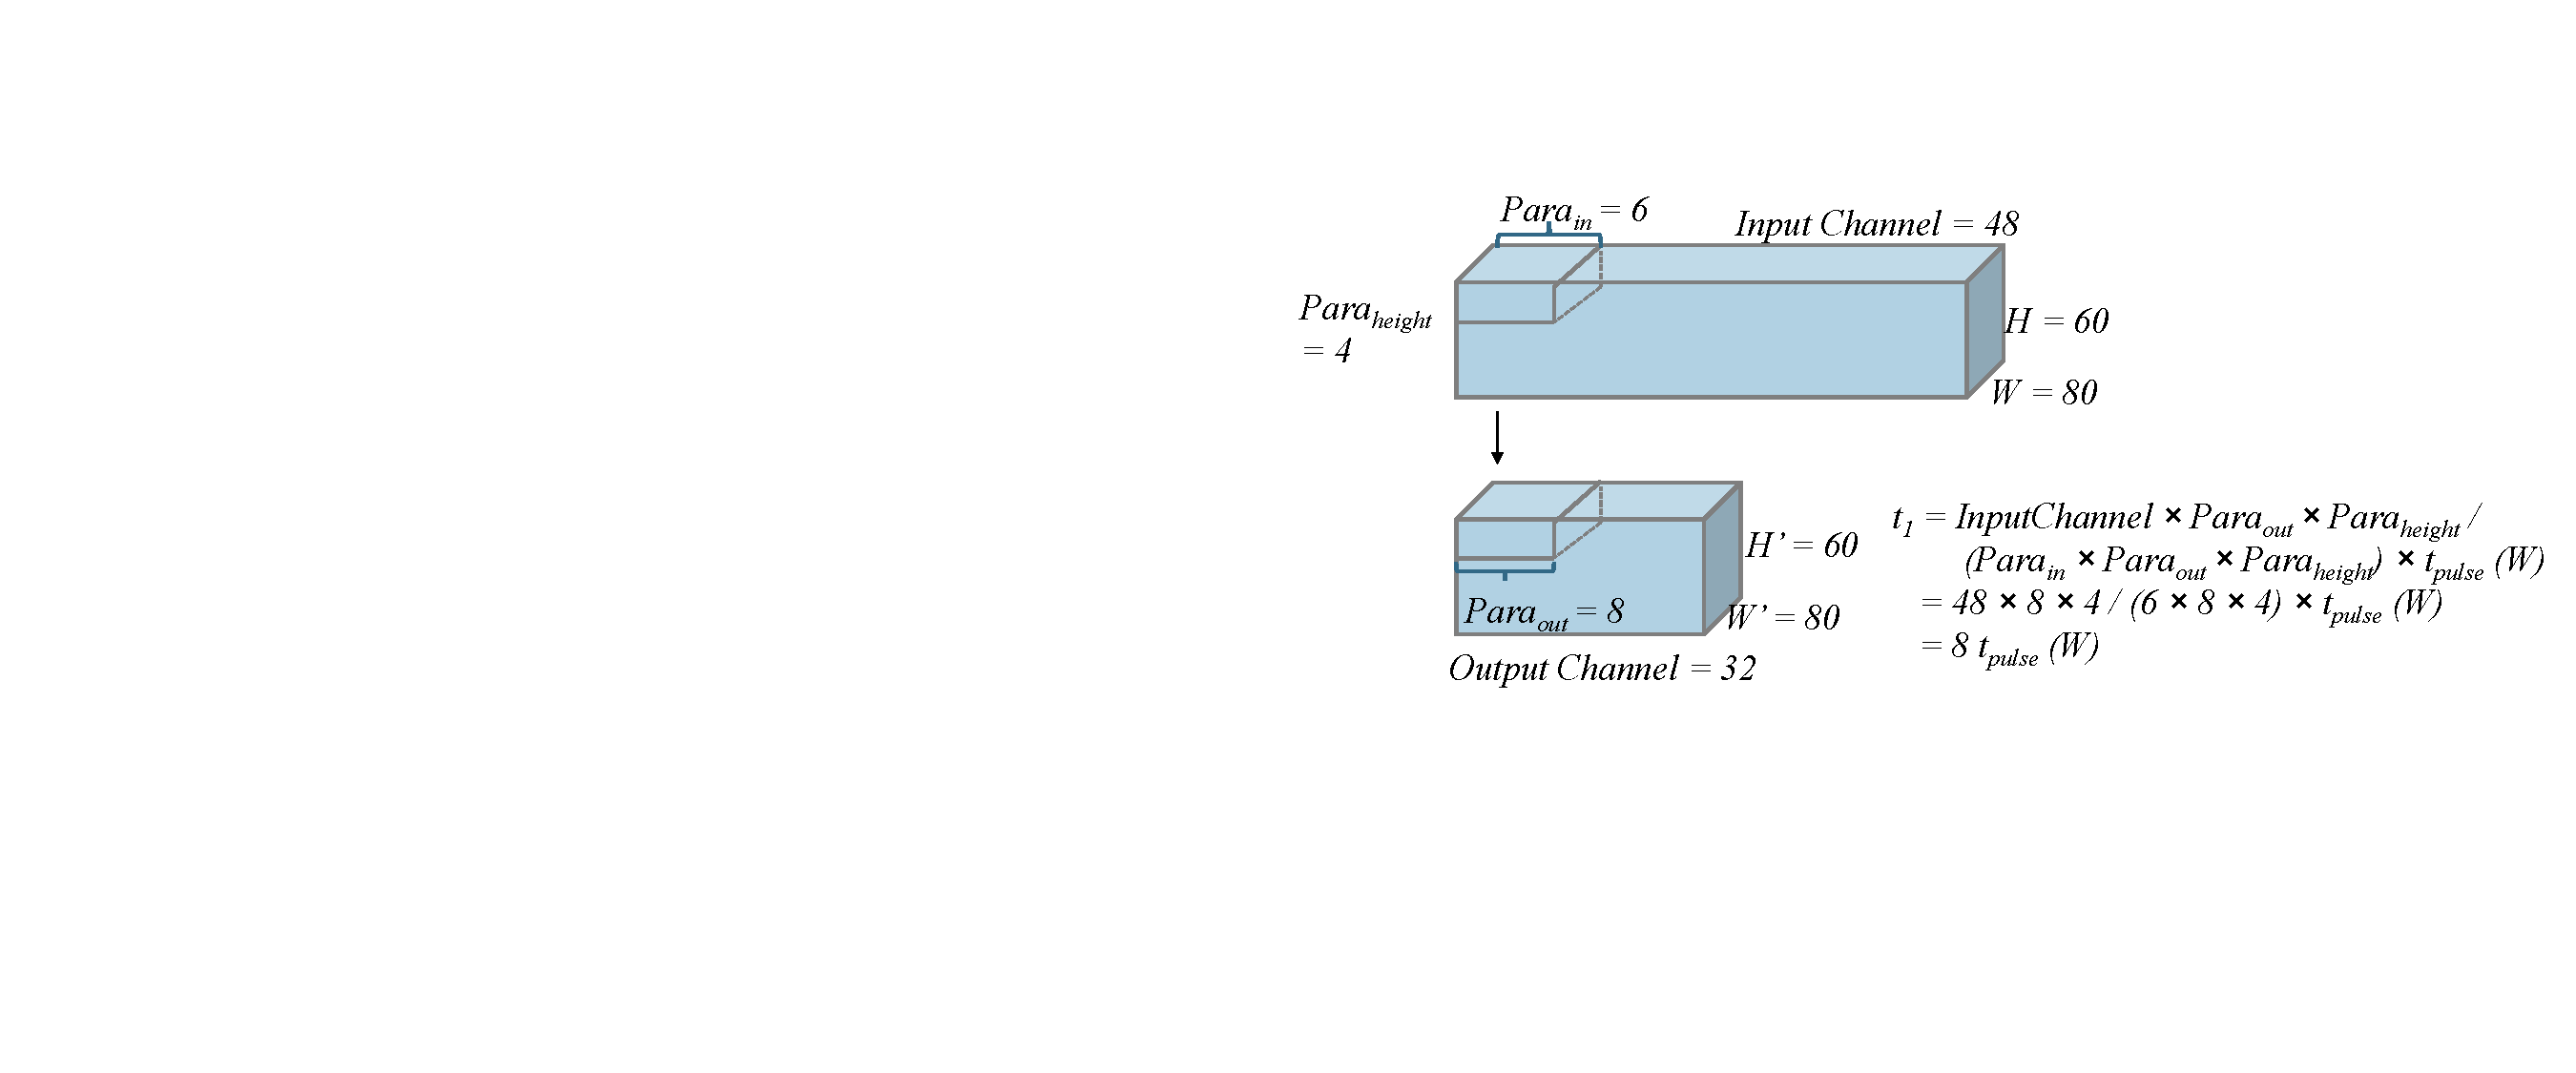
\includegraphics[width=0.99\linewidth]{fig/t1after.pdf}
		\end{minipage}%
	}
	\vspace{-1mm} 
	\caption{ An example of waiting time for finishing the current operation ($t_1$) in a convolution layer. Compared with the Layer-By-Layer method, the waiting time of our Virtual-Instruction method is reduced to $1.6\%$ in this example. The reduction in latency is related to the height ($H$) of the input featuremaps.  }
	\label{fig:t1example}
\end{figure*}



\subsection {Latency Analysis}

In this subsection, we quantitatively analyze the impact of interruptible position on interrupt respond latency. 
As introduced in \Cref{sec:instrAcc}, each CALC  instruction processes the convolution according to the hardware parallelism with $Para_{height}$ lines from $ Para_{in} $ input channels to $ Para_{out}$ output channels. 
We here note the computation of a CALC instruction an $instruction pulse$, or $pulse$.
The compuatation time of each pulse is related to the hardware architecture and the width of the convolution layer. The larger the width, the larger the workload of a single calculation instruction, and thus the CALC instruction consumes more time. We note the time consumption of a pulse as a function of the featuremap width, $t_{pulse}$:

\begin{equation}
	t_{pulse}(W) = t_{Calc\_Hardware} \times W
\end{equation}

$t_{Calc\_Hardware}$ indicates the time for hardware to produce the intermediate results of one pixel, which is defined by the hardware design and the clock frequency. $W$ is the width of the featuremaps, indicating the workload of the instruction.

\Cref{fig:t1example}(a) shows the worst case of waiting for finishing the current operation of the Layer-By-Layer interrupt method. The worst case is that the interrupt request occurs at the beginning of the layer. In this case, the accelerator will wait until finishing the whole layer. The calculation of the whole layer consists of $N_{pulse\_layer}$ successive CALC instructions. We note the worst time of waiting to finish the current layer, which is the total time of these pulses, as $t_{1\_layer}$.

\begin{equation}
	\small
	N_{pulse\_layer} = \frac{ Ch_{in} \times Ch_{out} \times H }{ (Para_{in} \times Para_{out} \times Para_{height}) } 
\end{equation}

\begin{equation}
t_{1\_layer} = N_{pulse} \times t_{pulse}(W)
\end{equation}

$Ch_{in}$ and $Ch_{out}$ is the number of input channels and output channels. $H$ is the height of featuremaps.

On the other hand, if the execution of the CNN accelerator can be interrupted after SAVE/CALC\_F instructions, the worst case of waiting for finishing the current operation is illustrated in \Cref{fig:t1example}(b). The calculation of the whole CalcBlob consists of $N_{pulse\_VI}$ successive CALC instructions. We note the worst waiting time in this case as $t_{1\_VI}$.

\begin{equation}
	\small
	N_{pulse\_VI} = \frac{ Ch_{in} \times Para_{out} \times Para_{height} }{ (Para_{in} \times Para_{out} \times Para_{height}) } 
\end{equation}

\begin{equation}
t_{1\_VI} = N_{pulse\_VI} \times t_{pulse}(W)
\end{equation}


Because our Virtual-Instruction method (VI method) only interrupts the execution after CALC\_F and SAVE, there is no extra data transfer for the intermediate results. The backup operation in the VI method only transfers the final results, which are also transfered to DDR with the SAVE instructions in the Layer-By-Layer method. Experiment results in, which will be given in \Cref{sec:expt1t2}, show that the data transfer time for the final results is much less than the calculation time (less than 20\%), in both the Layer-By-Layer method and the VI method. Thus the latency to respond to the interrupt request ($t_{latency}$) is mainly determined by the time of finishing the current operation.

As the interrupt request is unpredictable, we model the interrupt location as evenly distributed within each layer. Thus the average interrupt latency is $\bar{t}_{latency} $.

\begin{equation}
	\bar{t}_{latency}  \simeq \frac{1}{2} \times t_{1}
\end{equation}

Compared with the Layer-By-Layer method, the latency of our method is reduced to $R_l$.

\begin{equation}
	\small
	\begin{split}
	R_l & =  \frac{\bar{t}_{latency\_VI}}{\bar{t}_{latency\_layer}} \simeq \frac{\frac{1}{2} \times t_{1\_VI}}{\frac{1}{2} \times t_{1\_layer}}  = \frac{ N_{pulse\_VI} \times t_{pulse}(W) }{ N_{pulse} \times t_{pulse}(W) }  \\
		   & = \frac{ N_{pulse\_VI} }{N_{pulse} } = \frac{ Ch_{in} \times Para_{out} \times Para_{height}  }{  Ch_{in} \times Ch_{out} \times H } \\
		   & = \frac{ Para_{out} \times Para_{height} }{ Ch_{out} \times H} 
	\end{split}
\end{equation}

$\bar{t}_{latency\_VI}$ and $\bar{t}_{latency\_VI}$ are the average interrupt latency of the Virtual-Instruction method and the Layer-By-Layer method. The effect of latency reduction of the VI method is related to the number of output channels ($Ch_{out}$) and featuremap height ($H$). The larger the featuremaps output channels and the height, the better latency reduction result can be achieved.

An example of a convolution layer with a typical size in CNN is given in \Cref{fig:t1example}. The parameters are labelled in the figures. The latency can be reduced to $R_t = 8/480 =1.6\%$.



\subsection{Virtual Instruction ISA (VI-ISA) }
\label{sec:virtualinstr}

We add two fields to the instruction set: 1) Virtual and 2) SaveID, as illustrated in \Cref{fig:instructions}(b). 

\textbf{   Virtual Field}. The virtual instructions should be only valid when interrupt occurs. So we add a field in the original ISA, that indicates whether the instruction is a virtual instruction. If no interrupt occurs, virtual instructions will be skipped and discarded, which can ensure the efficiency of uninterrupted execution. Three values can be set to Virtual Field:
% \begin{itemize}

	\textit{2'b00} indicates this instruction is not virtual, should always be executed.
	
	\textit{2'b01} indicates this instruction is the SAVE instruction for backup. When an interrupt occurs, the high-priority network will start after this instruction.
	
	\textit{2'b10} indicates this instruction is the LOAD instruction for recovery. The corresponding instructions will be executed after the high-priority network.
% \end{itemize}

\textbf{ SaveID Field }
SaveID links CalcBlob instructions to the corresponding SAVE. SaveID of each not-virtual SAVE instruction differs. If the generated outputs of CalcBlobs are stored to DDR by a SAVE instruction, the CalcBlobs have the same SaveID as the SAVE instruction.

% The SaveID for a CalcBlob is the same as its CALC\_F instruction.
One SAVE instruction can correspond to one CalcBlob (Single Blob Save, illustrated in \Cref{fig:singlesave}(b)) or multiple CalcBlobs (Multiple Blob Save, illustrated in \Cref{fig:singlesave}(c)).

For Single Blob Save, no virtual SAVE is added. The high-priority network can be started after the original not-virtual SAVE. The virtual LOAD instructions for data recovery are generated after the original SAVE, and executed after the high-priority network. The execution timeline is shown in \Cref{fig:singlesave}(d).

For Multiple Blob Save, virtual SAVE and LOAD instructions are generated after the CALC\_F of each CalcBlob. When the interrupt request occurs, the virtual SAVE instruction will be executed before the start of the high-priority network. Virtual LOAD instructions for data recovery are executed after the high-priority network. The subsequent original not-virtual SAVE instruction with the same SaveID as the CalcBlob will be modified to avoid duplicate output data transfer. The execution timeline is shown in \Cref{fig:singlesave}(e).


\begin{figure}[t]
	\centering
    % \vspace{-0.1cm} 
    % \setlength{\abovecaptionskip}{0cm} 
    % \setlength{\belowcaptionskip}{-0.4cm} 
	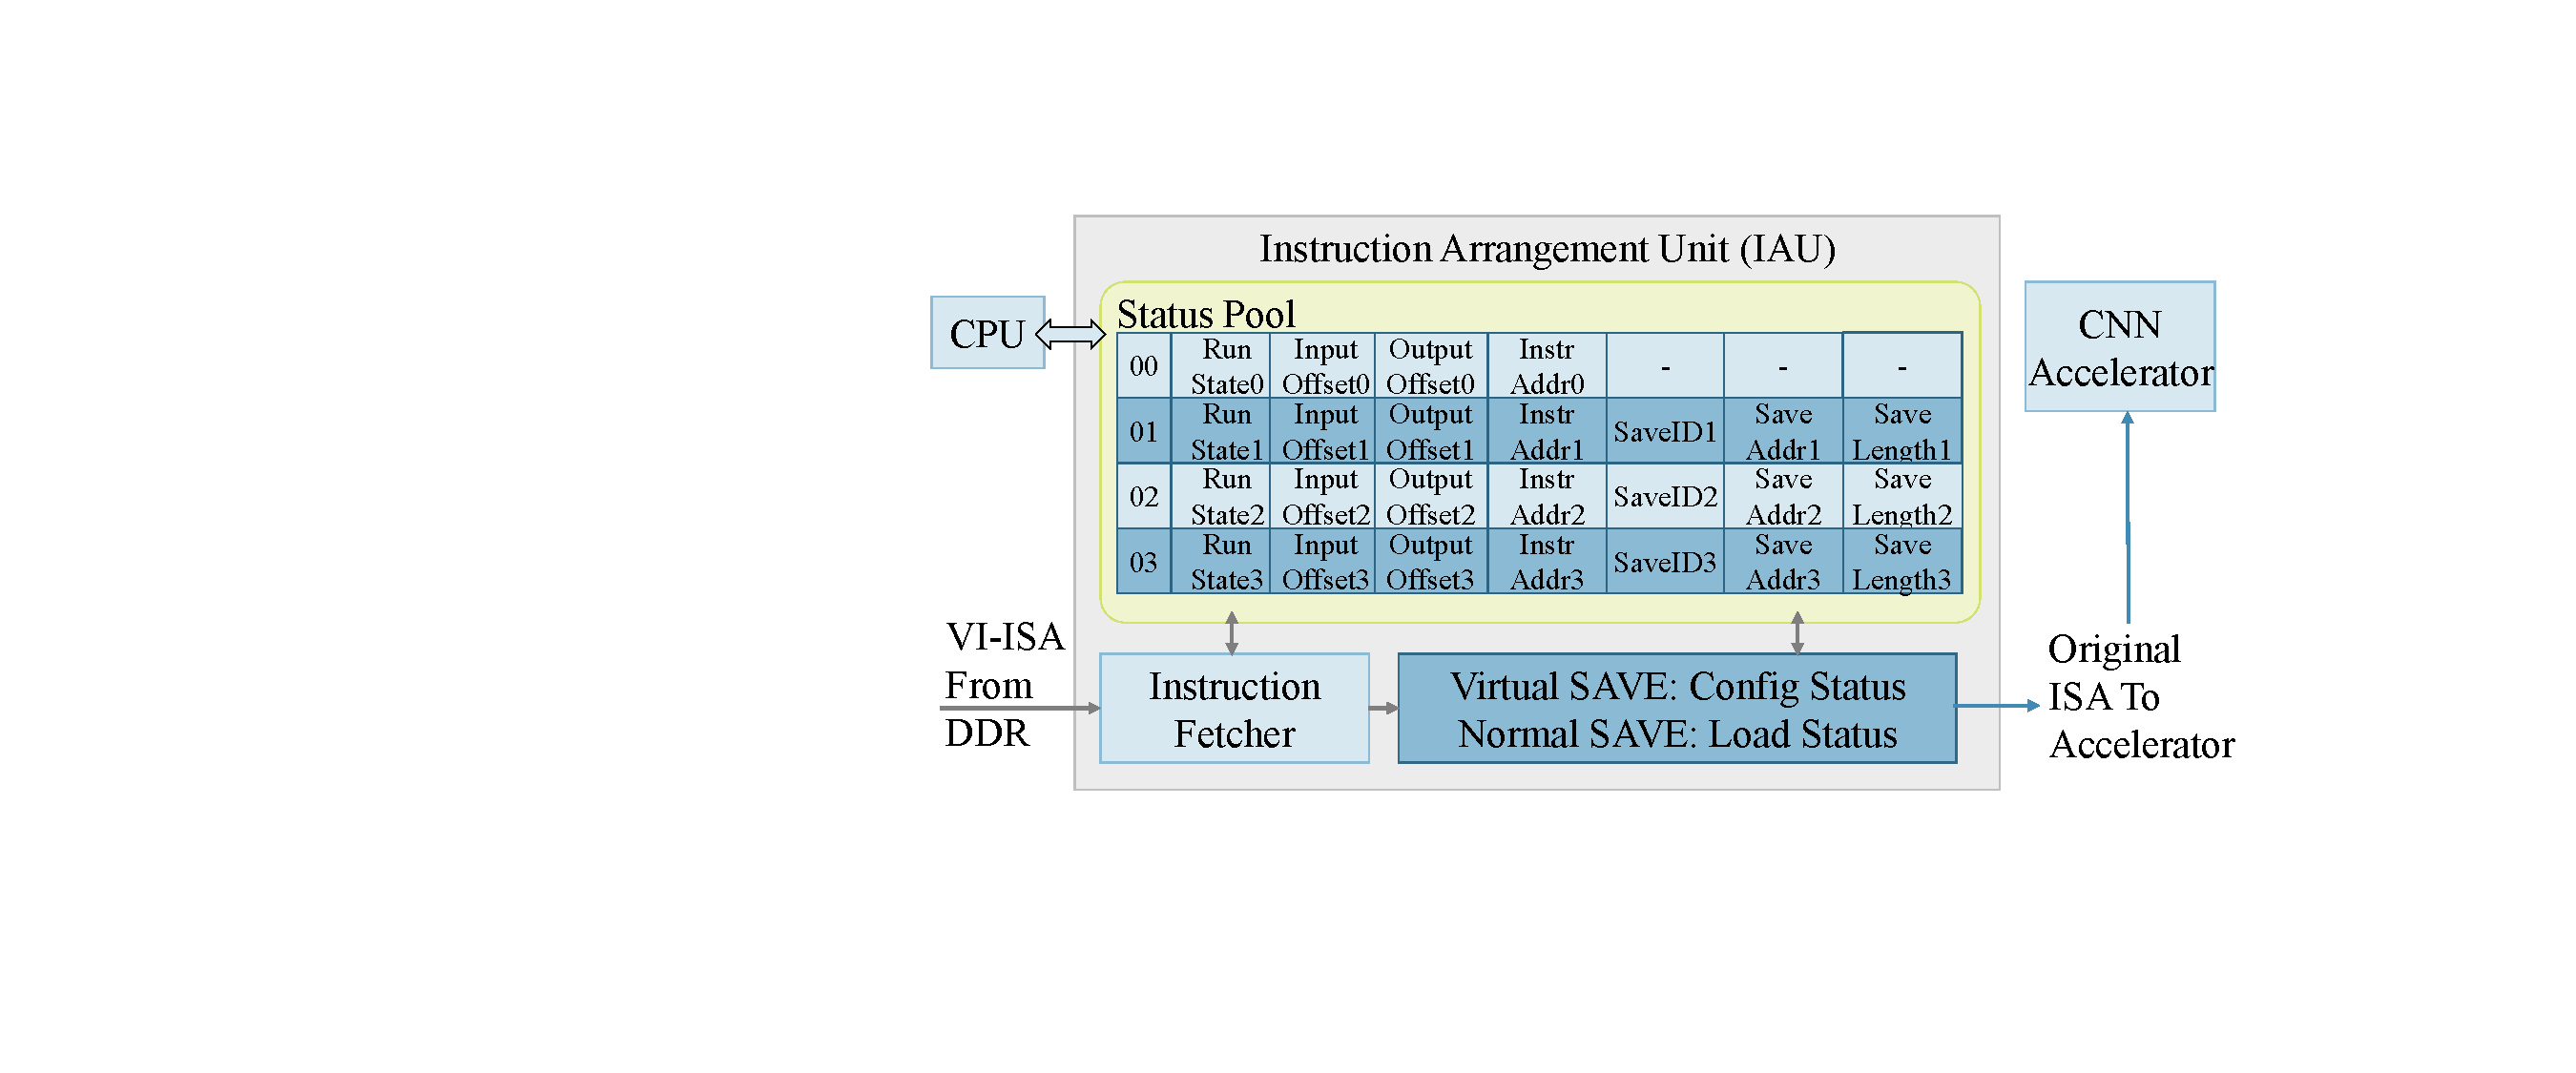
\includegraphics[width=0.99\linewidth]{fig/iau.pdf}
	\vspace{-6mm}
	\caption{Hardware architecture of IAU. The software on the CPU (PS side) communicates with IAU to access the CNN accelerator. IAU records the running state of each task and translates the input instruction virtual instructions sequence (VI-ISA) to a normal sequence of instructions (Original ISA).
	}
	\label{fig:IAU}
\end{figure}
\begin{figure*}[t]
	\centering
    % \vspace{-0.1cm} 
    % \setlength{\abovecaptionskip}{0cm} 
    % \setlength{\belowcaptionskip}{-0.05cm} 
	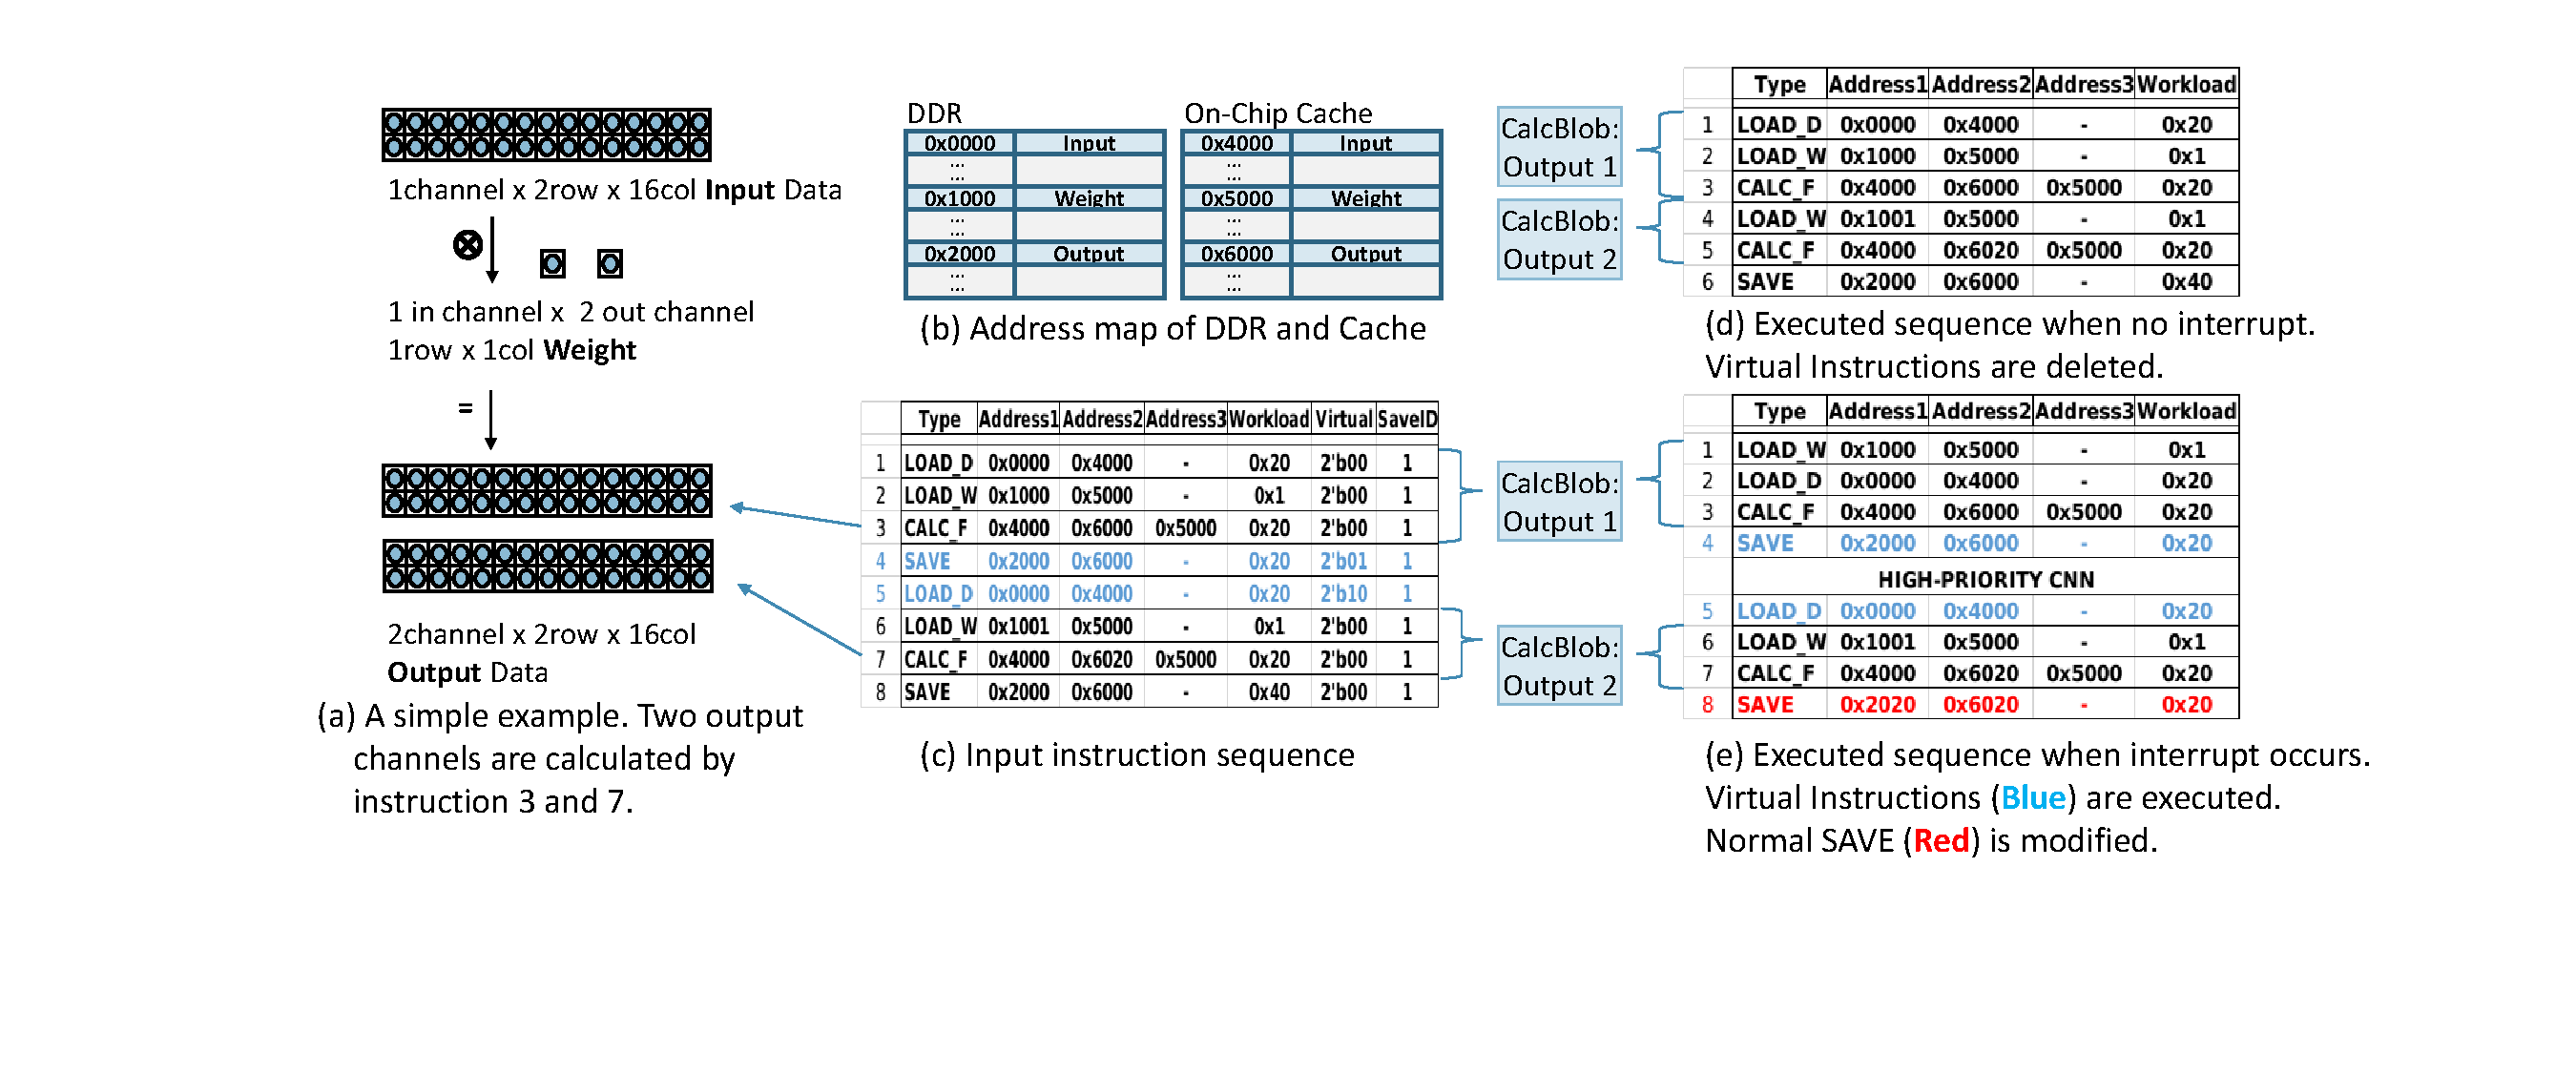
\includegraphics[width=0.9\linewidth]{fig/interexample.pdf}
	\vspace{-5mm}
	\caption{ A simple example of our proposed virtual-instruction-based interrupt. Fig(a), the CNN layer structure. Fig(b), the on-chip and DDR addresses of different data. Fig(c), the instruction sequence in virtual instruction ISA (VI-ISA). The blue instructions are the virtual SAVE and LOAD. Fig(d), executed instructions when no interrupt occurs. Fig(e), executed instructions when an interrupt occurs. }
	\label{fig:interexample}
\end{figure*}


\subsection{ Instruction Arrangement Unit (IAU) }

Instruction Arrangement Unit (IAU) is the hardware to handle the computing requirements of different priority tasks. The IAU monitors the interrupt status and generates the original ISA instruction sequence. The original CNN accelerator does not need to know the interrupt status, and only operates the instructions provided by IAU.

The hardware implementation of IAU is shown in \Cref{fig:IAU}, which supports four tasks with different priorities. Task 0 has the highest priority and is not interruptible. 
InstrAddr records the address to fetch the instructions of the corresponding task. The InputOffset and the OutputOffset, which indicate base address offsets of the input and output data, are configured by the software. 
SaveID, SaveAddr, and SaveLength record the status when an interrupt occurs. 
Subsequent not-virtual SAVE instructions will be modified according to the recorded interrupt status (SaveID, SaveAddr, and SaveLength), to avoid duplicate output data transfer.
% An example of the instruction modification will be given at \Cref{sec:exampleVirtual}.


\subsection{Example of Virtual Instruction}
\label{sec:exampleVirtual}


The example is based on a straightforward convolutional layer, which has only one input channel and two output channels. 
The convolution kernel size is $1 \times 1$. The shape of the input and output featuremaps is $ 2 \times 16 $ (\Cref{fig:interexample}(a)). The parallelism of the CALC instruction in this example is $ Para_{in} = 1$ , $ Para_{out}=1$ , $Para_{height}=2$.

Thus, the two output channels are calculated by two CALC\_F instructions (instruction 3 and 7 in \Cref{fig:interexample}(c)). The addresses used in the instruction example are listed in \Cref{fig:interexample}(b). \Cref{fig:interexample}(c) is the instruction sequence from DDR with VI-ISA. \Cref{fig:interexample}(d) is the executed original ISA instructions without interrupt. When an interrupt occurs at the first CalcBlob, \Cref{fig:interexample}(e) illustrates the backup/recovery instructions (Blue) and the modified SAVE instruction (Red). 
% IAU monitors the interrupt status and translates the VI-ISA instruction sequence to the original ISA instruction sequence.

% The hardware implementation of IAU is shouwn in \Cref{{fig:IAU}. There is a Status Pool which records the running states of each task. The InstrAddr is records the instruction address of each CNN

\section{Optimization For Post-Processing }
\label{sec:hardsoftcodesign}
\label{subsec:FEopt}

The high-priority feature-point extraction (FE) task is latency-sensitive and needs to be computed before the next input frame arrives. With the help of the CNN accelerator, the latency of CNN backbone is reduced. However, the post-processing of FE on the embedded CPU consumes more than 50ms, which becomes the bottleneck of the real-time system. In this section, the software and hardware acceleration for CNN-based FE method is introduced.


The flow path of our SuperPoint-based feature extraction method is shown in \Cref{fig:superpoint}. 
The SuperPoint backbone maps the input image $I\in \mathbb{R}^{H\times W}$ to a tensor $\mathcal{X}\in \mathbb{R}^{H_c\times W_c\times 65}$ for feature-point detection and to a tensor $\mathcal{D}\in \mathbb{R}^{H_c\times W_c\times D}$ for descriptors generation, where $H_c = H/8$ and $W_c = W/8$.
We optimize the software data flow of the components above, making them less computationally complex and more friendly to hardware. 

% As mentioned in \Cref{sec:relate}, there are two steps in the FE method: 1) feature-point detection and 2) feature descriptors generation. 
In SuperPoint~\cite{detone2018superpoint}, there are three components in the feature-point detector: 1) Softmax to generate confidence for each pixel. 2) Non-Maximum Suppression (NMS) to find the pixels with maximum confidence in its neighborhood. 3) Rank component to find out the first $k$ pixels with the highest confidence. 
In the feature descriptor generator, the normalization component consumes most of the computation. 
Then we design specifical FPGA accelerators for softmax and normalization.

\subsection{Optimization of Feature-point Detection}
\label{sec:softmaxopt}

\begin{figure}[t]
 \centering 
 % \vspace{-0.1cm} 
 % \setlength{\abovecaptionskip}{0cm} 
 % \setlength{\belowcaptionskip}{-0.05cm} 
 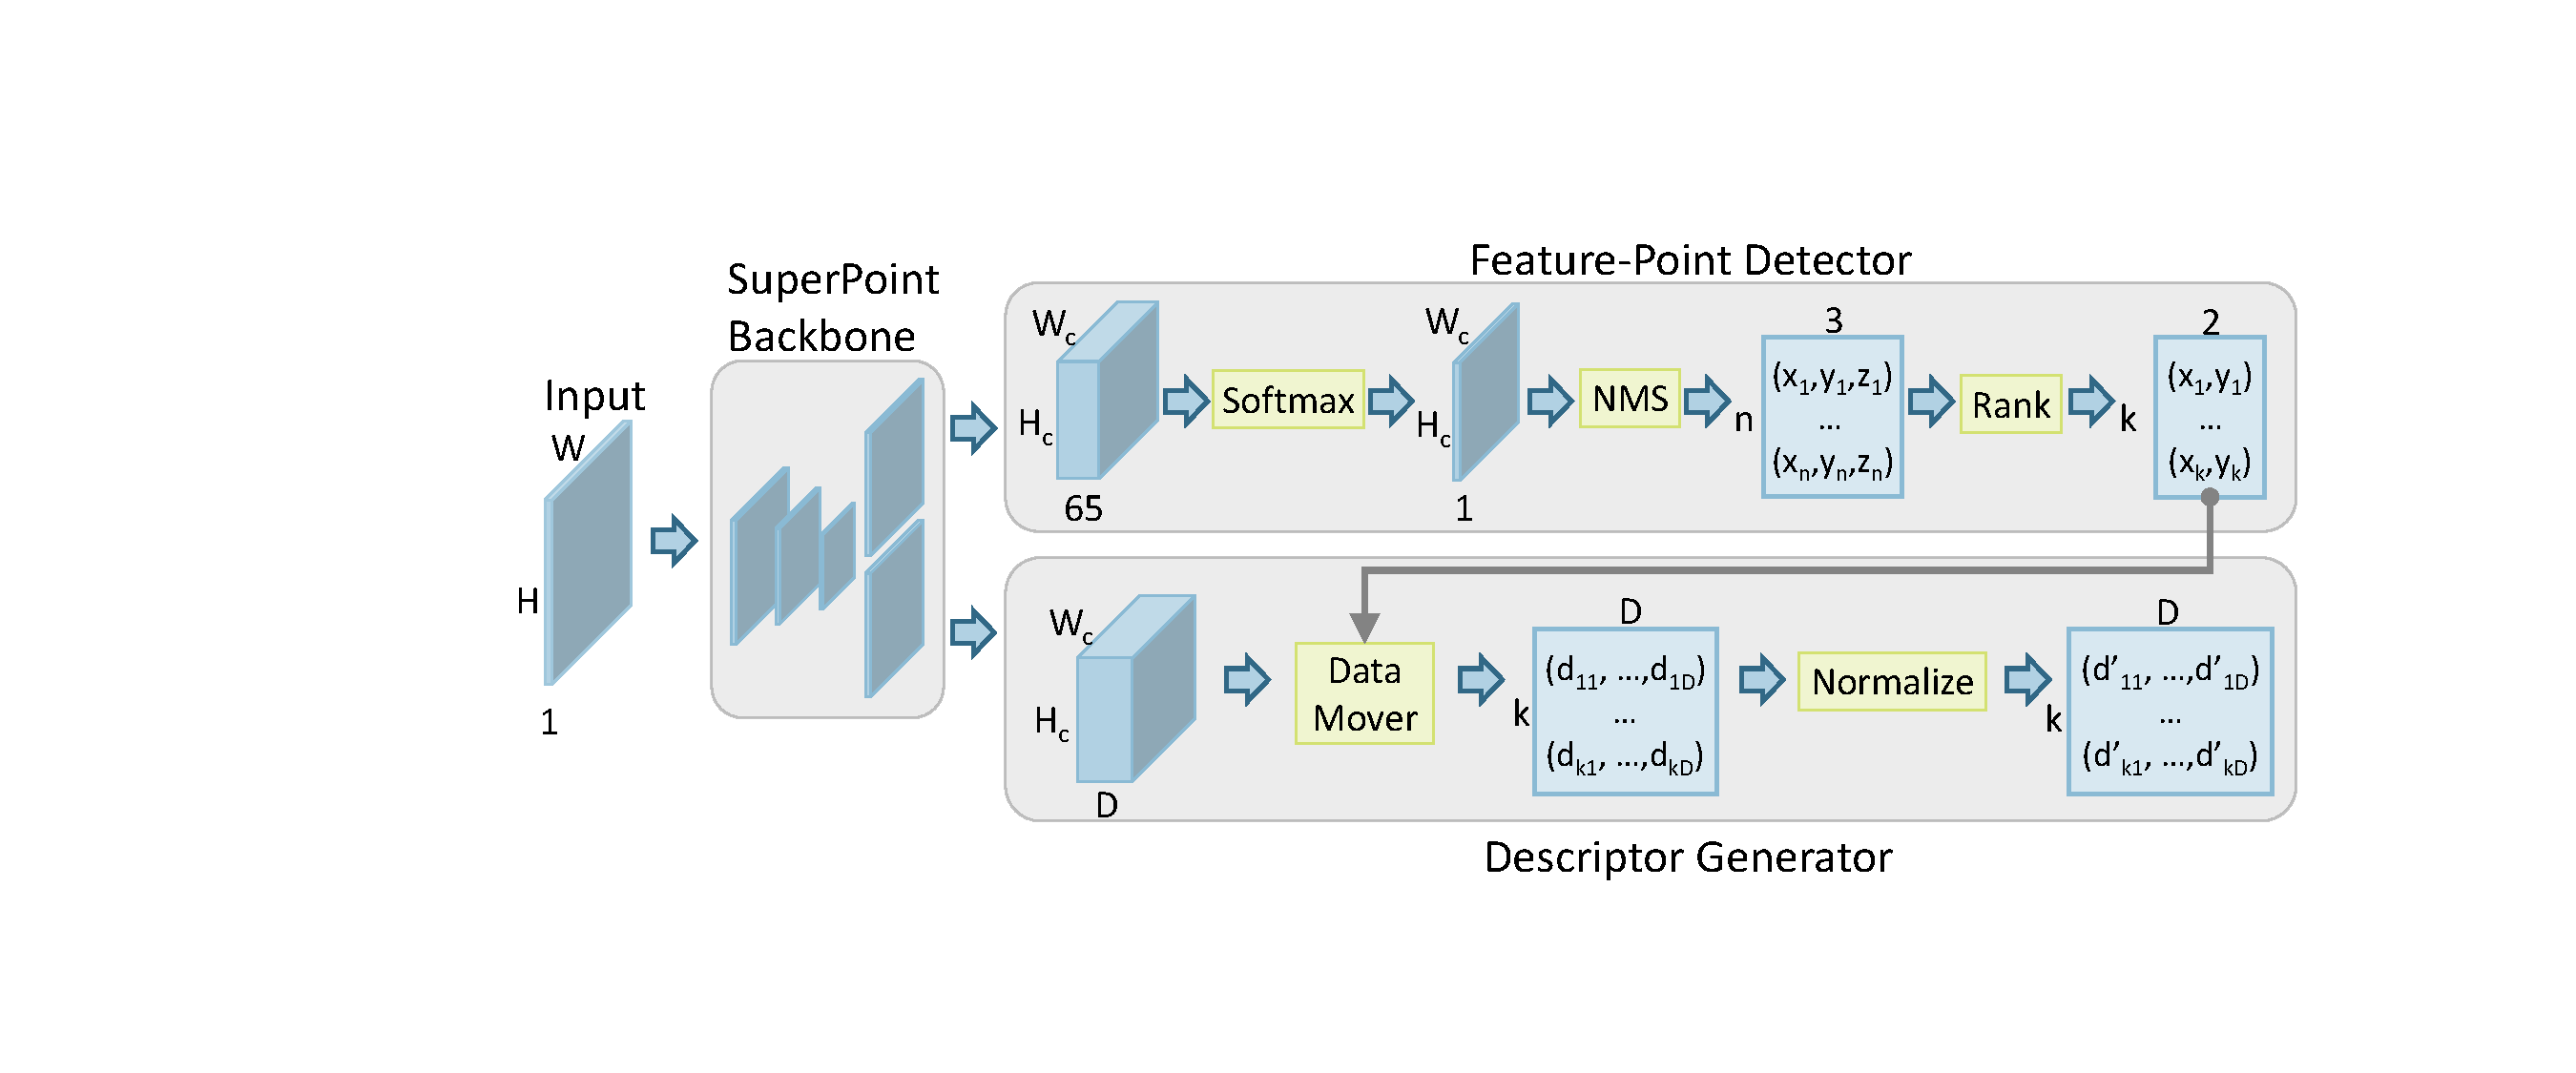
\includegraphics[width=0.99\linewidth]{fig/superpoint.pdf}
 \vspace{-8mm}
 \caption{Optimized feature-point extraction method based on SuperPoint. Instead of calculating the normalized descriptors for all pixels, we only need to calculate the normalized descriptors for the pixels with the highest confidence after ranking.}
 \label{fig:superpoint}
\end{figure}

\begin{figure}[t]
 \centering 
 % \vspace{-0.1cm} 
 % \setlength{\abovecaptionskip}{0cm} 
 % \setlength{\belowcaptionskip}{-0.2cm} 
 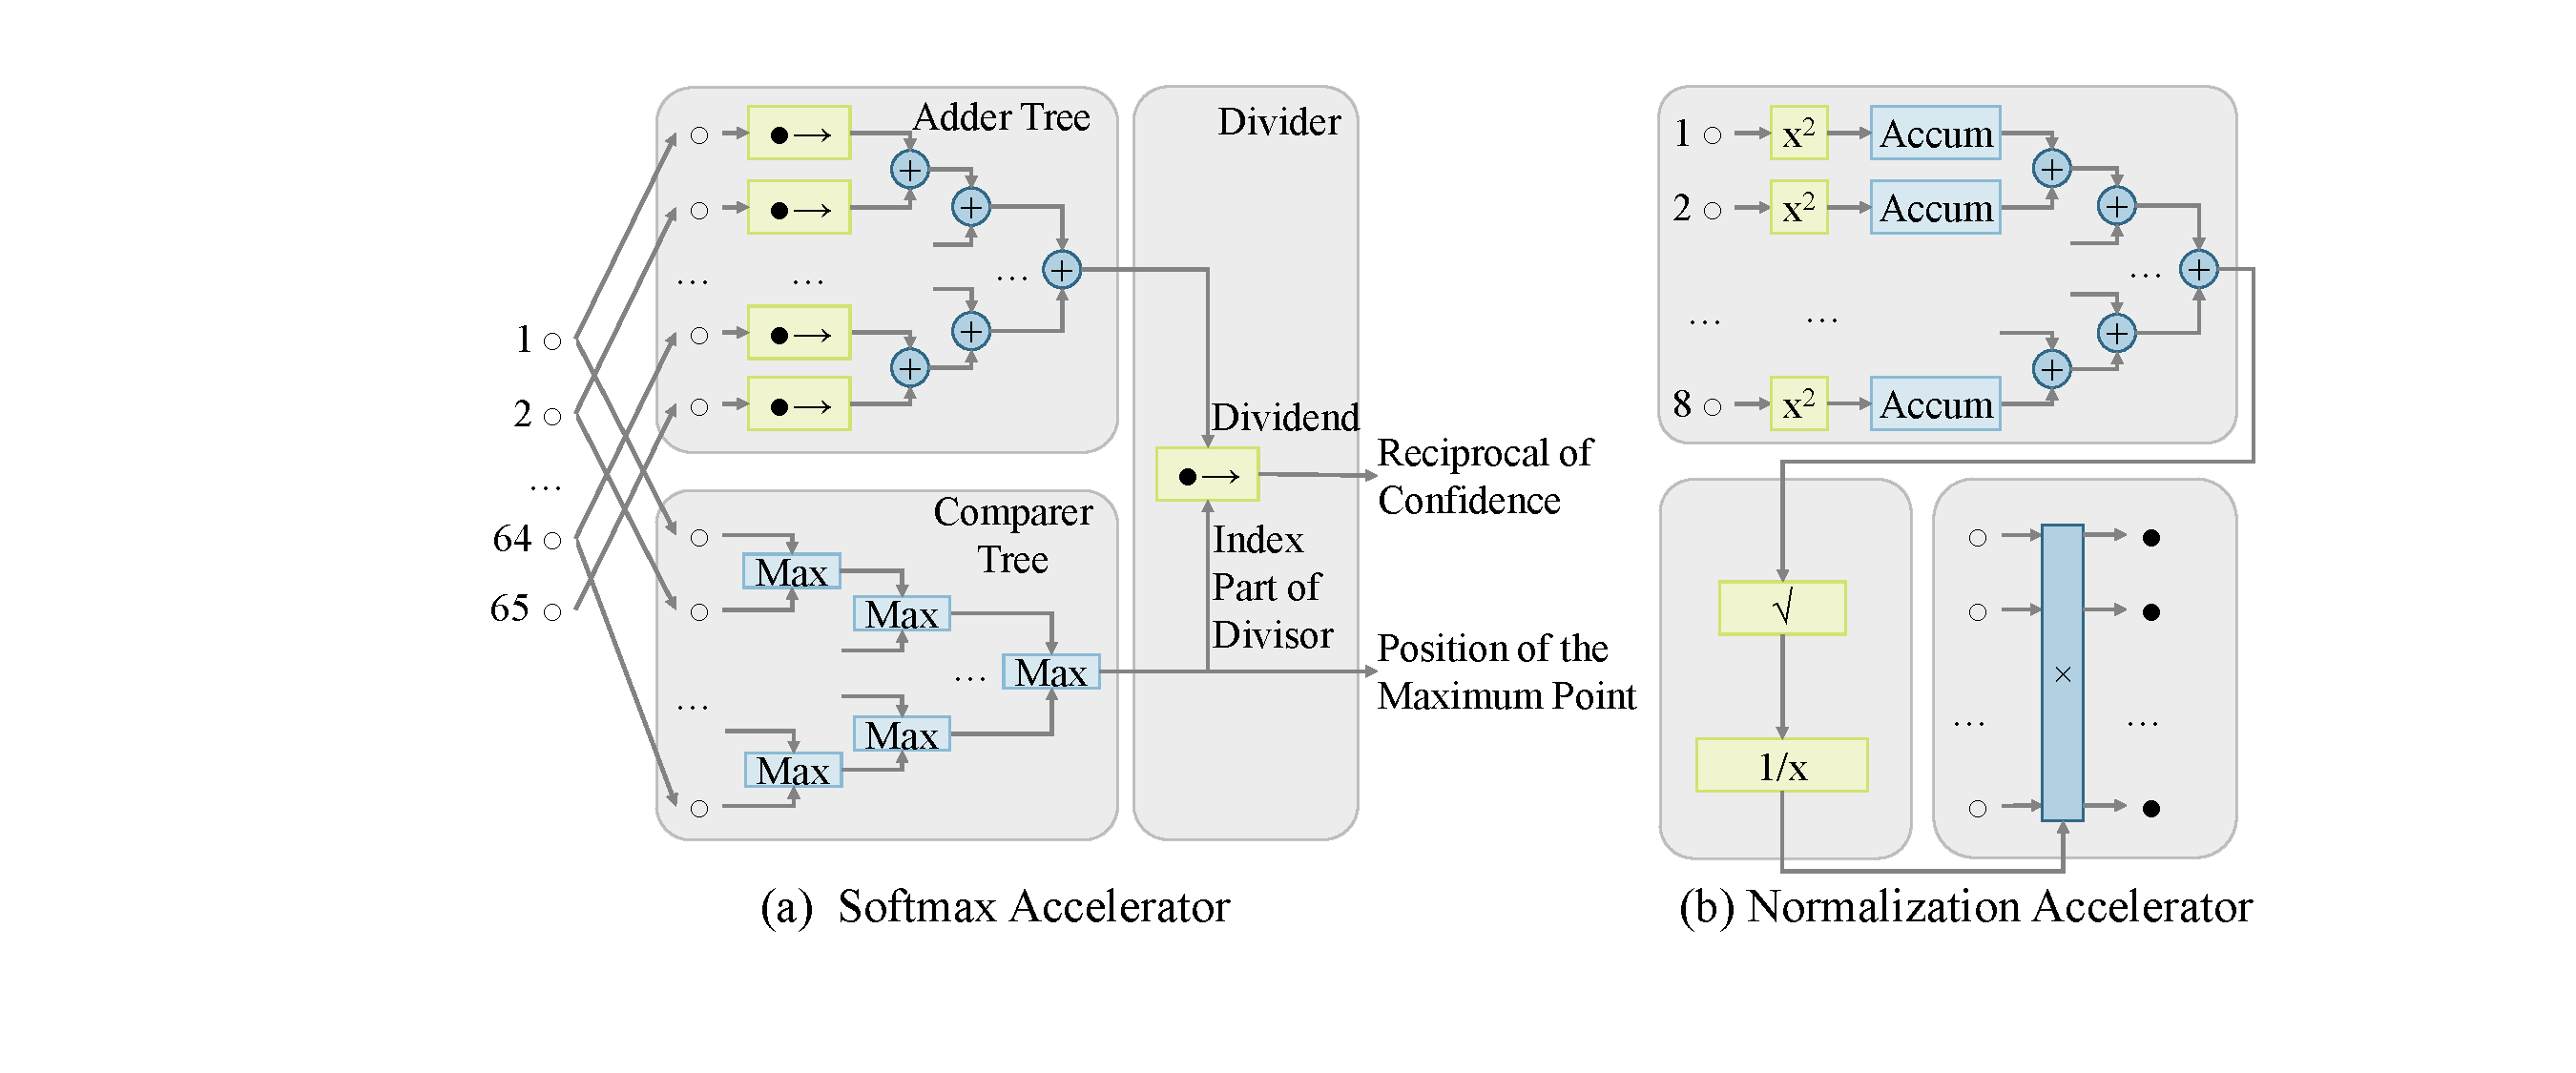
\includegraphics[width=0.99\linewidth]{fig/FEaccelerator.pdf}
 \vspace{-7mm}
 \caption{Hardware Architecture of FE Accelerators. Fig(a), we design an adder tree together with a comparer tree, so that only the softmax value of the element with the highest confidence is calculated instead of calculating all the 65 softmax values. Fig(b), the adder tree process the partial square sum of 8 input elements once, and we use 32 clocks to finish the square sum of all the 256 elements.}
 \label{fig:FEaccelerator}
\end{figure}

For feature-point detection, the 65 channels correspond to local, non-overlapping $8 \times 8$ pixel grid areas plus a background channel. 
After a channel-wise softmax, the background channel is removed, and a $\mathbb{R}^{H_c\times W_c\times64}\Rightarrow \mathbb{R}^{H\times W}$ reshaping is performed. 
% The channel-wise softmax makes the points in different grid areas have equal confidences.
The tensor of size $\mathbb{R}^{H\times W}$ corresponds to the confidences of the feature points in the input image. The higher the confidence, the more likely this point is to be a feature-point.

The standard softmax function is defined as $\sigma (\mathbf {z} )_{i}$ in \Cref{equ:softmax_hard}.
We optimize the process of softmax that we only take the maximum value of each grid area for subsequent computations, which not only reduces the division operations of softmax but also simplifies the calculation of NMS and Rank.
We reduce the division operations and output size of softmax from $H \times W$ to $H_c \times W_c$.
The division operation is resource consuming on the FPGA platform. 
Our method can greatly reduce the number of divisions by $64 \times$, making it easy to accelerate softmax operation on FPGA.

\begin{equation}
 \small
 \sigma (\mathbf {z} )_{i}={\frac {e^{z_{i}}}{\sum _{j=1}^{K}e^{z_{j}}}}
 \Rightarrow
 \frac{1}{\sigma (\mathbf {z} )_{i}}={\frac {\sum _{j=1}^{K}2^{z_{j}}}{2^{z_{i}}}}{\text{ for }}i=1,\dotsc ,64;
 \label{equ:softmax_hard}
\end{equation}

Since the results of the softmax function are all positive, we can calculate the reciprocal of the softmax function ($\frac{1}{\sigma (\mathbf {z} )_{i}}$) in \Cref{equ:softmax_hard} as the normalized confidence, without affecting the results of the NMS and ranking process. We quantize the output feature map of CNN to 8-bit fixed-point number, i.e each $z_i$ in \Cref{equ:softmax_hard} is a 8-bit fixed-point number. We change the base of the power from $e$ to $2$ to make it more hardware friendly. Since the divisor is a power of $2$, we can also implement division by shift operation.

\Cref{fig:FEaccelerator}(a) shows an overview of the softmax module. It consists of three parts: adder tree, comparer tree and divider. Softmax reads 65 numbers from a grid region at once. Adder tree computes input to the power of $2$ using shift operation and calculates their sum. Comparer tree reads the values of the first 64 channels and returns the maximum value, as well as its channel number which contains the position information. The divider uses the shift operation to calculate the reciprocal of confidence.

NMS is applied to the detection to ensure that the feature-points are evenly distributed throughout the image. 
For each pixel in the original input image, NMS compares the confidence of this pixel with that of the pixels in a square neighborhood whose edge includes $\epsilon _{ori}$ pixels. 
If the confidence of the target central pixel is not the maximum in its neighbors, this point will be eliminated. 
The output of the NMS is a list of coordinates and confidences for each feature-point. 
Since the softmax optimization already gives the pixel with maximum confidence of each $8 \times 8$ block, the total number of pixels is reduced by $64 \times$ and the neighbors of each pixel is reduced by $10 \times$.
The total number of comparisons in NMS is reduced by $640\times$.

The ranking operation is to find out the top $k$ feature-points with maximum confidence after NMS. 
Since we only need to find feature-points without knowing their order, we create a heap of size $k$ to find the $k$ feature-points instead of quick sort~\cite{Niu2012Top}.


% \subsection{NMS Optimization}

% Non-maximum suppression (NMS) is applied to the detection to help ensure that the feature-points are evenly distributed throughout the image. 
% For each pixel in the original input image, NMS compares the confidence of this pixel with that of the pixels in a square neighborhood whose edge including $\epsilon _{ori}$ pixels. 
% If the confidence of the target central pixel is not the maximum in its neighbors, this point will be eliminated from the valid feature-points. 
% The output of the NMS is a list of coordinates and confidences for each feature-point. 
% There are totally $H \times W$ points and the NMS does $\epsilon _{ori} ^ 2 - 1$ comparison operations for each points. 
% Thus, in the original NMS method, there are totally $H \times W \times (\epsilon _{ori} ^ 2 - 1)$ comparison operations.

% The softmax optimization introduced in \Cref{sec:softmaxopt} already gives the pixel with maximum confidence of each $8 \times 8$ block. Thus, we only need to compare each output pixel of softmax to the its adjacent blocks. The comparison area is a square box with an edge of $\epsilon _{opt}$ pixels. and $\epsilon _{opt} = 2\times \left \lceil (\epsilon _{ori}-1)/16 \right \rceil +1$. There are only $H_c \times W_c$ points. Thus, after NMS optimization, there are totally $H_c \times W_c \times (\epsilon _{opt} ^ 2 - 1)$ comparison operations.

% The $\epsilon _{ori}$ is set to 9 in the original implements SuperPoint, so $\epsilon _{opt} = 2\times \left \lceil (\epsilon _{ori}-1)/16 \right \rceil +1 = 3$. So that $H \times W \times 80 $ comparisons are done in the original NMS and we can do only $H_c \times W_c \times 8$ comparisons after optimization. The total number of comparisons is reduced by $640\times$.

% \subsection{Ranking Optimization}

% The ranking operation is to find out the top $k$ feature-points with maximum confidence. 
% The output is a list of coordinates for the $k$ feature-points. 
% In the original implementation, the confidence of all valid feature-points after NMS is sorted, and only the first $k$ feature points are used in the applications like SLAM and image matching. 
% There are $N_{nms}$ valid points after NMS. To sort all these $N_{nms}$ points, the time complexity is defined as:

% \begin{equation}
 % C_{sort} = O(N_{nms} \cdot log(N_{nms}))
 % \label{equ:csort}
% \end{equation}

% We create a heap of size $k$ and then look for the $k$ feature-points with the highest confidence. We do not compute the order of these $k$ points. The time complexity of the optimized ranking method is:

% \begin{equation}
 % C_{heap} = O(N_{nms} \cdot log(k))
 % \label{equ:optsort}
% \end{equation}

% In our expetiments, $N_{nms} \approx 2000$ and $k = 200$. The number of comparisons is reduced by $1.4\times$.

\subsection{Optimization of Descriptors Generation}

The input of the descriptor head, sized $\mathbb{R}^{H_c\times W_c\times D}$, is semi-dense descriptor that each $8\times8$ pixel cell has a descriptor. In the original implementation of superpoint, a bicubic interpolation and normalization yields fine descriptors of size $\mathbb{R}^{H\times W\times D}$. Then, according to the result after ranking, the descriptors corresponding to the k feature-points are combined into a list and output. After maximum point softmax, each $8\times8$ cell contains at most one valid feature-point. So we can use semi-dense descriptor as the dense descriptor of the potential feature-point and do not need bicubic interpolation.




The number of descriptors that need to be normalized has been reduced from $H\times W$ to $H_c\times W_c$. In addition, we normalize the descriptors after sorting the feature-points, which means we only need to normalize $k$ descriptors. If we set $H=480$, $W=640$ and $k=200$, then the computational complexity of the normalization process will be reduced by $\frac{H \times W}{k}=1536\times$. However, $k$ descriptors are not stored in contiguous memory space. We use a data mover to move data from discrete address spaces.

The architecture of normalization accelerator is illustrated in \Cref{fig:FEaccelerator}(b). The normalization module can read 8 numbers per clock cycle. The normalization process is divided into three stages and requires each descriptor to be read twice. In the first stage, we compute the sum of the squares of the descriptors, which takes 32 clock cycles when $D=256$. Then the reciprocal of square root of sum is computed as the normalization coefficient. In the final stage, the descriptor is read a second time and multiplied by the normalization coefficient.

% \subsection{Optimization for PR Post-Processing}

% \begin{figure}[t]
% \centering
% \includegraphics[width=1\linewidth]{fig/pr.eps}
% \caption{The architecture of GeM network}
% \label{fig:gem}
% \end{figure}

% Figure \ref{fig:gem} shows the data flow of GeM network~\cite{gem} for PR. The CNN backbone of GeM is a resnet101 network without the last two layers (pooling and FC). The CNN maps the input image $ I \in \mathbb{R}^{3 \times H \times W}$ to a tensor $\mathcal{X} \in \mathbb{R}^{C \times H_1 \times W_1}$. Here, the channel number $C = 2048$. Then the gem pooling layer pool the tensor into a vector $\mathcal{V} \in \mathbb{R}^{C}$. (To avoid ambiguity, we use "GeM" to represent the whole network and "gem" to represent the pooling layer only.) Finally, the vector is normalized. After that, we use dot product or L2 distance of the vectors to calculate similarity of places. Because feature extraction needs to be real-time and is time consuming, we modify its software utilization and design FPGA accelertor for this process.

% Experiments show that the post processing (gem pooling and normalization) consume nearly twice the time as CNN network does. After optimization, we can reduce time to 1/? of that of origin.

% \subsubsection{GeM Pooling Optimization}

% The element of the vector $\mathcal{V}$ is calculated by

% \begin{equation}
% \mathcal{V}_i = (\sum_{x \in \mathcal{C}_i} x^p)^{1/p}, i=1, 2, ..., 2048.
% \end{equation}

% Here, the parameter $p$ is learned by back propagation and is set to 2.9? in original paper. To make it friendly for hardware computation, we change it to $p=3$. In this way, the power computation can be converted to multiplication computation. This will save a lot of time and calculation resources on FPGA without loss of accuracy. We notice that the channels are independent with each other, so it's convenient to do parallel computation on FPGA. With Vivado HLS tool, we design an IP core for gem pooling and efficiently reduce time.

% \subsubsection{Normalization Optimization}

\section{Evaluation and Results}
\label{sec:experiments}


\begin{figure*}[t]
  \centering
%   \vspace{-0.1cm} 
  % \setlength{\abovecaptionskip}{0cm} 
%   \setlength{\belowcaptionskip}{-0.05cm} 
  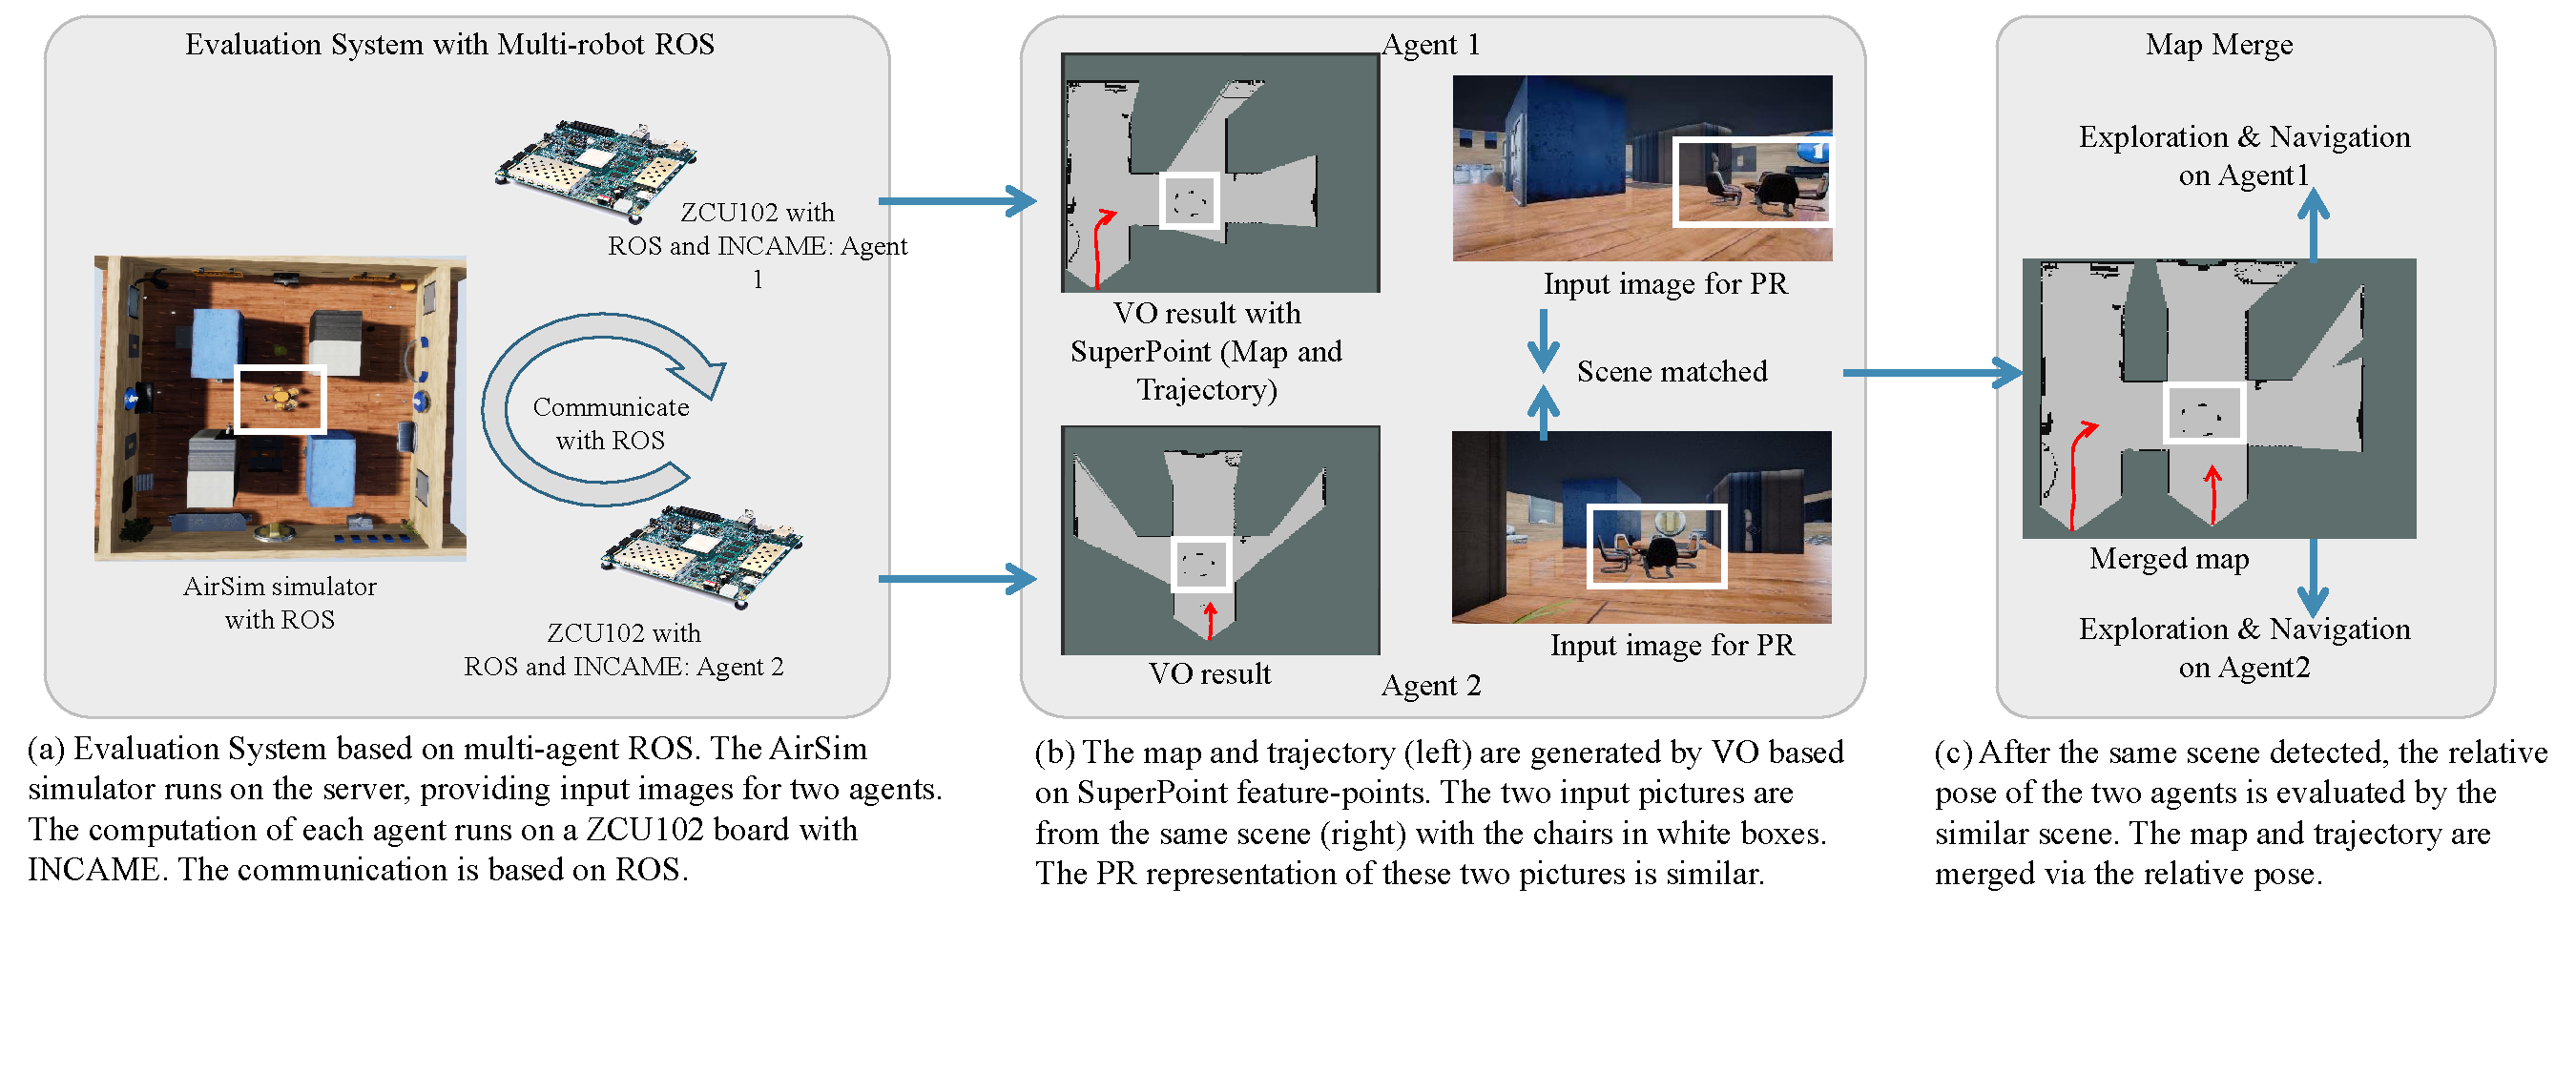
\includegraphics[width=0.99\linewidth]{fig/env.pdf}
  \caption{Multi-robot exploration: environment and results. }
  \label{fig:env}
\end{figure*}


% In this section, the evaluation of the instruction-based-interruption, hardware modules for FE post-processing, and the overall MR-Exploration system are presented and analyzed.



\subsection{ Experiment Setup }

The hardware-in-loop evaluate environment is illustrated in \Cref{fig:env}(a). There is a simulation server providing the simulation environment based on AirSim  ~\cite{shah2018airsim}, which is a high-fidelity visual and physical simulation for autonomous vehicles. The AirSim simulation server provides the camera data for each agent. Two Xilinx ZCU102 boards  ~\cite{zcu102}, with ZU9 MPSoC  ~\cite{MPSoC}, are responsible for the calculation of each agent. 
The components in \Cref{fig:maexp} for each agent are implemented in the ZCU102 board. The implementation of the FE (\textcircled{1} in \Cref{fig:maexp}), SuperPoint ~\cite{detone2018superpoint}), are introduced in former sections. GeM  ~\cite{radenovic2018fine} is used to implement the PR module (\textcircled{2}). GeM is a CNN-based method with ResNet101 \cite{he2016deep} as the backbone, and the post-processing of GeM calculates the 3-norm of the output featuremaps.
The VO module (\textcircled{3}) in the experiment is the PnP  ~\cite{LepetitMoreno-Noguer-EPnP} method, which is widely used in the feature-point based VO. 
% including the open source the ORB-SLAM  ~\cite{Mur-Artal:2017281}. 
The DOpt module (\textcircled{4}) is proposed in  ~\cite{Choudhary:2017e66} and also used in former distributed SLAM system ~\cite{cieslewski2018data}. 
The Map Merging  ~\cite{Andre2014} (\textcircled{5}), Exploration  ~\cite{8202319} (\textcircled{6}), and Navigation  ~\cite{tbd} (\textcircled{7}) in this work are provided by the ROS framework. 

The hardware resources are listed in \Cref{tab:hardware}. The hardware resources are provided by Vivado after hardware implementation. Vivado\cite{Vivado} is the development toolchain for MPSoC provided by Xilinx. The CNN backbone is calculated by the Angel-Eye CNN accelerator ~\cite{guo2017angel} on the FPGA side of ZCU102 (Programmable logic, PL side). The FE post-processing steps run on our proposed accelerators, also on the PL side. The PL side has 2 clock frequencies. The CNN accelerator and the IAU are running at 300MHz. The accelerator for FE post-processing is running at 200MHz. Compared with the CNN accelerator, IAU and FE post-processing use very little hardware resources.

% Table generated by Excel2LaTeX from sheet 'Sheet1'
\begin{table}[t]
  \centering
  % \setlength{\abovecaptionskip}{2pt}
  \caption{Hardware consumption of the proposed hardware}
% Table generated by Excel2LaTeX from sheet 'Sheet1'
\begin{tabular}{|c|c|c|c|c|}
  \hline
        & $\# DSP$ & $\# LUT$ & $\# FF$ & $\# BRAM$ \\
  \hline
  On-Board resource &   2520   &  274080      &  548160     & 912 \\
  \hline
  CNN accelerator &   1282   &  74569      &   171416    & 499 \\
  \hline
  IAU &   0   &  2268      &   4633    & 4 \\
  \hline
  FE post-processing & 25      &  17573     &   29115    & 10 \\
  \hline
  \end{tabular}%
  
  \label{tab:hardware}%
\end{table}%


\subsection{Virtual Instruction-based interrupt }

\subsubsection{ Interrupt response latency and extra cost}


We evaluate the latency to respond the interrupt and the performance degradation of different interrupt method. In MR-Exploration, only the low-priority PR task is interruptible, and the interrupt position is unpredictable. GeM  ~\cite{radenovic2018fine} is used to implement the PR module in the experiment.
The CNN backbone of the GeM is ResNet101  ~\cite{he2016deep}, which contains 101 convolution layers. The input shape of the CNN is $480 \times 640 \times 3$. The parallelism of the Angel-Eye is $Para_{height}=8$, $Para_{in}=16$, $Para_{out}=16$, i.e. each CALC instruction processes 8 lines from 16 input channels to 16 output channels. 
% Thus, we randomly selected some interrupt locations inside the PR network.

As shown in \Cref{fig:scatter1024}(a), the latency to respond the interrupt in CPU-like method consists of the time to finish current executing instruction and the data backup time ($t_{latency} = t_1+t_2$) for the on-chip data/weights caches (totally 2.2MB). The latency in layer-by-layer interrupt is the time to finish current layer. The latency of our virtual-instruction-based method is the time to finish current executing instruction and the backup time for the calculated output results. 

The cost of CPU-like interrupt is the data transfer time of all the on-chip caches (totally 2.2MB) to/from DDR ($t_{cost} = t_2+t_4$). The cost of virtual-instruction-based method is only the recovery of the input/weights from DDR to on-chip caches ($t_{cost} = t_4$). There is no extra cost for the layer-by-layer interrupt.

% For a precise evaluation the CNN run time, we record the clock cycles of the beginning and end of each instruction. The time of the interrupt response latency and the total cost in the following evaluation is calculated from the clock cycles and the clock frequence.


We randomly sample 12 positions of the ResNet101 CNN backbone. The interrupt response latency and the extra time cost for different implementation of interrupt at the positions are listed in \Cref{fig:scatter1024}(b).
The CPU-like interrupt consumes the most extra cost ($t_{cost}$). Though the layer-by-layer interrupt consumes no extra time, the latency is much higher than our virtual-instruction-based interrupt. 
This is because the layer-by-layer interrupt need to wait for completion of a layer. The performance at same interrupt position in our proposed virtual interrupt can interrupt inside a layer, with lower latency.

Furthermore, though the network structures differ between different CNNs, the convolutional layers, which are the basic component in CNN, are similar between different CNNs. INCAME monitors the running status inside each layer, and the interrupt respond latency and extra cost are only relevant to the currently operating layer. Thus, the latency and cost are also similar between different CNNs. In conclusion, the process for different CNN tasks are similar, and the cost of different tasks are similar.

\subsubsection{ Time comparison between $t_1$ and $t_2$ }

As described in \Cref{sec:virtualinstr}, the Layer-By-Layer interrupt method do not need to backup data before interruption ($t_2 = 0$). Though our Virtual-Instruction method (VI method) need to spend time to backup the final results, which are already generated yet not stored to DDR ($t_2$). However, compared with computation, the time of data backup ($t_2$) is short. We list the backup time and the convolution time ($t_1$) at some of the interrupt position in \Cref{fig:scatter1024}(b), with different featuremap shape, kernel size, and input/output channels. $H$, $W$ are the height, width of input featuremaps. $Ch_{in}$, $Ch_{out}$ are the number of input and output channels. The time of backup and calculation is listed in $Backup$ and $Conv$ columns. The ratio of backup and calculation are listed in the last column. The backup operation only consumes less than 20\% of the calculation time. For the first layer (first line of \Cref{tab:timecompare}). The input channels number is too small, so the calculation time is also short. Therefore, the backup time has reached half of the calculation time. 

% Table generated by Excel2LaTeX from sheet 'Sheet4'
\begin{table}[t]
  \centering
  % \footnotesize
  \caption{Time comparison between data backup and calculation}
    \begin{tabular}{|c|c|c|c|c|c|c|c|}
    \hline
    \multirow{2}[2]{*}{$H$} & \multirow{2}[2]{*}{$W$} & \multirow{2}[2]{*}{$Ch_{in}$} & \multirow{2}[2]{*}{$Ch_{out}$} & Kernel & Backup & Conv  & \multirow{2}[2]{*}{$\frac{Backup}{Conv}$} \bigstrut[t]\\
          &       &       &       & Size  & ($t_2$,$us$)  & ($t1$,$us$)  &  \\
    \hline
    480   & 640   & 3     & 64    & $7 \times 7$ & 26.29  & 52.38  & 50.2\% \\
    \hline
    120   & 160   & 128   & 128   & $3 \times 3$ & 8.77  & 41.18  & 21.3\% \\
    \hline
    30    & 40    & 1024  & 2048  & $1 \times 1$ & 1.25  & 8.75  & 14.3\% \\
    \hline
    30    & 40    & 512   & 512   & $3 \times 3$ & 1.42  & 39.36  & 3.6\% \\
    \hline
    16    & 20    & 512   & 512   & $3 \times 3$ & 0.75  & 20.16  & 3.8\% \\
    \hline
    \end{tabular}%
  \label{tab:timecompare}%
\end{table}%




\subsubsection{ Additional data transfer for the virtual instructions. }
% The worst latency of the layer-by-layer interrupt reaches 10 ms, because the interrupt occurs at the beginning of the second layer, which is the most time-consuming layer (10ms). The layer-by-layer interrupt need to wait for the finish of this layer. The performance at same interrupt position in our proposed virtual interrupt is not significantly different from that of other positions. Our method is significantly better than others at worst case. 

The extra virtual instruction number is listed in \Cref{tab:instrnum}. Compared to the normal instruction transfer, the volume of virtual instructions is less than 10\%. The performance degradation brought by the extra virtual instructions is negligible. 
We are here to remind the readers that the processing of the low-priority PR task can be interrupted twice or more. And in that case, the PR task is interrupted by several FE tasks.



% DPU first calculates all channels of the output row before calculating the next rows. As the number of channels increases, the number of weights requiring recovery increases squarely. However, the size of the input data to be restored and the output results to be backed up remains basically the same.


% % Table generated by Excel2LaTeX from sheet 'Sheet2'
% \begin{table}[t]
%   \small
%   \centering
%   \caption{Worst latency different interrupt positions.}
%     % Table generated by Excel2LaTeX from sheet 'Sheet2'
% \begin{tabular}{|c|c|c|c|c|c|}
%   \hline
%         & Backup  & Recovery & CPU-like & layer-by-layer & Virtual Instr. \bigstrut[t]\\
%         & (KB)  & (KB)  &  Latency (ms) & Latency (ms)   & Latency (ms) \bigstrut[b]\\
%   \hline
%   Pose 1 &       &       &       &      &  \bigstrut\\
%   \hline
%   Pose 2 &       &       &       &      &  \bigstrut\\
%   \hline
%   Pose 3 &       &       &       &      &  \bigstrut\\
%   \hline
%   CPU-Like & 4000  & 4000  &     &       & <1 \bigstrut\\
%   \hline
%   Serial & -     & -     &     &   & - \bigstrut\\
%   \hline
%   \end{tabular}%
  
  
%   \label{tab:anywhere}%
% \end{table}%


\begin{figure}[t]
  \centering
%   \vspace{-0.1cm} 
  % \setlength{\abovecaptionskip}{0cm} 
%   \setlength{\belowcaptionskip}{-0.05cm} 
  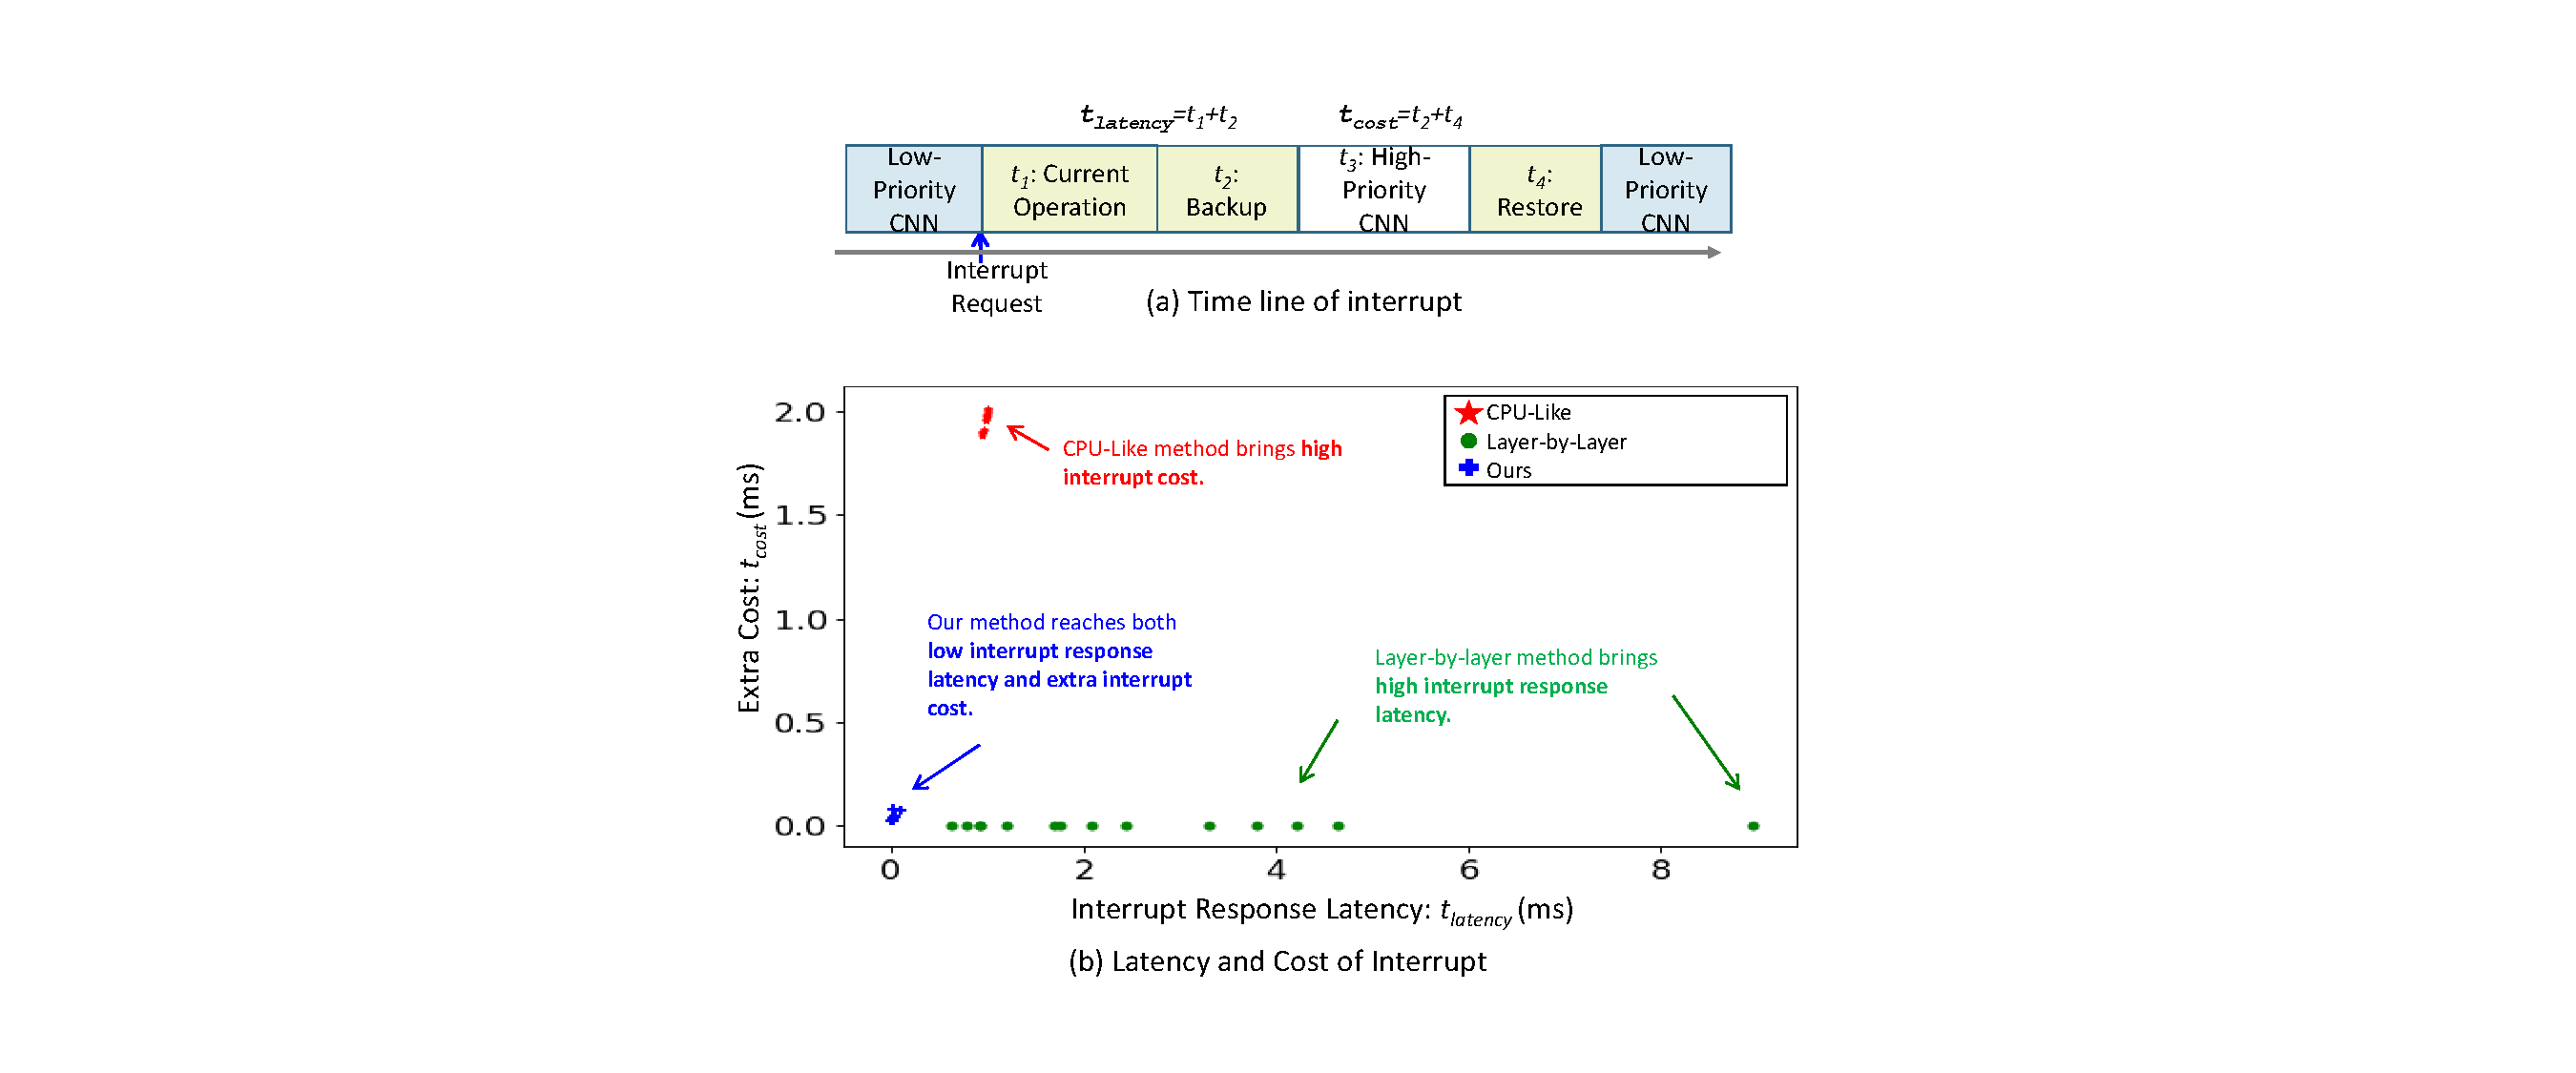
\includegraphics[width=0.99\linewidth]{fig/PRresult.pdf}
  \caption{The interrupt response latency \& extra time cost.}
  \label{fig:scatter1024}
\end{figure}
% Table generated by Excel2LaTeX from sheet 'Sheet2'
\begin{table}[t]
  \small
  \centering
  % \setlength{\abovecaptionskip}{2pt}
  \caption{The instruction number of the interruptible PR network (backbone). }
    % Table generated by Excel2LaTeX from sheet 'Sheet2'
\begin{tabular}{|c|c|c|c|c|c|}
  \hline
         & Instr.  & Instr. & Execute \\
        & Number   & volume (MB) & Time (ms) \\
  \hline
  Original ISA   &      364032      & 4.36 & 186.0 \\
  \hline
  VI-ISA   &     400243    & 4.80 & 186.4 \\
  \hline
  \end{tabular}%
  \label{tab:instrnum}%
\end{table}%



% % Table generated by Excel2LaTeX from sheet 'Sheet1'
% \begin{table}[t]
%     \centering
%     \caption{Interrupt after complete results vs Interrupt anywhere}
% % Table generated by Excel2LaTeX from sheet 'Sheet2'
% \begin{tabular}{|c|c|c|c|c|c|}
%   \hline
%   \multicolumn{1}{|c}{} &       & \multicolumn{1}{c|}{Backup } & \multicolumn{1}{c|}{Recovery} & Exe time & Performance \bigstrut[t]\\
%   \multicolumn{1}{|c}{} &       & \multicolumn{1}{c|}{data (KB)} & \multicolumn{1}{c|}{ data (KB)} & (ms)  & Reduce \bigstrut[b]\\
%   \hline
%   \multicolumn{1}{|p{3.315em}|}{Inter } & \multicolumn{1}{p{3.69em}|}{AfterSave} &       &       &       &  \bigstrut\\
%   \cline{2-6}\multicolumn{1}{|p{3.315em}|}{position 1} & Anyware &       &       &       &  \bigstrut\\
%   \hline
%   \multicolumn{1}{|p{3.315em}|}{Inter } & \multicolumn{1}{p{3.69em}|}{AfterSave} &       &       &       &  \bigstrut\\
%   \cline{2-6}\multicolumn{1}{|p{3.315em}|}{ position 2} & Anyware &       &       &       &  \bigstrut\\
%   \hline
%   \multicolumn{1}{|p{3.315em}|}{Inter } & \multicolumn{1}{p{3.69em}|}{AfterSave} &       &       &       &  \bigstrut\\
%   \cline{2-6}\multicolumn{1}{|p{3.315em}|}{position 3} & Anyware &       &       &       &  \bigstrut\\
%   \hline
%   \multicolumn{2}{|p{7.005em}|}{CPU-Like} &       &       &       &  \bigstrut\\
%   \hline
%   \multicolumn{1}{|c}{} &       & \multicolumn{1}{c|}{Instruction} & \multicolumn{1}{c|}{Latency} & Exe time & Performance \bigstrut[t]\\
%   \multicolumn{1}{|c}{} &       & \multicolumn{1}{c|}{ (KB)} & \multicolumn{1}{c|}{(ms)} & (ms)  & Reduce \bigstrut[b]\\
%   \hline
%   \multicolumn{1}{|c|}{No} & \multicolumn{1}{p{3.69em}|}{Origin} &       &       &       & 0 \bigstrut\\
%   \cline{2-6}\multicolumn{1}{|c|}{ Interrupt} & \multicolumn{1}{p{3.69em}|}{After results} &       &       &       &  \bigstrut\\
%   \cline{2-6}      & Anyware &       &       &       &  \bigstrut\\
%   \hline
%   \end{tabular}%
  
%     \label{tab:anywhere}%
%   \end{table}%



% \subsection{ **Place Recognition With the CNN accelerator }

% In this section, we evaluate the accuracy of the PR network on the CNN accelerator with fixed-point number. 

% \begin{figure}[t]
%     \centering
%     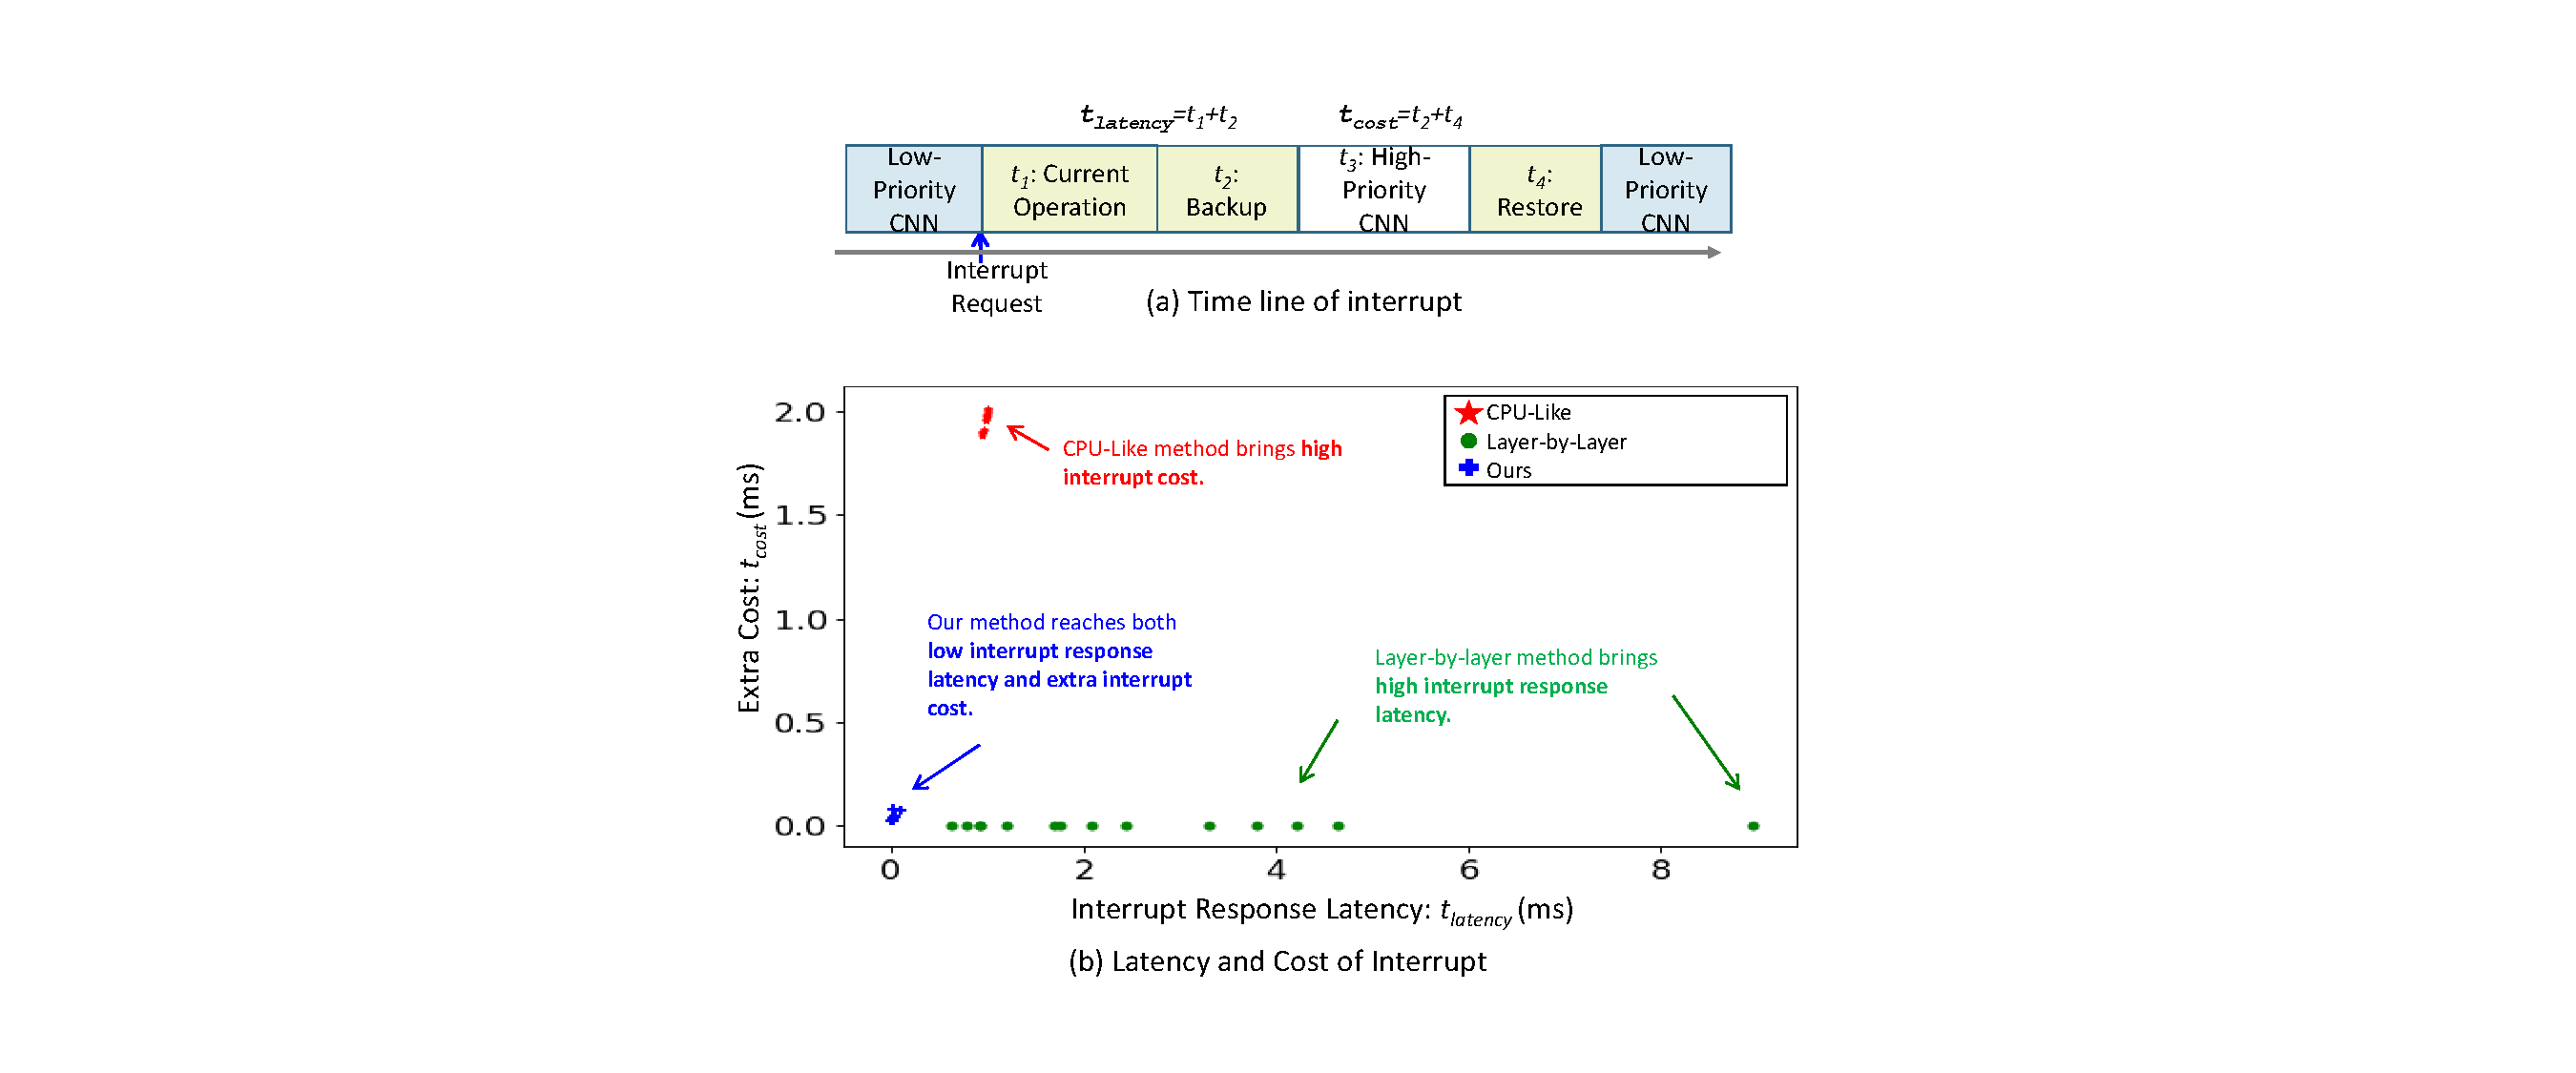
\includegraphics[width=0.8\linewidth]{fig/PRresult.pdf}
%     \caption{Precision-Recall curve on Citycenter dataset}
%     \label{fig:PRcurve}
% \end{figure}

% % We want to prove two things in our experiment. 1) The GeM network used in our work outperforms other networks such as NetVLAD. 2) The quantization of GeM CNN backbone don't bring about much drop in accuracy. 
% We test 3 networks, a) float-point GeM, b) float-point NetVLAD, c) fixed-point GeM on Citycenter dataset [??] and draw the Precision-Recall curve. The result is shown in figure \ref{fig:PRcurve}. It's clear that after quantization, the accuracy slightly reduced and still outperforms the float-point NetVLAD network  ~\cite{arandjelovic2016netvlad}, especially at higher recall, which is used in the MA-Exploration system.

% \begin{figure}[t]
%   \centering
%   \includegraphics[width=0.8\linewidth]{fig/example.eps}
%   \caption{Example of GeM performance.}
%   \label{fig:gem_exp}
% \end{figure}

% Figure \ref{fig:gem_exp} shows an example in our similation environment. Picture 1 and Picture 2 is photoed in the same place and Picture 3 is photoed in another place. The computed similarity of Picture 1 and 2 is 0.8887, apparently larger than the similarity of Picture 2 and 3 (0.8046).

% \subsubsection{efficiency}

% \begin{table}
%     \label{tab:gem_eff}
%     \centering 
%     \caption{running time comparison of each operation in PR}
%     \begin{tabular}{|c|c|c|}
% 				\hline
%               & CPU & CPU+FPGA \\
%         \hline
%            &   48 ms &   42 ms \\
% 			  \hline
%     \end{tabular}
%   \end{table}

% As illustrated in section \ref{sec:hardsoftcodesign}, we do optimization on GeM backend processing, i.e., the GeM pooling layer. We compare running time before and after optimization, and the result is shown in table \ref{tab:gem_eff}. After optimization, the total time reduces by 12.5\%.


\subsection{ FE Evaluation }

We evaluate the performance of the SuperPoint network in VO on the $TUM$ dataset ~\cite{sturm12iros}. We evaluate SuperPoint against two well-known handcrafted FE systems: SIFT ~\cite{Lowe-478} and ORB ~\cite{Mur-Artal:2017281}. 
We also evaluate the performance after optimization. 
We extract a maximum of 200 feature-points at a $480\times640$ input resolution. 
We perform nearest neighbor matching from descriptors in adjacent frames with a maximum allowable distance $d_m$. $d_m$ is not the same in three FE systems because these three descriptors are different. In PS side, we use an OpenCV implementation (solvePnP()) with all the matches to compute the transform matrix  ~\cite{LepetitMoreno-Noguer-EPnP}, and use Bundle Adjustment (BA) to optimize results  ~\cite{TriggsMclauchlan-Bundle-Adjustment}. 
% All the computation of this experiment is all done on the CPU except CNN of SuperPoint. 

Results are shown in \Cref{tab:VO}. In terms of accuracy, SuperPoint outperforms ORB and SIFT. Our optimizations, including fixed-point quantization, and post-processing acceleration, do not introduce a large loss of accuracy. 
% In terms of calculation speed, SuperPoint takes less time than Sift, and is equivalent to ORB. 
% After optimization, the running speed of SuperPoint is increased by $4\times$, making real-time processing possible.

\begin{table}[t]
  \centering
  % \setlength{\abovecaptionskip}{2pt}
  \caption{Running time comparison of each FE operation}
    \begin{threeparttable}
% Table generated by Excel2LaTeX from sheet 'Sheet2'
\begin{tabular}{|c|c|c|c|c|c|}
  \hline
             &CNN$^*$ &    Softmax &        NMS &       Rank &  Norm \\
  \hline
         CPU & \multirow{2}{*}{24ms} &      31ms &       27ms &       0.97ms &       42ms \\
  \cline{1-1} \cline{3-6}
    Ours & \multirow{2}{*}{} &    1.97ms &      0.7ms &     0.12ms &     1.44ms \\
  \hline
  \end{tabular} 
  \small
\begin{tablenotes}
   \item[*] CNN backbone runs on the accelerator.  
\end{tablenotes}
    \end{threeparttable}
  
  \label{tab:optimization}%
\end{table}%

We compare the running time of each operation in SuperPoint post-processing before and after the optimization. Results are shown in \Cref{tab:optimization}. The running time of post-processing is reduced by more than $20\times$. There is a certain gap between the experimental results of the acceleration effect and the theoretical derivation in \Cref{subsec:FEopt}. The possible reason is that the CPU needs time to schedule the FPGA accelerator.

\begin{table}[t]
  \centering
  % \setlength{\abovecaptionskip}{2pt} 
  \caption{ Accuracy and running time results on the TUM ~\cite{sturm12iros} dataset  }
  \footnotesize
  \begin{threeparttable}
% Table generated by Excel2LaTeX from sheet 'Sheet2'
\begin{tabular}{|c|c|c|c|} 
  \hline
        & RPE$^2$(m/s) & ATE$^3$(m)  & Running time(ms) \bigstrut\\
  \hline
  SIFT  ~\cite{Lowe-478}  & 0.0319  & 0.4219 & 2397  \bigstrut\\
  \hline
  ORB  ~\cite{Mur-Artal:2017281}  & 0.0577  & 0.6105 & 229  \bigstrut\\
  \hline
  Original SuperPoint  ~\cite{detone2018superpoint} & 0.0280  & 0.3671 & 259  \bigstrut\\
  \hline
  Our Fixed SuperPoint  & 0.0283  & 0.3976 & 59  \bigstrut\\
  \hline
  \end{tabular}%
  

\begin{tablenotes}
  \item[1] RPE is the mean Relative Pose Error to indicate the translational drift per second. The less, the better.
  \item[2] ATE is the root mean square Absolute Trajectory Error to indicate the translational drift of the entire trajectory. The less, the better.
\end{tablenotes}
    \end{threeparttable}
  \label{tab:VO}%
\end{table}%

% \vspace*{-2mm}
\subsection{ ROS based MR-Exploration }

The results of the Multi-Robot Exploration based on INCAME is shown in \Cref{fig:env}. The space in the AirSim~\cite{shah2018airsim} for the robots to explore is shown in \Cref{fig:env}(a). It is a simple rectangle area with four different pillars, and some chairs at the center (in the white box).  \Cref{fig:env}(b) shows how PR works for map merging. The FE and VO of each agent produce the local map and trajectory on each ZCU102 board. When the PR threads on different agents find out a similar scene, the relative pose of the two agents at the similar scene is calculated. The map and the trajectory is merged with the calculated relative pose, as shown in \Cref{fig:env}(c).

In this example, the FE and PR are both executed on the same Angel-Eye accelerator. The frequency of the input camera is 20fps, and each input frame is fed to the FE, and FE module would take up accelerator. While the CPU process VO with the feature-points from FE, the accelerator can switch to process the low-priority PR task. Because the executing time of VO varies, the time to finish a PR task is different. In this example, the time from the beginning of a PR to its end is 320$\sim$500 ms. Thus, the PR process one key frame every 7$\sim$10 input frames.

\section{Conclusion}
\label{sec:conclusion}

In this paper, we propose an interruptible CNN accelerator and a deployment framework, INCAME, for multi-robot exploration. 
With the help of the virtual-instruction-based interrupt method, the CNN accelerator can switch between different CNN tasks with low interrupt response latency and low extra cost. Note that the development of CPU task scheduling evolved from single-core multi-tasking to multi-core multi-tasking. Similarly, INCAME currently focuses on interrupt support for single-core multi-tasking. We plan to investigate the multi-core multi-tasking for CNN accelerators as part of future work.
INCAME only needs to modify the instruction fetch module to IAU in hardware. Thus, it is easy to extend to handle other instruction-driven accelerators.
Therefore, with the help of INCAME, the independent software in ROS can access the accelerator without hardware resources conflicts, on various CNN accelerators.
INCAME also accelerates the time-consuming post-processing operations like SoftMax, NMS, normalization.
So that the ROS-based MR-Exploration can achieve real-time performance on embedded FPGA. In the future, more robotic algorithms, such as DOpt, Exploration, and Navigation, can be implemented on hardware and included in INCAME, to gain better energy efficiency and achieve better real-time performance. The multi-task supporting multi-core CNN accelerators can also be included in our future work.

% asWith the help of the virtual-instruction based method,

% use section* for acknowledgment
% \section*{Acknowledgment}
% This work is supported by National Key Research and Development Program of China (No. 2017YFA0207600 ), National Natural Science Foundation of China (No. U19B2019, 61832007 ), Tsinghua EE Xilinx AI Research Fund, Beijing National Research Center for Information Science and Technology (BNRist), and Beijing Innovation Center for Future Chips.

% Can use something like this to put references on a page
% by themselves when using endfloat and the captionsoff option.
\ifCLASSOPTIONcaptionsoff
  \newpage
\fi



% trigger a \newpage just before the given reference
% number - used to balance the columns on the last page
% adjust value as needed - may need to be readjusted if
% the document is modified later
%\IEEEtriggeratref{8}
% The "triggered" command can be changed if desired:
%\IEEEtriggercmd{\enlargethispage{-5in}}

% references section

% can use a bibliography generated by BibTeX as a .bbl file
% BibTeX documentation can be easily obtained at:
% http://mirror.ctan.org/biblio/bibtex/contrib/doc/
% The IEEEtran BibTeX style support page is at:
% http://www.michaelshell.org/tex/ieeetran/bibtex/
%\bibliographystyle{IEEEtran}
% argument is your BibTeX string definitions and bibliography database(s)
%\bibliography{IEEEabrv,../bib/paper}
%
% <OR> manually copy in the resultant .bbl file
% set second argument of \begin to the number of references
% (used to reserve space for the reference number labels box)
\bibliographystyle{IEEEtran}
\bibliography{src/fpgaslam}
% biography section
% 
% If you have an EPS/PDF photo (graphicx package needed) extra braces are
% needed around the contents of the optional argument to biography to prevent
% the LaTeX parser from getting confused when it sees the complicated
% \includegraphics command within an optional argument. (You could create
% your own custom macro containing the \includegraphics command to make things
% simpler here.)
%\begin{IEEEbiography}[{\includegraphics[width=0.6in,height=0.8in,clip,keepaspectratio]{mshell}}]{Michael Shell}
% or if you just want to reserve a space for a photo:

% \begin{IEEEbiography}{Michael Shell}
% Biography text here.
% \end{IEEEbiography}

% % if you will not have a photo at all:
% \begin{IEEEbiographynophoto}{John Doe}
% Biography text here.
% \end{IEEEbiographynophoto}

% % insert where needed to balance the two columns on the last page with
% % biographies
% %\newpage

% \begin{IEEEbiographynophoto}{Jane Doe}
% Biography text here.
% \end{IEEEbiographynophoto}


\begin{IEEEbiography}[{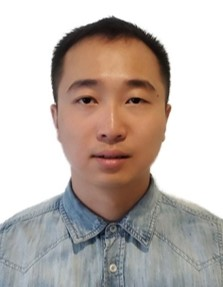
\includegraphics[width=0.6in,height=0.8in,clip,keepaspectratio]{fig/yujc.jpg}}]{Jincheng Yu}
  \footnotesize
  received his B.S. degree in electronic engineering department of Tsinghua University, Beijing, China, in 2016. He is currently pursing his Ph.D degree in electronic engineering department of Tsinghua University. His research mainly focues on deep learning acceleration and the hardware architecture for robot systems.
\end{IEEEbiography}



\begin{IEEEbiography}[{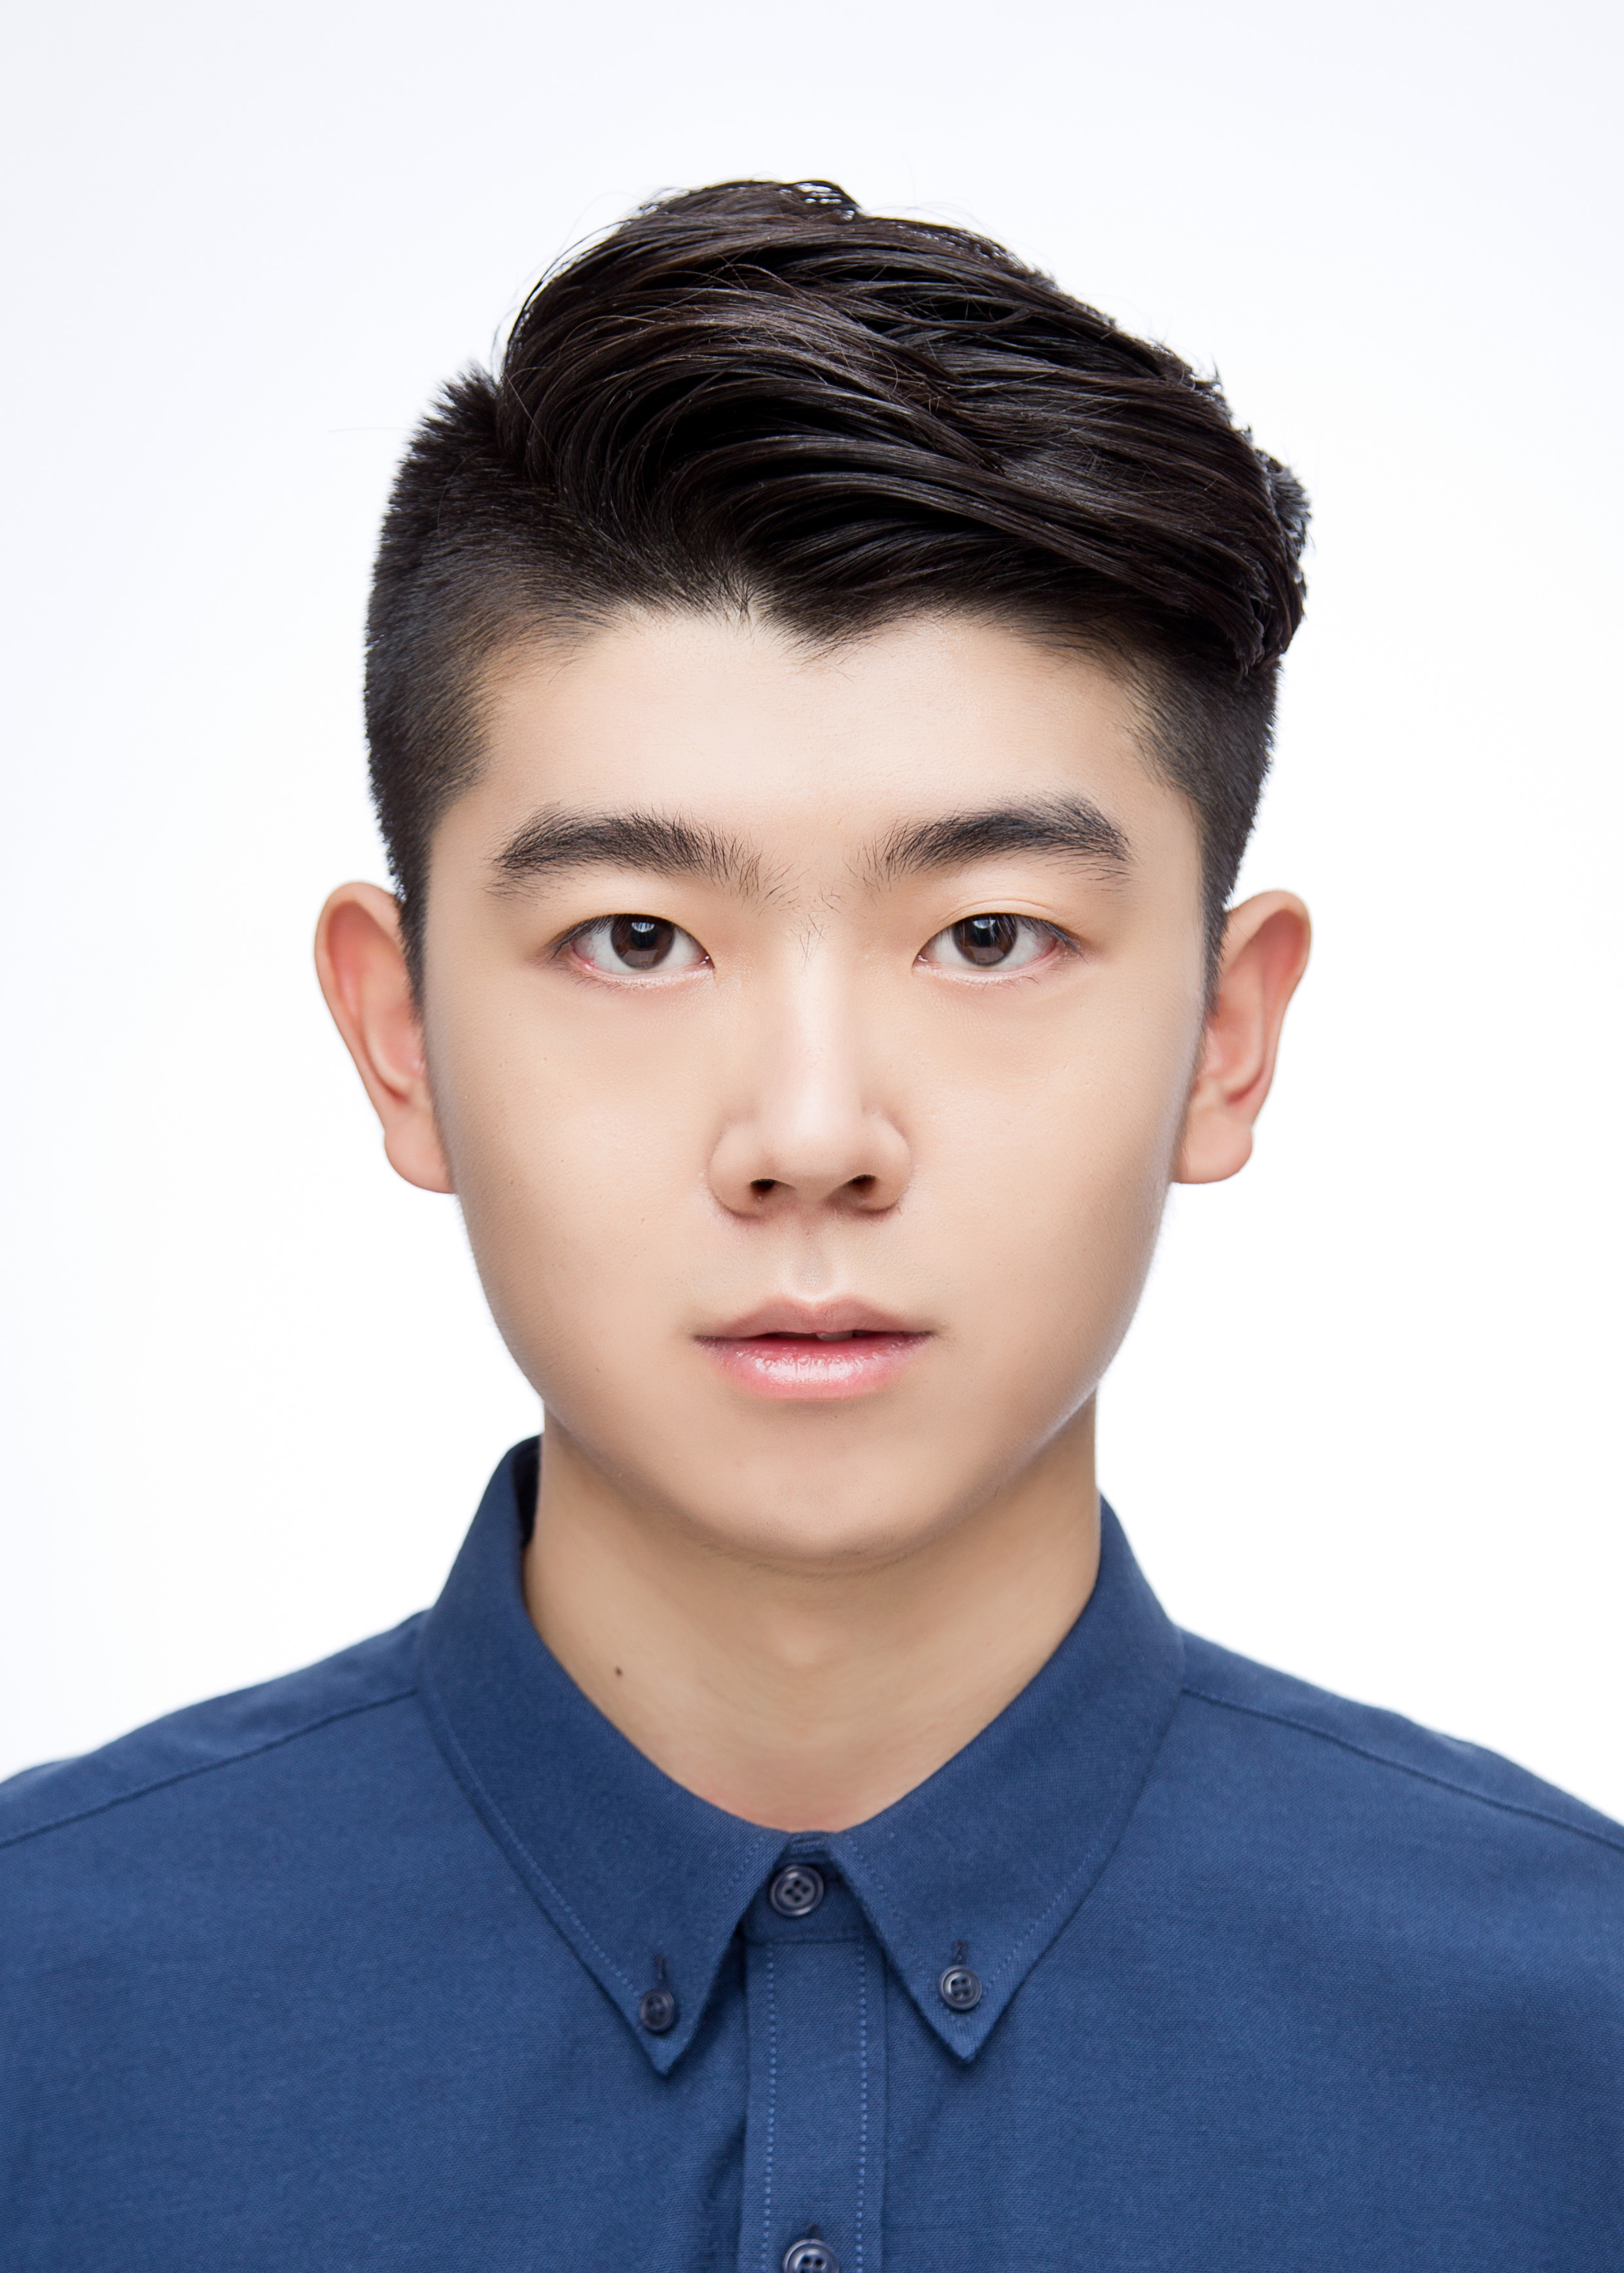
\includegraphics[width=0.6in,height=0.8in,clip,keepaspectratio]{fig/xuzhl.jpg}}]{Zhilin Xu}
  \footnotesize
  received his B.S. degree in College of Electronic Engineering from Beijing University of Posts and Telecommunications, Beijing, in 2018. He is currently pursuing his M.S. degree in the Department of Electronic Engineering, Tsinghua University, Beijing. His research mainly focuses on deep learning acceleration and the hardware architecture for robot systems. 
\end{IEEEbiography}


\begin{IEEEbiography}[{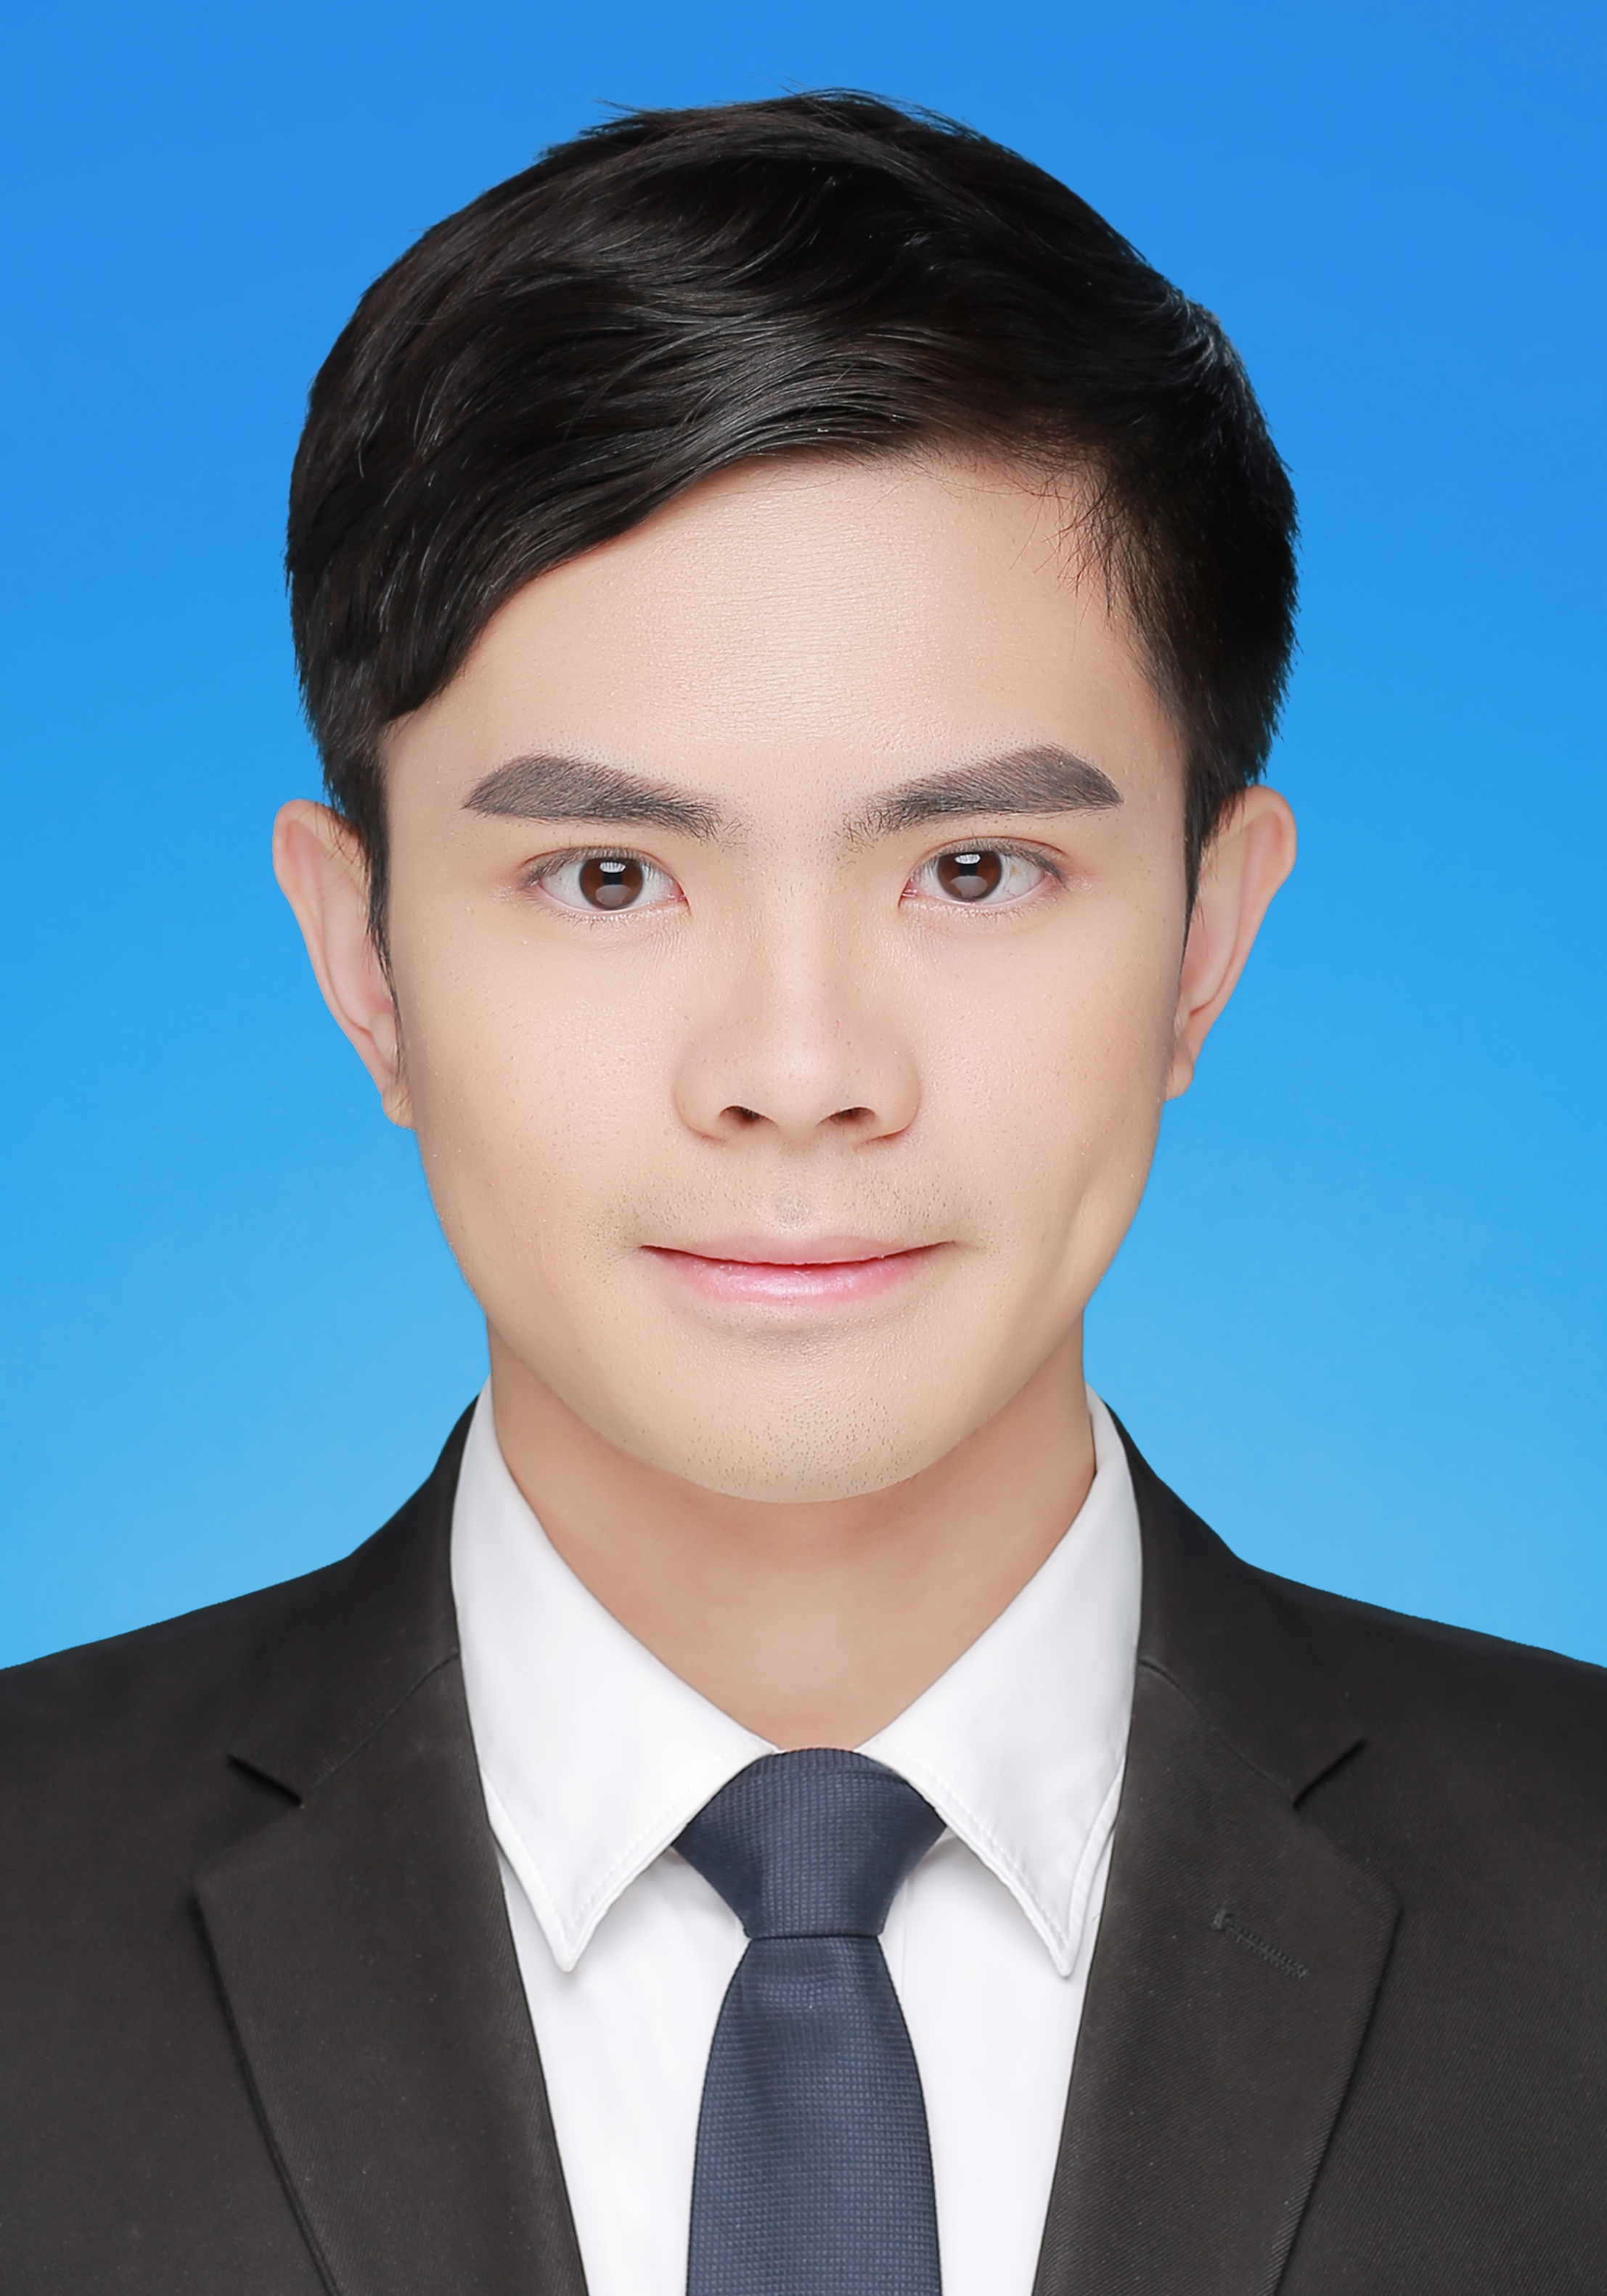
\includegraphics[width=0.6in,height=0.8in,clip,keepaspectratio]{fig/zengsl.jpg}}]{Shulin Zeng}
  \footnotesize
  received his B.S. degree in electronic engineering department of Tsinghua University, Beijing, China, in 2014. He is currently pursing his Ph.D degree in electronic engineering department of Tsinghua University. His research mainly focus on software-hardware co-design for deep learning and virtualization in the cloud.
\end{IEEEbiography}


\begin{IEEEbiography}[{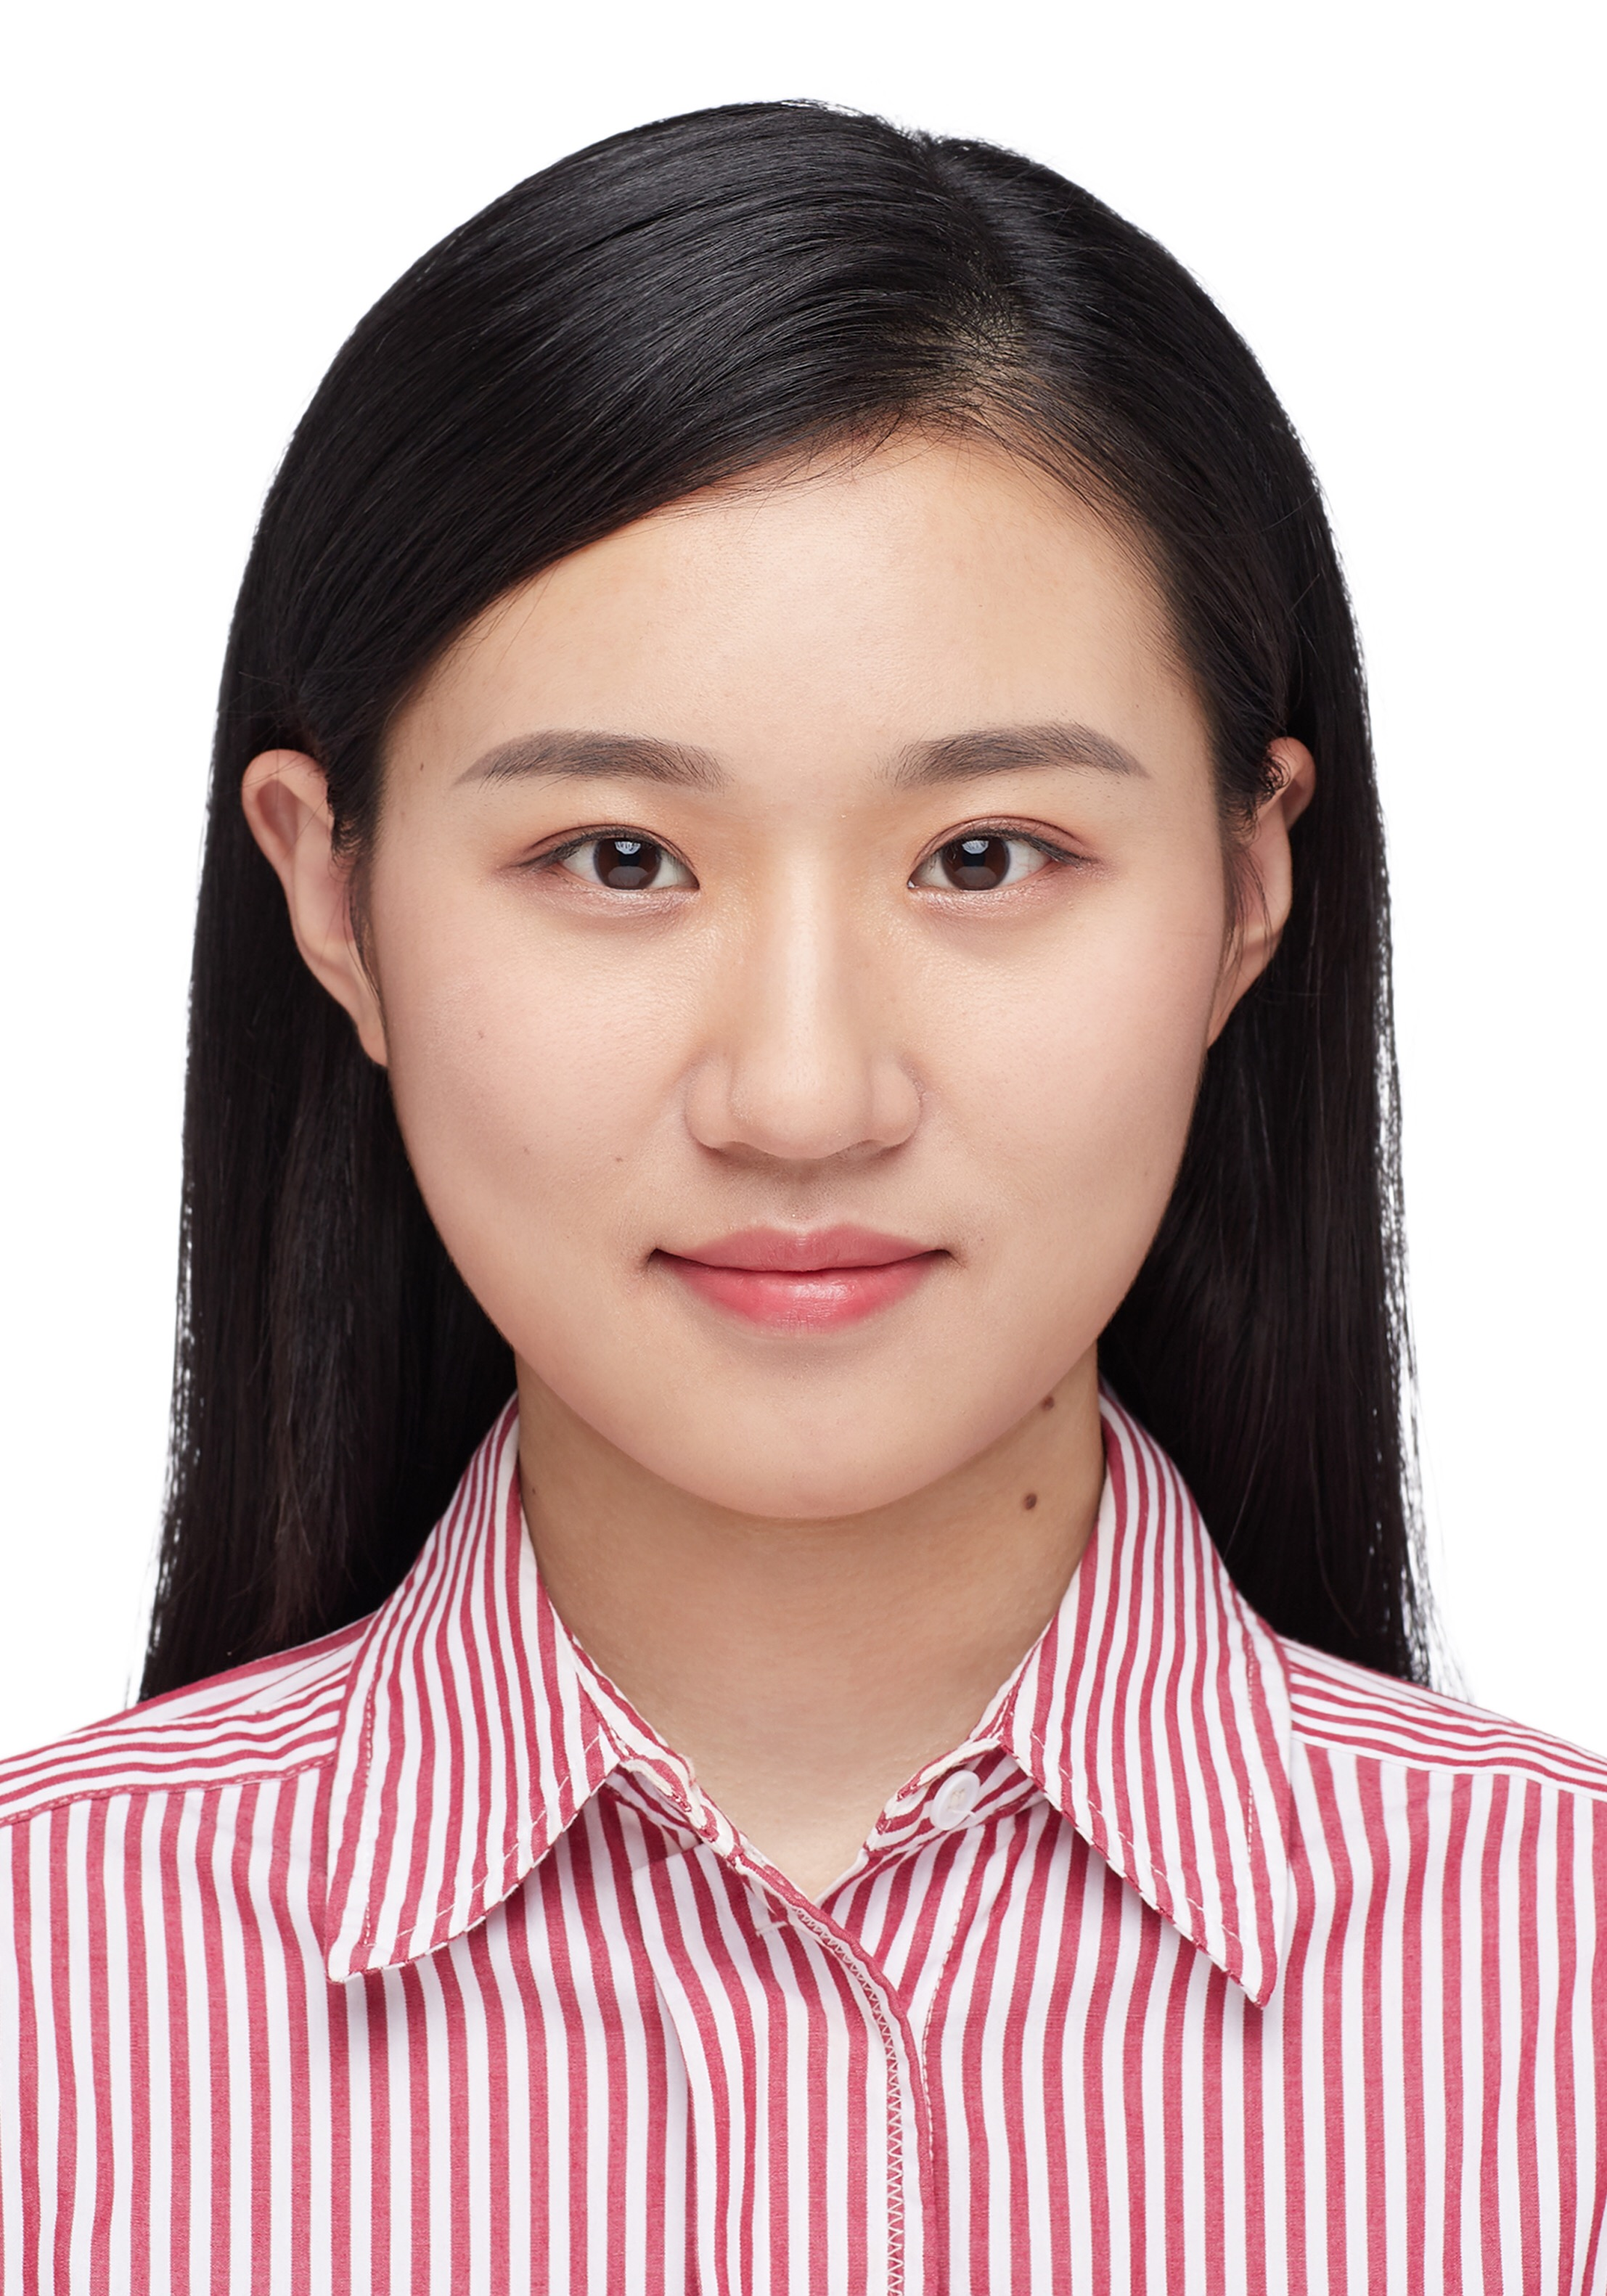
\includegraphics[width=0.6in,height=0.8in,clip,keepaspectratio]{fig/yuchao.jpg}}]{Chao Yu}
  \footnotesize
  received her B.S. degree in School of Automation of Beijing Institute of Technology, Beijing, China in 2016. In 2019, she received Master degree in Department of mechanical engineering of Tsinghua University. Now she is pursing the Ph.D degree in Department of Electric Engineering of Tsinghua University. Her research mainly focuses on SLAM, Multi-agent Reinforcement Learning (MARL), and Robotics.
\end{IEEEbiography}

\begin{IEEEbiography}[{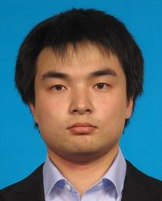
\includegraphics[width=0.6in,height=0.8in,clip,keepaspectratio]{fig/qjt.png}}]{Jiantao Qiu}
  \footnotesize
  received the B.S. degree in electronic engineering from Tsinghua University, Beijing, China, in 2015. He is currently pursuing the Ph.D. degree with the Center for Brain-Inspired Computing Research, Tsinghua University, Beijing. His current research interests include computing architecture, reinforcement learning, and system scheduling.
\end{IEEEbiography}


\begin{IEEEbiography}[{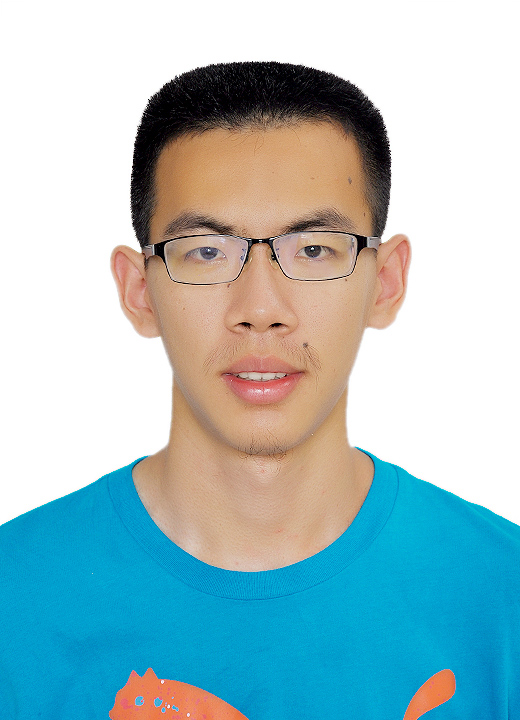
\includegraphics[width=0.6in,height=0.8in,clip,keepaspectratio]{fig/scy.jpg}}]{Chaoyang Shen}
  \footnotesize
  is a fourth year student in electronic enginnering deparment of Tsinghua University, Beijing, China. He is going to pursue his bachelor's degree in Tsinghua Shenzhen International Graduate School, Shenzhen, China. His research mainly focuss on  robotic vision.
\end{IEEEbiography}

\begin{IEEEbiography}[{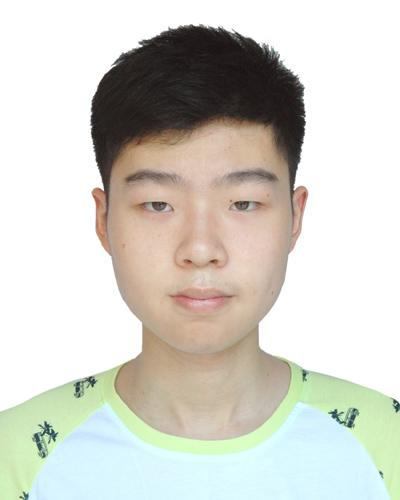
\includegraphics[width=0.6in,height=0.8in,clip,keepaspectratio]{fig/xuyf.jpg}}]{Yuanfan Xu}
  \footnotesize
  is currently pursuing his B.S. degree in electronic engineering in Tsinghua University, Beijing. His research interests include multi-agent reinforcement learning,  the hardware architecture for robot systems and SLAM.
\end{IEEEbiography}

\begin{IEEEbiography}[{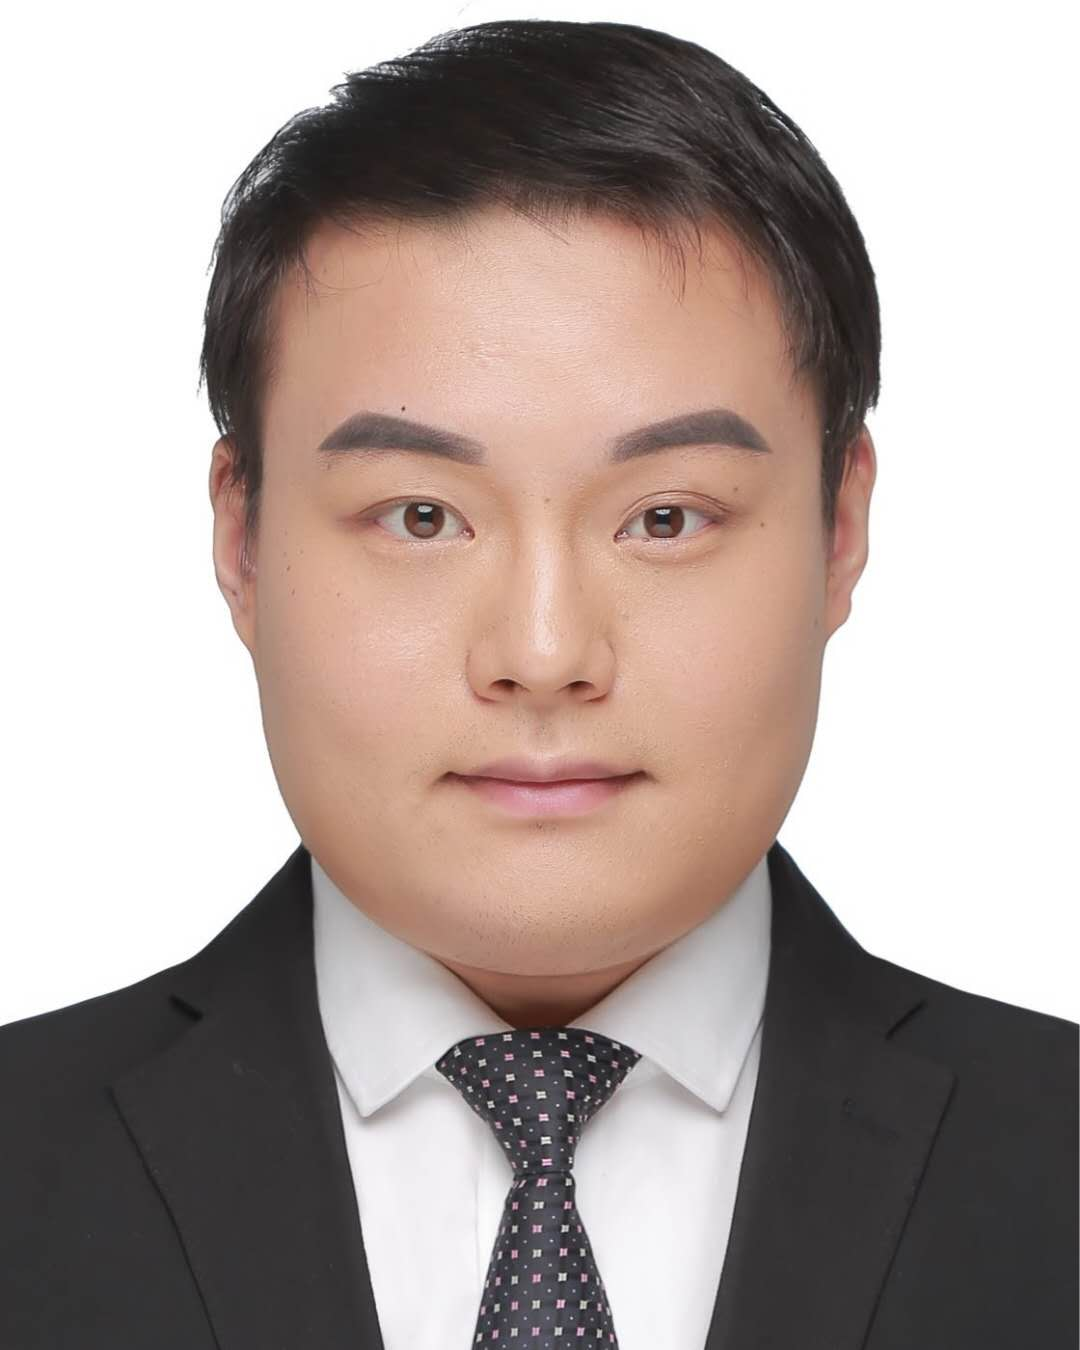
\includegraphics[width=0.6in,height=0.8in,clip,keepaspectratio]{fig/dgh.jpg}}]{Guohao Dai}
  \footnotesize
  received his B.S. degree in 2014 and Ph.D degree (with honor) in 2019 from Tsinghua University, Beijing. He is currently a PostDoc Researcher at the Department of Electronic Engineering, Tsinghua University, Beijing. His current research interests include acceleration of large-scale graph processing on hardware and emerging devices, and virtualization techniques in the cloud. He has received Best Paper Award in ASPDAC 2019, and Best Paper Nomination in DATE 2018.
\end{IEEEbiography}

\begin{IEEEbiography}[{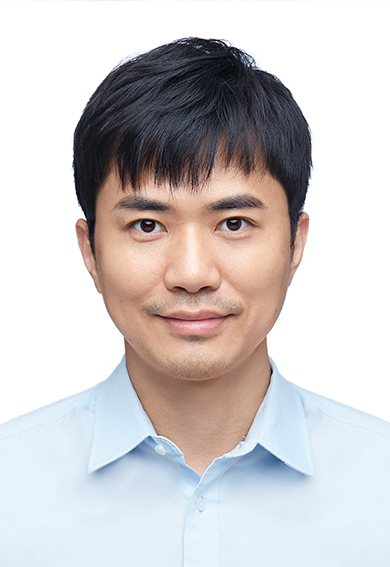
\includegraphics[width=0.6in,height=0.8in,clip,keepaspectratio]{fig/wangyu.jpg}}]{Yu Wang}
  \footnotesize
   (S’05-M’07-SM’14) received the BS and   PhD (with honor) degrees from Tsinghua University,   Beijing, in 2002 and 2007. He is currently a tenured   professor with the Department of Electronic Engineering, Tsinghua University. His research interests   include brain inspired computing, application specific hardware computing, parallel circuit analysis,   and power/reliability aware system design methodology. He has authored and coauthored more than 200   papers in refereed journals and conferences. He has   received Best Paper Award in ASPDAC 2019, FPGA   2017, NVMSA 2017, ISVLSI 2012, and Best Poster Award in HEART 2012   with 9 Best Paper Nominations (DATE18, DAC17, ASPDAC16, ASPDAC14,   ASPDAC12, 2 in ASPDAC10, ISLPED09, CODES09). He is a recipient of   DAC under 40 innovator award (2018), IBM X10 Faculty Award (2010).  
  % He served as TPC chair for ICFPT 2019 and 2011, ISVLSI2018, finance   chair of ISLPED 2012-2016, track chair for DATE 2017-2019 and GLSVLSI   2018, and served as program committee member for leading conferences in   these areas, including top EDA conferences such as DAC, DATE, ICCAD,   ASP-DAC, and top FPGA conferences such as FPGA and FPT. 
  Currently,   he serves as co-editor-in-chief of the ACM SIGDA E-Newsletter, associate   editor of the IEEE Transactions on Computer-Aided Design of Integrated   Circuits and Systems,the IEEE Transactions on Circuits and Systems for Video   Technology, the Journal of Circuits, Systems, and Computers,and Special Issue   editor of the Microelectronics Journal. He is now with ACM Distinguished   Speaker Program.   
\end{IEEEbiography}


\begin{IEEEbiography}[{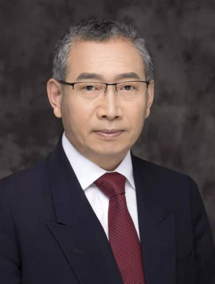
\includegraphics[width=0.6in,height=0.8in,clip,keepaspectratio]{fig/yanghz.png}}]{Huazhong Yang}
  \footnotesize
  (M’97-SM’00-F’20) received B.S.   degree in microelectronics in 1989, M.S. and Ph.D.   degree in electronic engineering in 1993 and 1998,   respectively, all from Tsinghua University, Beijing.   In 1993, he joined the Department of Electronic   Engineering, Tsinghua University, Beijing, where   he has been a Professor since 1998. Prof. Yang   was awarded the Distinguished Young Researcher by   NSFC in 2000, Cheung Kong Scholar by the Chinese   Ministry of Education (CME) in 2012, science and   technology award first prize by China Highway and   Transportation Society in 2016, and technological invention award first prize   by CME in 2019. He has been in charge of several projects, including   projects sponsored by the national science and technology major project, 863   program, NSFC, and several international research projects. Prof. Yang has   authored and co-authored over 500 technical papers, 7 books, and over 180   granted Chinese patents. 
  His current research interests include wireless sensor   networks, data converters, energy-harvesting circuits, nonvolatile processors,   and brain inspired computing. 
  He has also served as the chair of Northern   China ACM SIGDA Chapter science 2014, general co-chair of ASPDAC20,   navigating committee member of AsianHOST18, and TPC member for ASPDAC05, APCCAS06, ICCCAS07, ASQED09, and ICGCS10.  
\end{IEEEbiography}

% You can push biographies down or up by placing
% a \vfill before or after them. The appropriate
% use of \vfill depends on what kind of text is
% on the last page and whether or not the columns
% are being equalized.

%\vfill

% Can be used to pull up biographies so that the bottom of the last one
% is flush with the other column.
%\enlargethispage{-5in}



% that's all folks
\end{document}


